\documentclass[a4paper,12pt]{report}

\usepackage{packagesDonotChange/fbe_PhDtez}
\usepackage{times}
\usepackage{algorithm}
\usepackage{algorithmic}
\usepackage{epsfig}
\usepackage{amsmath, amssymb}
\usepackage{graphicx}
\usepackage[tight]{subfigure}
%\usepackage{subfigure}
\usepackage{theorem}
\usepackage{hhline}
\usepackage{booktabs}
\usepackage{fancyvrb}
\usepackage{fancyhdr}
\usepackage{epstopdf}
\usepackage{enumerate}
\usepackage{isomath}
\usepackage{upgreek}
\usepackage{url}

%\usepackage[a4paper]{geometry}
%\usepackage{setspace}
%\usepackage{parskip}
%\usepackage{upgreek}
%\usepackage{tocloft}


%\usepackage{fontspec}
\DefineVerbatimEnvironment{code}{Verbatim}{fontsize=\small}
\DefineVerbatimEnvironment{example}{Verbatim}{fontsize=\small}

\makeatletter
\newcommand{\verbatimfont}[1]{\def\verbatim@font{#1}}%
\makeatother

\providecommand{\abs}[1]{\lvert#1\rvert}
\providecommand{\norm}[1]{\lVert#1\rVert}

\setlength\fboxsep{1pt}
\setlength\subfigbottomskip{3pt}
\setlength\subfigtopskip{3pt}
\setlength{\jot}{2em}

\makeatletter
\renewcommand{\thesubfigure}{.\alph{subfigure}}
\renewcommand{\@thesubfigure}{\alph{subfigure}.\hskip\subfiglabelskip}
\renewcommand{\@@thesubfigure}{\alph{subfigure}.}

\makeatother


% this part is used to define new enviroments
% lemma 1, lemma 2
%
\newtheorem{lemma}{Lemma}
\newtheorem{theorem}{Theorem}
\newtheorem{proof}{Proof}
\newtheorem{corollary}{Corollary}
\newtheorem{definition}{Definition}


\begin{document}




%% your title will be written here be careful for the capital letters
\title{NOVEL MOBILE PRE-DIAGNOSTIC SOLUTION FOR PES PLANUS AND PES CAVUS USING IMAGE PROCESSING AND DEEP NEURAL NETWORKS}


%% write your name here

%% only first letter of name and surname is capital
%% other letters are lower case

\author{Kaan Eksen}

%% write your department here
\department{Computer Engineering}


%% write your turkish title here
\turkcebaslik{PES PLANUS VE PES CAVUS İÇİN GÖRÜNTÜ İŞLEME VE DERİN SİNİR AĞLARINI KULLANAN MOBİL ON TEŞHİS ÇÖZÜMÜ}



% write your 
\supervisor{Assist. Prof. Dr. Tacha Serif \hspace{50mm}......................................................}


\examineri{Prof. Dr. Name Surname\hspace{56mm} ......................................................}




\examinerii{Assoc. Prof. Dr. Name Surname \hspace{44mm}......................................................}

\examineriii{Assist. Prof. Dr. Name Surname \hspace{44mm}......................................................}


\dateofapproval{ .... /.... /2022}
%\dateofapproval{Day.Month.Year}



%% use for Ph.D theses  otherwise comment it
%\makephdtitle      % For Ph.D. theses


%% uncomment if it is a graduate thesis
\makemsctitle % For Proposals

\pagenumbering{roman}

\makeapprovalpage

\begin{legal}

I hereby declare that this thesis is my own work and that all information in this thesis has been obtained and presented in accordance with academic rules and ethical conduct. I have fully cited and referenced all material and results as required by these rules and conduct, and this thesis study does not contain any plagiarism. If any material used in the thesis requires copyright, the necessary permissions have been obtained. No material from this thesis has been used for the award of another degree.

I accept all kinds of legal liability that may arise in case contrary to these situations.

\begin{flushright}
Name, Last name    .......................................................
\end{flushright}
\begin{flushright}
Signature   ...................................................................
\end{flushright}

\end{legal}

\begin{acknowledgements}

I would like to express my most profound gratefulness to Yeditepe University, Computer Engineering faculty member Dr. Tacha Serif. I would also like to thank Dr. Safa Serif for his help during the tests and his suggestions on my thesis.

I would also thank my dear family, who have always stood by and supported me in every way.

I would like to thank my dear wife, Melis Eldem Eksen, who always motivates, supports me and has never-ending love.

\end{acknowledgements}


\begin{abstract}
According to previous research in this domain, about thirty percent of the world population has some kind of foot deformity. Among all the deformities, pes planus produced by a lack of the medial longitudinal arch of the foot and pes cavus produced by an excessively high plantar longitudinal arch are the foot deformities that most adversely affect the community's quality of life. Bearing in mind the above, the proposed solution aims to pre-diagnose pes planus and pes cavus through a mobile phone application using image processing and deep neural networks with the help of traditional deformity recognition methods existing in the literature. To this end, this work is composed of three studies that build upon each other, to improve the foot deformity detection precision. Accordingly, the first prototype is implemented using machine learning techniques to estimate pes planus and pes cavus using footprint approach and tested 34 participants. To benchmark this prototype, an orthopedist is asked to provide key decision-making points manually so that a comparative calculation can be performed. The comparison results of the two  showed that the expert and prototype findings were in agreement with each other more than 90 percent. As a follow up, another deformity classification method is implemented as a second study, which entailed, rearfoot angle and input from the healthcare professionals. This prototype was tested with 9 participants. Within the scope of the second study, data entries were provided by using the prototype by healthcare professionals. The system results were compared with the deformities detected by the healthcare professionals, and it was observed that the results were matched at a rate of 27.7. In the final study, the detection method developed in the first prototype is improved and tested with the test set used in the second study. The results showed that deformities detected by the physician and the system matched 83.3 percent.
\end{abstract}

\begin{ozet}
Bu alandaki önceki araştırmalara göre, dünya nüfusunun yaklaşık yüzde otuzunda bir çeşit ayak deformitesi vardır. Tüm deformiteler arasında, ayağın medial longitudinal arkının eksikliğinden kaynaklanan pes planus ve aşırı yüksek plantar longitudinal arkın oluşturduğu pes kavus, toplumun yaşam kalitesini en olumsuz etkileyen ayak deformiteleridir. Yukarıdakiler göz önünde bulundurularak önerilen çözüm, literatürde var olan geleneksel deformite tanıma yöntemleri yardımıyla görüntü işleme ve derin sinir ağları kullanılarak bir cep telefonu uygulaması aracılığıyla pes planus ve pes kavus ön teşhisini yapmayı amaçlamaktadır. Bu amaçla, bu çalışma, ayak deformitesi tespit hassasiyetini geliştirmek için birbiri üzerine inşa edilen üç çalışmadan oluşmaktadır. Buna göre, ilk prototip, pes planus ve pes kavusu tahmin etmek için makine öğrenimi teknikleri kullanılarak 34 katılımcı ile test edilmiştir. Bu prototipi kıyaslamak için bir ortopedistten, karşılaştırmalı bir hesaplamanın yapılabilmesi için kilit karar verme noktalarını manuel olarak sağlaması istenir. İkisinin karşılaştırma sonuçları, uzman ve prototip bulgularının \%90'dan fazla birbiriyle uyumlu olduğunu göstermiştir. Bunu takiben, ikinci bir çalışma olarak, arka ayak açısı ve sağlık profesyonellerinden girdi içeren başka bir deformite sınıflandırma yöntemi uygulanmaktadır. Bu prototip 9 katılımcı ile test edilmiştir. İkinci çalışma kapsamında sağlık profesyonelleri tarafından prototip kullanılarak veri girişleri sağlanmıştır. Sistem sonuçları sağlık profesyonelleri tarafından tespit edilen deformiteler ile karşılaştırılmış ve sonuçların 27,7 oranında eşleştiği gözlemlenmiştir. Üçüncü ve son çalışmada ise birinci prototipte geliştirilen algılama yöntemi geliştirilmiş ve ikinci çalışmada kullanılan test seti ile test edilmiştir. Sonuçlar, hekim ve sistem tarafından tespit edilen deformitelerin \%83,3 eşleştiğini göstermiştir.
\end{ozet}


%these are automatically generated
\tableofcontents
\listoffigures
\listoftables


\begin{symabbreviations}

\sym{API}{Application Programming Interface}
\sym{BMI}{Body Mass Index}
\sym{CDC}{Centers for Disease Control and Prevention}
\sym{GDPR}{General Data Protection Regulation}
\sym{JWT}{JSON Web Tokens}
\sym{KVKK}{Turkish Data Protection Authority}
\sym{Lidar}{Light Detection and Ranging}
\sym{MQ}{Message Queue}
\sym{OMCS}{Optical Motion Capture System}
\sym{RGB}{Red Green Blue}
\sym{RDBMS}{Relational Database Management System}
\sym{HSL}{Hue Saturation Lightness}
\sym{RFC}{Request for Comments}
\sym{SSL}{Secure Socket Layer}
\sym{UI}{User Interface}

\end{symabbreviations}

\pagenumbering{arabic}


\chapter{INTRODUCTION}\label{chp:Introduction}

Although not very aware of it, having healthy feet is of critical importance for the individual. Since the feet form the basis of the body in terms of posture, balance and support, any negativity in the foot structure affects the whole body. For example, we may have difficulty performing activities that we always do, such as climbing stairs or walking, due to a foot problem. This affects our quality of life negatively.

Recently, foot diseases have increased between 61\% and 79\% \cite{pita2017flat, menz2010characteristics}. One of these diseases is foot deformation. It is estimated that about a third of the population has some form of foot deformity. Even though pes planus and pes cavus are not the most common deformations in population, they are the foot deformations that most affect the productivity of individuals. Therefore, diagnosing and treating pes planus and pes cavus is extremely important for society. 

Pes planus is described as a decrease in the slope of the medial longitudinal arch. The prevalence of pes planus in the specific age groups varies between $<$1\% and 28\% \cite{ccilli2009prevalence, pfeiffer2006prevalence, abdel2006flat, chen2009flatfoot}. On the other hand, pes cavus is described as an increase in the plantar longitudinal arch slope. In addition, pes cavus is relatively less common than pes planus \cite{kharbuja2017prevalence}. 

In the literature, there are many methods for detecting pes planus and pes cavus, divided into two categories: non-anthropometric and anthropometric. Anthropometric methods require external tools such as a digital radiography system. Although the literature has proven that radiological imaging provides precise detection, it is not a suitable method for remote detection. Therefore, this work has been carried out with non-anthropometric methods such as arch height index and Rearfoot angle.

The first aim of this study is to remotely diagnose pes planus and pes cavus via mobile applications. However, remote diagnosis of pes planus and pes cavus is extremely difficult as there is no reference point. Therefore, deep learning networks will be used to find the reference (e.g. foot) in images. The second aim of the research is to model the sole of the foot to provide a more accurate preliminary diagnosis. For this, it will be tried to obtain results related to image processing and regression.

Within the framework of this research, answers will be sought to questions such as;

\begin{itemize}
  \item Whether deep learning algorithms are sufficient in foot detection?
  \item Is it possible to create the sole function with image processing?
  \item Is remote detection of pes planus and pes cavus possible with the required detection rate?
\end{itemize}

In chapter \ref{chp:Evaluation of Technology} of this work, the details of the overview of artificial intelligence, machine learning, and image processing are briefly explained. The next section (\ref{chp:Feet Deformities}) describes the medical treatments and detection methods of pes planus and pes cavus. Approaches to detecting pes planus and pes cavus are discussed in Chapter \ref{chp:Methodology}. Chapter \ref{chp:Foot Detection & Primary Diagnosis} provides an overview of the primary system first, followed by a discussion of testing and results. Next, chapter \ref{chp:Back Side Diagnosis} works on completely different pre-diagnosis algorithms and participants. Chapter \ref{chp:Inner Side Diagnosis Improvement}, which includes recent studies, discusses the improvement of the initial pre-diagnosis algorithm and its results. In the last section (\ref{chp:ConclusionsAndFutureWork}) potential improvements and new concepts for future work are mentioned.

\chapter{EVOLUTION OF TECHNOLOGY}\label{chp:Evaluation of Technology}

This chapter provides an overview of artificial intelligence, machine learning, and image processing. 

\section{ARTIFICIAL INTELLIGENCE}

Artificial intelligence (AI) is the ability of a computer to perform various activities similar to an intelligent entity. In order to understand whether these various activities are carried out by artificial intelligence, humans need observation. There are two different alternatives to observing intelligence. The first is introspection through the observation of thoughts, and the second is the observation of behavior, which is the result of intelligence activities.

In the 1930s, Alan Turing, a pioneer mathematician, took part in the construction of the first electronic computer. In 1950, he proposed the "Turing Test" to answer whether machines can think, which is shown in Figure \ref{fig:TuringTest}.

\begin{figure}[htbp]
\centering
\fbox{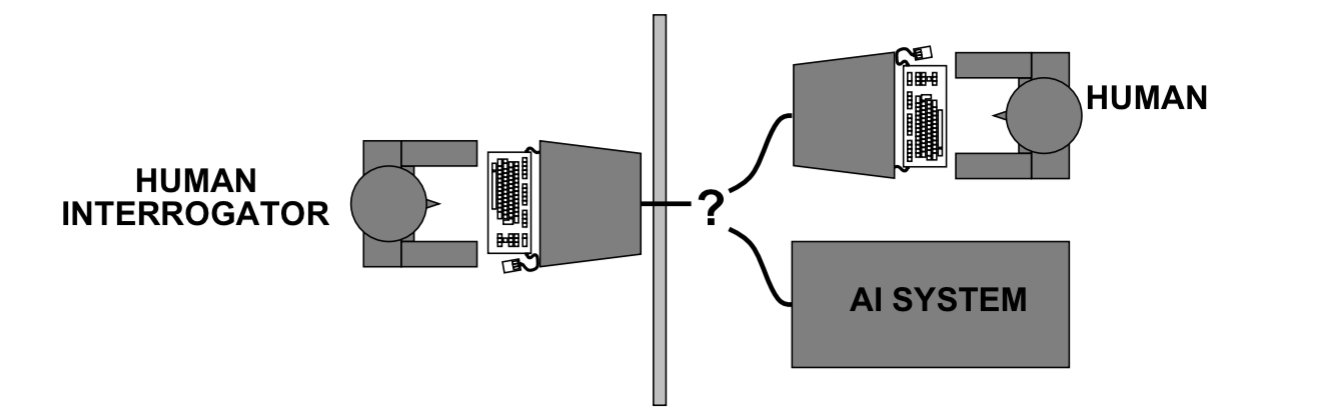
\includegraphics[width=.8\columnwidth]{figures/TuringTest.png}}
\caption{Turing test \cite{russel2010}}
\label{fig:TuringTest}
\end{figure}

In the Turing Test \cite{turing2009computing}, the subject communicates with the interrogator via a terminal. If the interrogator does not understand whether the subject is human or a machine, the subject is considered to have passed the Turing Test.

In the following years, programs such as SHRDLU \cite{winograd1972understanding}, and ELIZA \cite{mauldin1994chatterbots} were successful in the Turing Test even though they do not fully represent human intelligence. For example, the ELIZA program asks questions or forms sentences in response to the answers received from the user. Like a therapist, ELIZA asks open-ended questions. In addition, ELIZA forms the questions according to the predefined words in the answer. Hence, when there is an input sentence that contains the word "friend,'' it would reply with "Tell me about your friend.". Thus, there is no understanding or representation of human intelligence. Therefore, based on statistical information, it is possible to pass the Turing Test.

On the other hand, John Searle, who argued that machines could never have the ability to think and understand, proposed the Chinese Room Experiment \cite{preston2002views}. In the Chinese Room Experiment, a person in the locked room does not speak Chinese. An instruction manual tells what to do if specified Chinese letters have come to the room. The person who is in the room writes in Chinese using this guide. For an outside observer, there is a person who understands Chinese in the room. Understanding Chinese is not replacing symbols with certain symbols. In this respect, he suggests that computer programs will never have the ability to understand.

There are three types of AI and; they are grouped based on their abilities. Weak AI (Narrow AI) \cite{confbringsjord2003artificial} is the performing intelligent actions on a specific field (Narrow-Area) like the ability to drive a car. It is mainly emulating intelligence. General intelligence (Strong AI) \cite{confbringsjord2003artificial} is the ability to perform human-like intelligence in various tasks. It has equivalent human behavior. Lastly, Super Intelligence \cite{bostrom2003ethical} is the performing intelligent action that exceeds humans' performance in all domains.

Apart from this, there are many areas of AI such as Knowledge-based systems \cite{davis1982knowledge}, Natural Language Processing \cite{dale2000handbook}, Fuzzy Logic \cite{zadeh1996fuzzy}, Robotics \cite{brady1984artificial}. 

After a brief introduction to artificial intelligence, the following subsection will make an introduction to machine learning and machine learning types.

\section{MACHINE LEARNING}
Machine learning is the ability of machines to learn from experiences, make decisions regarding similar situations in the future, and produce solutions to problems \cite{booksmichie1994machine}. Therefore, machine learning makes generalizations for a new related event by searching previous cases and outcomes \cite{booksmichie1994machine}.

There are three types of learning methods: Supervised, Unsupervised, and Reinforcement (Figure \ref{fig:MachineLearningTypes}). The first one, Supervised Learning, requires an external intervention or an internal mechanism to achieve the desired output values. The secondary, Unsupervised Learning, utilizes  the analysis of the inputs without external intervention. Last but not least, Reinforced Learning, acquires knowledge by interacting with its surrounding environment and processing the data via a trial and failure approach \cite{sathya2013comparison}.

\begin{figure}[htbp]
\centering
\fbox{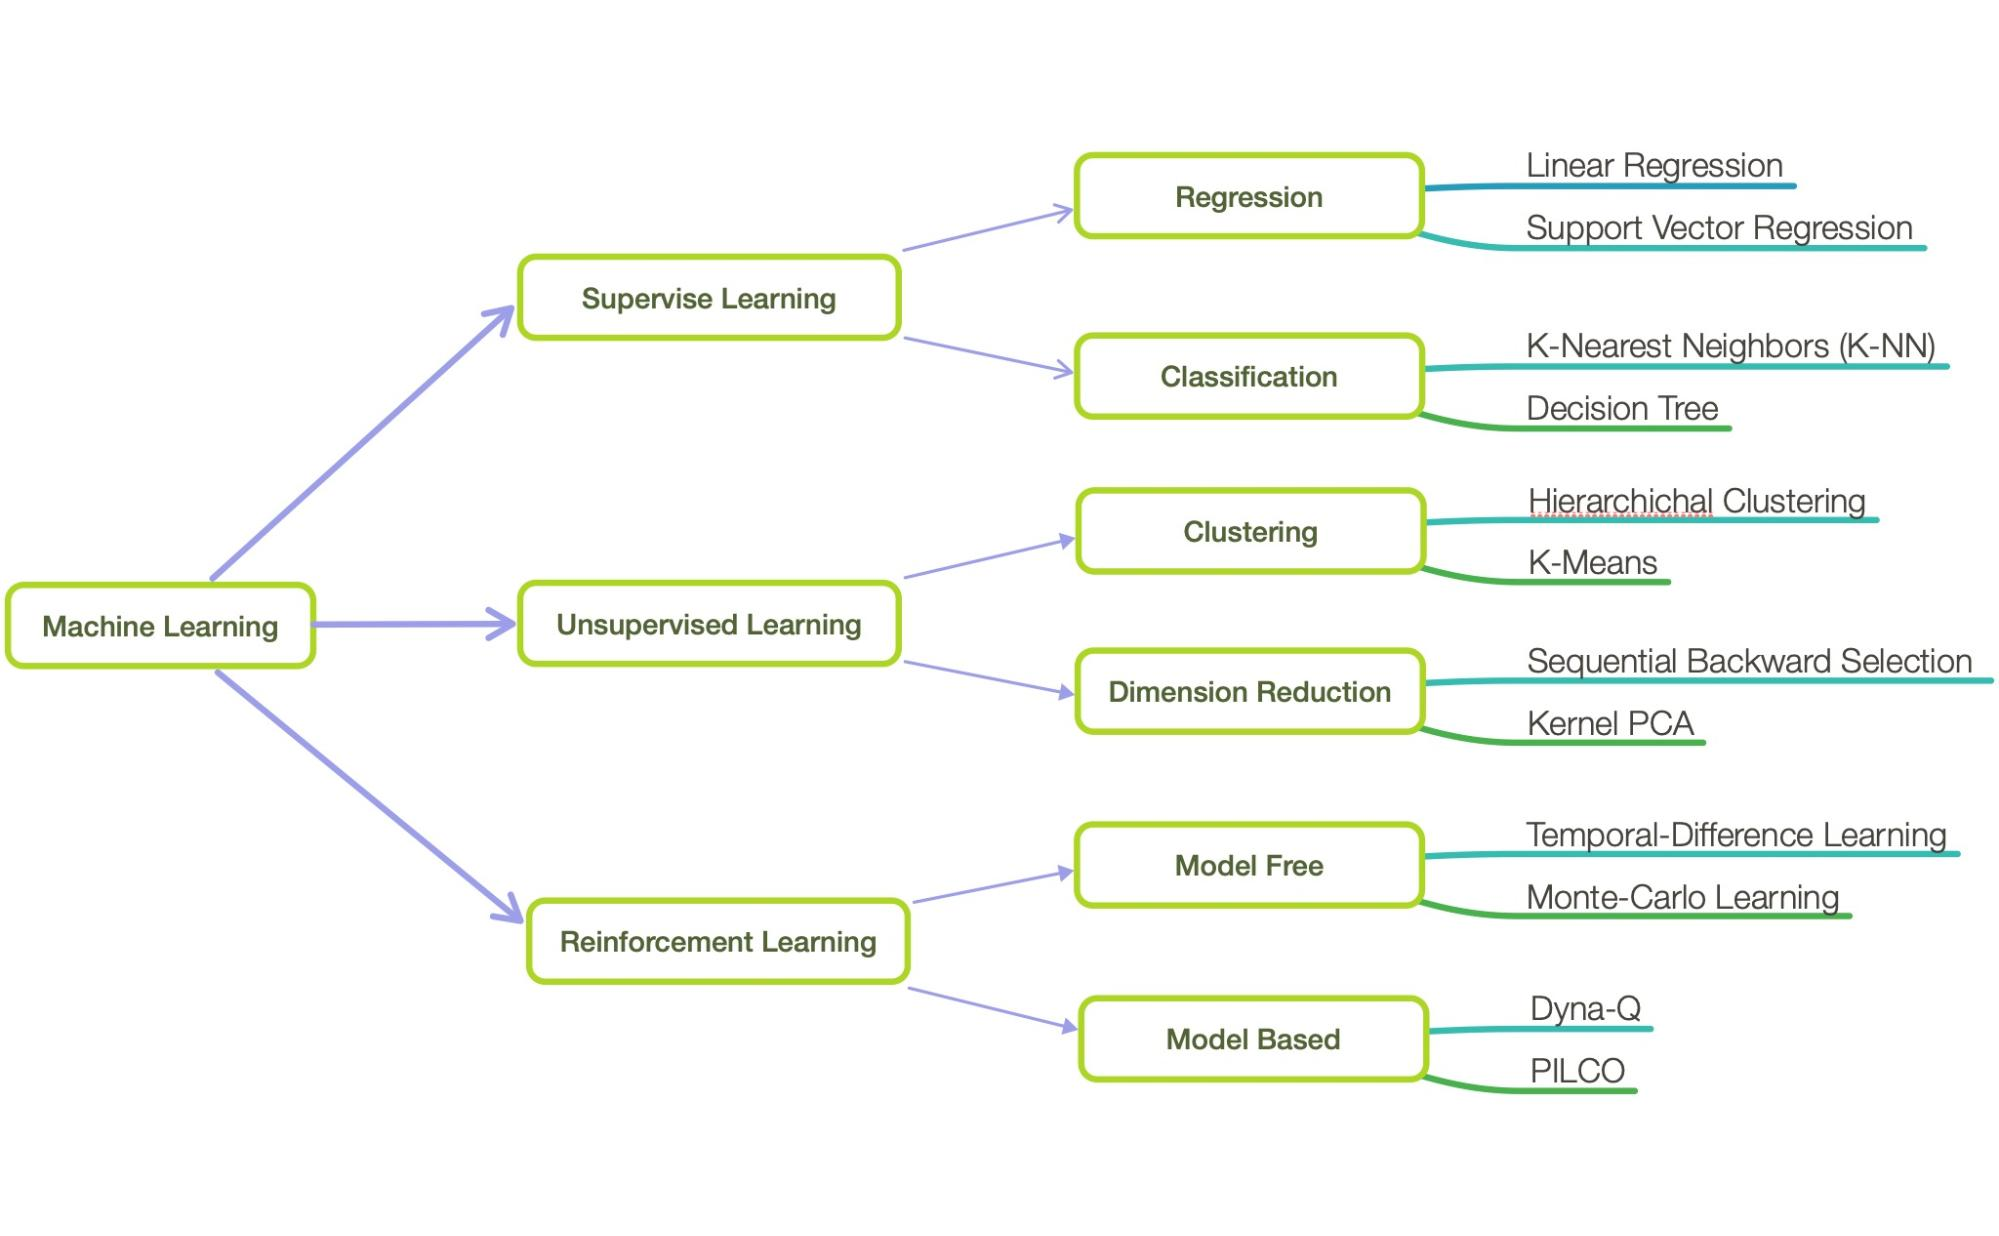
\includegraphics[width=.8\columnwidth]{figures/MachineLearningTypes.jpg}}
\caption{Machine learning types}
\label{fig:MachineLearningTypes}
\end{figure}

\subsection{Supervised Learning}

In supervised learning, both the input and output values are feeded to the algorithm in the learning phase. Therefore in the learning stage, the application processes input values and compares the desired output values with the result of the application. The difference between expected and output is treated as an error. The error value is calculated by the performance function. Result of the performance function is returned to the system to minimize this error. As a result, this process continues until the error is minimized.

In this error minimization, the algorithm generalizes outputs based on provided input data (i.e. Test Set) which is also called a supervised learning algorithm. This process could result in four main problems. We will go through each of these problems. 

The first one is the Bias-Variance trade-off \cite{geman1992neural} (Figure \ref{fig:BiasAndVariance}). A supervised learning algorithm has a high variance in predicting results with a significant deviation from the mean and other predictions when training in various practice collections. Therefore, the variance measures the contiguity of the data predicted by the model to the actual data. On the other hand, supervised learning algorithms are highly biased if inaccurate when forecasting the output for different training sets. Therefore, the bias measures how incorrect the model is. As a result, the success of the algorithm is usually associated with the amount of bias and variance \cite{james2003variance}. In most cases, the compromise between bias and variance is inevitable. In most of the algorithms, this trade-off can be modified with a parameter or automatically. 

\begin{figure}[htbp]
\centering
\fbox{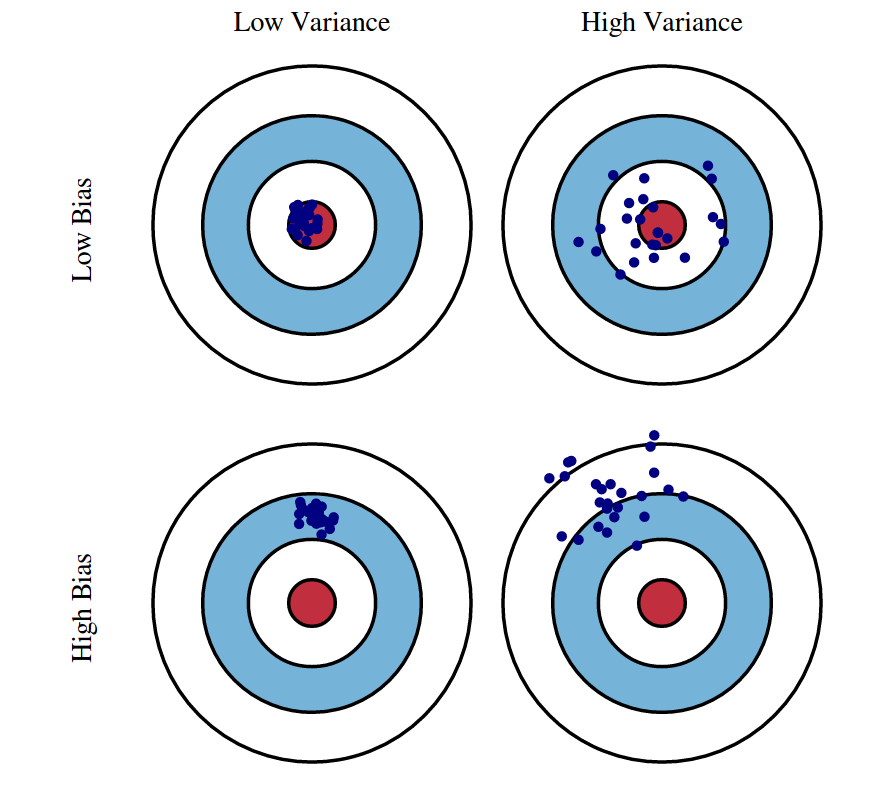
\includegraphics[width=.6\columnwidth]{figures/BiasAndVariance.png}}
\caption{Graphical illustration of bias and variance \cite{biasandvarianceillustration}}
\label{fig:BiasAndVariance}
\end{figure}

The second problem is the complexity of the problem and the amount of training data. The amount of data required to train an algorithm depends on the complexity of the problem. In relatively simple problems, the small set of training data will be enough to achieve learning. However, complex problems, which require feature extraction in multiple dimensions, need a well-distributed and an extensive training set.

The third problem is the number of dimensions in an input space. The larger the number of dimensions, the more difficult the algorithm will be to learn because of the high variance, as redundant dimensions hide features. For this problem, there are algorithms to reduce dimensions like autoencoders. Another approach for this problem would be manually extracting features before feeding them to the algorithm. Another strategy would be fine-tuning the supervised learning algorithm to low variance, and high bias may also solve the problem.

Apart from this, there is a possibility of overfitting in complex problems even if there is no noise. This type of overfitting is related to algorithms being unable to model the training data, also called deterministic noise. There are a few possible solutions to this problem. The first possible solution is removing data which caused overfitting from the data set by hand. Another approach is to use other algorithms to remove data that caused overfitting from possible errors from data sets. Another strategy would be to use early stopping to prevent overfitting. For example, the drop-out layer is used in deep neural networks to prevent overfitting.

Supervised learning is used to tackle two types of problems: Regression and Classification. Regression is a collection of statistical techniques to predict the associations between variables. It tries to model and analyze multiple variables when concentrating on the connection between a dependent variable and one or more unrelated elements. Moreover, regression is used extensively for prediction and projection.

There are two types of regression - namely, parametric and non-parametric. In parametric regression, the number of dimensions is predefined, such as Linear Regression and Ordinary Least Squares. On the other hand, non-parametric regression has no defined dimensions. As a result, regression models are often helpful in prediction, even if the assumptions are moderately wrong. Nevertheless, in many cases, regression models can not operate optimally. In the following paragraphs, we will examine a few Regression algorithms.

The linear regression method is a statistical technique that establishes a linear relationship between the independent variable and the dependent variable to estimate the feature variable \cite{tan2016introduction}. In a linear regression equation, where an example is shown in Equation \ref{linear_regression_equation}, \(x\) represents estimator for a problem, \(y\) is the response variable a the slope of the regression line is \(a_1\) and, \(b_1\) is the point at which the regression line intersects the ordinate axis.

\begin{equation} \label{linear_regression_equation}
y = a_1x + b_1x
\end{equation}

The main working principle of the support vector machine (SVM) is to divide the data into the broadest categories that separate them from each other, which is based on Vapnik–Chervonenkis theory developed by Vladimir Vapnik and Alexey Chervonenkis. SVM is successfully used in applications such as pattern recognition, time series analysis, and classification. SVM can be applied to both linear and non-linear data. The regression process is carried to the high dimensional feature spaces by the kernel function in non-linear data.

The other type in which supervised learning is used is a classification that assigns each input vector to a finite number of discrete categories \cite{harrington2012machine}. One of the most known examples of this classification is classifying emails as spam or not. Beside that, machine learning studies for classification are used in various fields such as stock estimation, customer risk analysis for bank credit, earthquake prediction, text classification, disease diagnosis, genetic studies. In the following paragraphs, few classification algorithms were examined.

K-Nearest Neighbor Algorithm (K-NN) is a memory-based classification, where its popular use is in the data mining domain. In K-NN, after the classes of the sample set are determined, the method determines which new observation belongs to which class. Here, the samples are considered a point in n-dimensional space, and the parameter k, the number of neighbors closest to the given point, is determined \cite{cover1967nearest}. The distances of all other points to the given point are calculated individually because of this method based on distance calculation. 

\begin{equation} \label{euclidean_distance_equation}
d(x,y) = \sqrt{\sum_{j=1}^{N}(x_j - y_j)^2}
\end{equation}

The Euclidean Distance shown in Equation \ref{euclidean_distance_equation} is commonly used to calculate the distance between observations. The smallest k is selected according to the distance values calculated here \cite{hall2008choice}.

\begin{figure}[htbp]
\centering
\fbox{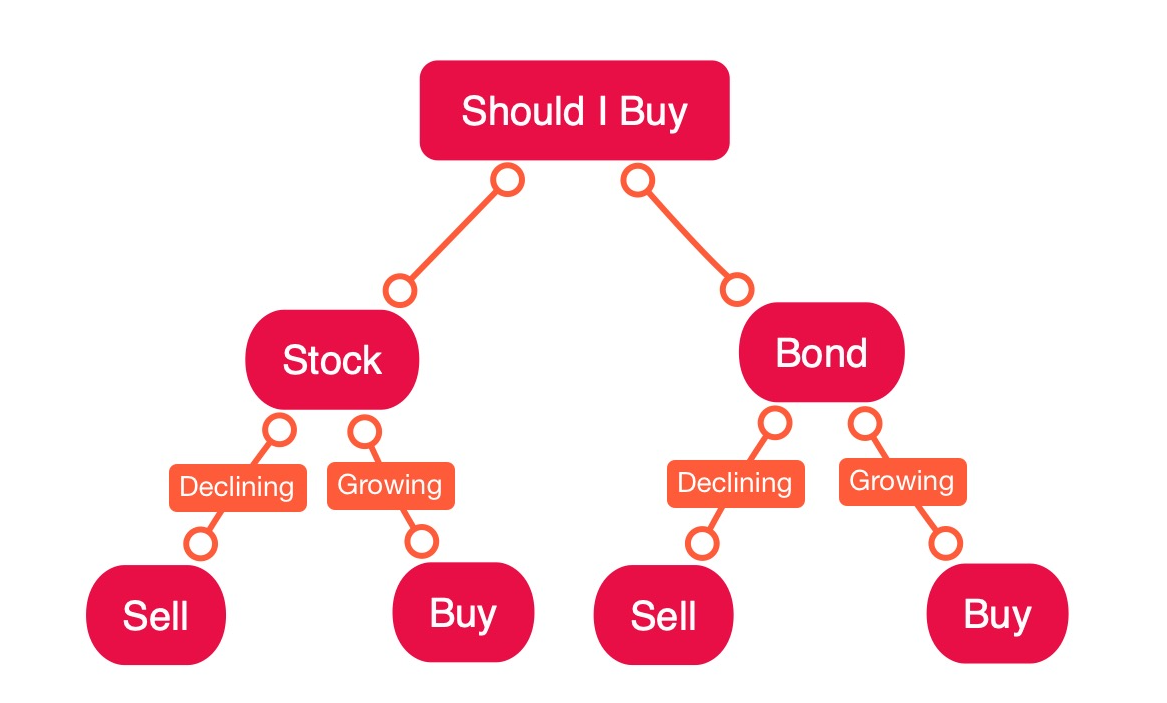
\includegraphics[width=.6\columnwidth]{figures/DecisionTree.png}}
\caption{Decision tree}
\label{fig:DecisionTreeExample}
\end{figure}

Another classification algorithm is decision trees. They consist of internal decision nodes and end leaves (Figure \ref{fig:DecisionTreeExample}). A decision tree tries to establish which class the data with a particular class will be included in, starting from the node with the highest information gain \cite{hssina2014comparative}. One of the most commonly used algorithm to create a decision tree in data mining is the ID3. The main principle of the ID3 algorithm is to classify objects by testing the values of their attributes \cite{jin2009improved}.

\subsection{Unsupervised Learning}

The purpose of unsupervised learning is to model the underlying structure or distribution of the data to extract information from raw data. Unlike Supervised Learning, there is no data to guide the learning process. It is generally used for clustering, finding relationships between attributes and size reduction. Besides, the results obtained with the unsupervised learning algorithm can be used for supervised learning \cite{chao2011machine}.

A critical point for unsupervised learning is that, while the information transmitted to learning algorithms is highly rich in underlying composition, the objectives and prizes for training are usually very narrow. Therefore, in this type of objective and prize, the algorithm should understand the information instead of applying it to a specific task. As a result, using unsupervised learning as a sub-task might improve the results even in supervised learning tasks (e.g., Deep Learning Tasks).

Unsupervised learning is used for clustering and dimension reduction. Clustering is a data grouping with similar characteristics in a data set. Therefore, there are high similarities within the same cluster, and there are low similarities between clusters. K-Means and Hierarchical Clustering are some of the commonly used clustering algorithms. These algorithms are frequently used in areas such as customer segmentation, market segmentation, and computer vision.

Clustering is a very fundamental task to discover unknown elements of unlabeled data. However, success measures depend on the users' demands, such as a minimum number of clusters. On the other hand, understanding the underlying knowledge in the cluster solely depends on the user. In the following paragraphs, we are examining K-Means and Hierarchical Clustering algorithms.

Hierarchical clustering (Hierarchical Cluster Analysis - HCA) is a cluster analysis technique designed to produce a cluster hierarchy. There are two types of HCA; namely  Agglomerative (Bottom-Up) and Divisive (Top-Down). Agglomerative type starts by turning each data into a cluster, and then the clusters that are close to each other in distance form a new cluster. Divisive is the opposite of Agglomerative. At first, all data is created in a single set, then this cluster is fragmented and reclustered. 

After the K value (the number of clusters) is determined by the user in K-Means, the algorithm selects random K points in the data set. Then, it calculates the distance between each point and random k-points to assign the data to a cluster. After assigning the points to clusters, k points are re-calculated based on the data in each cluster. Finally, the same distance calculation is performed according to the new k points. The method continues until a point is not assigned to relevant groups.

Real-life data has a large number of dimensions. This size of data brings complexity. This complexity also creates some problems; for example, there would be a significant increase in the amount of time and resources required to build a model. In addition, there is a high correlation between some attributes, leading to overfitting \cite{sonawale2015dimensionality}. Dimensionality reduction, which decreases unrelated features or merges attributes into smaller sets of dimensions \cite{biricik2012comparing}, helps us solve this problem. The following paragraphs examine the Kernel Principal Component Analysis (KPCA) and Sequential Feature Selection (SFS). 

KPCA is based on standard deviation, covariance, eigenvectors, and eigenvalues. The use of integral operator kernel functions and non-linear maps can correctly compute main parts in high-dimensional feature spaces associated with input space \cite{scholkopf1997kernel}.

SFA uses a greedy approach which is very useful for computationally complex problems. However, it might produce unoptimized solutions. SFA reduces or generates attributes at each iteration until the required dimension size k is reached.

\subsection{Reinforcement Learning}

Reinforcement learning is based on the reward system, which helps evaluate results coming from the environment by adapting itself to the actions it encounters  \cite{sutton2018reinforcement}. Therefore, there is no testing and training phase in reinforcement learning. Instead, the reward system tries to give an insight into the environment by evaluating the outputs produced by the system as good or bad.

Reinforcement learning has many applications, from robot control to simple board games. For example, a chessboard game contains simple rules, but the opponent's strategy is difficult to predict in advance because of possible moves. Therefore, the system trained with the reinforcement learning model evaluates each move of the opposing player and tries to make the best move against his opponent. Accordingly, the system anticipates possible moves and takes a position accordingly \cite{alpaydin2020introduction}.

Reinforcement learning can be performed both model-based and model-free. In model-based, algorithms try to predict the dynamics of the environment, such as alpha zero. On the other hand, model-free algorithms try to optimize the rewards without modeling the environment, such as q-learning.

The most well-known among the model-free reinforcement learning approaches is the Q-learning method. It is often applied to maze and search problems \cite{tijsma2016comparing, guo2004new, whitehead1991complexity}. Watkins, who first proposed this method in 1989, used the letter Q for the value function where, the method got this name \cite{watkins1989learning}.

There also many model-based reinforcement learning approaches such as World Models \cite{ha2018world}, I2A \cite{racaniere2017imagination}, MBMF \cite{bansal2017mbmf} PILCO \cite{deisenroth2011pilco}. PILCO is one of the most popular model-based reinforcement learning algorithms. Unlike other model-based models, it uses Gaussian Process for function approximation.

\section{IMAGE PROCESSING}

In digital image processing, analysis, and computer vision have made significant advances in theory and applications in recent years. They have been technological leaders in developments in many vital areas such as medical view multimedia systems, biology, metal science, robotics and manufacturing, intelligent sensing systems, remote sensing, graphic arts, and printers \cite{pitas2000digital}.


Digital image processing techniques consist of 3 different classes; these are low-level vision, mid-level vision, and high-level vision. Low-level vision algorithms are specifically digital image processing algorithms such as edges detection: their input and output are digital images. Mid-level vision algorithms consist of digital images as input and image properties as output such as object recognition, 3D reconstruction etc. High-level vision algorithms, on the other hand, uses the higher level of perception such as conceptual description of activity, intention and behavior \cite{pitas2000digital, gonzalez2002digital}. In the rest of this section, information about Low-Level Vision algorithms will be examined in detail.

\subsection{Digital Image Representation}

The image is the visual representation of the object by the capturing luminance emitted from the source. The mathematical model underlying image formation is based on the emitting source (e.g., visible light, X-rays, ultrasonic rays), the physics of the interaction of the emitting object, and the system is used (see Figure \ref{fig:PhongReflectionModel}). Such a system usually includes an optical lens, optical sensor, and image digitizer \cite{pitas2000digital}.

\begin{figure}[htbp]
\centering
\fbox{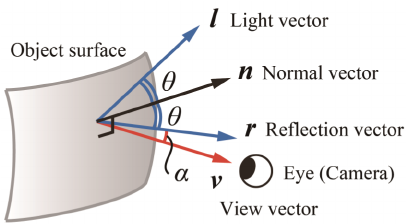
\includegraphics[width=.6\columnwidth]{figures/PhongReflectionModel.png}}
\caption{Phong reflection model \cite{kurihara2012shading}}
\label{fig:PhongReflectionModel}
\end{figure}

Digital images are generated by hardware that measures radiated energy from the source. These measurements are taken from various points across two-dimensional space to form the image. These measuring equipment are called sensors, and many different types are used. For example, sensors can interact with various parts of the electromagnetic spectrum, acoustic energy, electron emission, lasers, or other measurable signals. The electromagnetic spectrum includes visible light, infrared, ultraviolet, X-rays, microwaves, radio waves, or gamma rays (see Figure \ref{fig:EMSpectrumcolor}) [6].

\begin{figure}[htbp]
\centering
\fbox{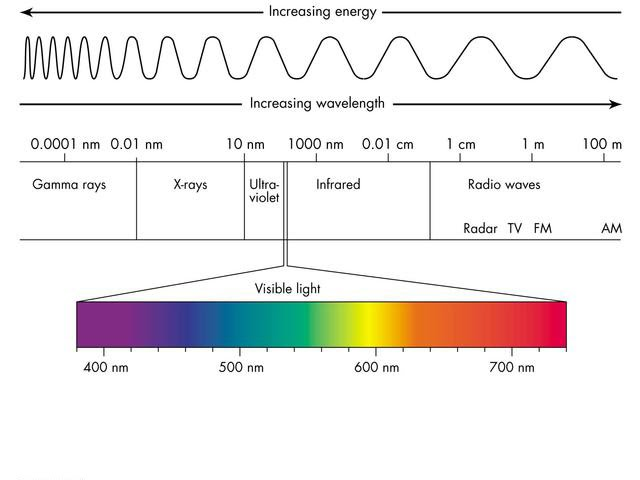
\includegraphics[width=.8\columnwidth]{figures/EMSpectrumcolor.jpg}}
\caption{Electromagnetic spectrum \cite{ElectromagneticSpectrum}}
\label{fig:EMSpectrumcolor}
\end{figure}

\subsection{Binary, Grey-Level And Color Images}

Binary images are the simplest form of imagery which can be typically represented as "black" and "white" or "0" and "1". A binary image assigns 1-bit to each pixel image which is enough to represent each pixel \cite{umbaugh2005computer, costa2000shape}. In addition, binary images are often produced according to a defined threshold value from gray-level images. Here, each pixel above the threshold value gets the value "1", and the one below the threshold value "0" \cite{umbaugh2005computer, costa2000shape}.

Gray-level images do not contain color information and only describe luminance information, also referred to as monochrome images. The number of bits used for each pixel is defined by the number of different brightness levels available. For example, a typical image contains 8-bits per pixel, which allows us to have 256 (0-255) different brightness (gray) levels \cite{umbaugh2005computer, costa2000shape}.

Color images are expressed using color models that contain three or more values for all pixels. Therefore, at least three two-dimensional matrices should express color images. Some of the most popular color display systems are RGB (Red, Green, Blue), CMY (greenish blue, magenta, yellow), and HIS (hue, vibrancy, intensity) \cite{costa2000shape}. If the 8-bit monochrome image is used as the standard model, the corresponding color image should be 24-bit, with 8 bits for all color bands (Red, green, blue) for each pixel \cite{umbaugh2005computer}.

\subsection{Image Processing And Filtering}

Image Processing can be used to remove noise from an image with a process that we can classify as image filtering. If an image has one or more noise, it should be filtered using appropriate techniques. Improved images with less noise can be obtained with special filter applications \cite{costa2000shape}

Local processing is often required for the analysis of image screens. Since the character structure of the image to be processed can vary significantly from one region to another, it is natural that local processing is necessary. Many image processes can produce output information depending on the neighbors of the pixels of the image given as input information. In reality, there are many approaches based on this idea, often using sliding windows and varying from convolution to mathematical structure \cite{costa2000shape}.

The kernel is a small matrix used in the convolutions of the image. Kernels of different sizes covering different patterns of numbers lead to different results under convolution. For example, Table \ref{tab:Kernal3_3} shows a 3x3 kernel presenting an average filter.

\begin{table}[htbp]
\begin{center}
\caption{3x3 Kernel (box blur)}
\vspace{23pt}
      \begin{tabular}{|l|l|l|}
        \hline
        1 & 1 & 1   \\
        \hline
        1 & 1 & 1   \\
        \hline
        1 & 1 & 1   \\
        \hline
      \end{tabular}
\label{tab:Kernal3_3}
\end{center}
\end{table}

Convolution is applied by shifting the kernel on the image, usually starting from the upper left corner of the image. This operation takes place in all positions where the kernel will be applied, within the borders of the whole image, by moving the kernel. This application differs on the edges of the images. Each core position corresponds to a single pixel output calculated by multiplying the kernel values with the pixel value of the image and the sum of all these numbers together \cite{russ2010image}. Mathematically expressed formula of the convolution can be seen in \ref{convolution_kernel} where  \(\xi\) is the filter kernel and \(f(x,y)\) is the image.

\begin{equation} \label{convolution_kernel}
d(x,y) = \xi * f(x,y) = \sum_{dx=-a}^{a} \sum_{dy=-b}^{b} \xi(dx,dy) f(x + dx, y + dy)
\end{equation}

Convolution can be implemented with different kernels for various purposes such as blurring or edge detection, such as the Gaussian filter and the Sobel Edge Detection Operators. A few of the popular filters will be discussed in the coming paragraphs.

The box blur which replaces each pixel value of an image with the average value, including its neighbors and itself. Therefore, this operation results in the disappearance of pixel values that are not representative of their surroundings. This type of filtering reduces the relative differences between the neighboring pixels of the image and improves contrast by reducing noise and smoothing.

The second is the Gaussian filter, a convolution operator used to remove detail and noise and blur images. Therefore, it performs similar result to the box blur, but the Gaussian operator uses a different kernel, represented as a bell \cite{getreuer2013survey} (see Equation \ref{gaussian_filter})

\begin{equation} \label{gaussian_filter}
G(x) = \frac{1} { {\sigma \sqrt {2\pi } } } 
e^{
    {
        { - {x} ^2 }
        \mathord{\left/ {\vphantom {{ - \left( {x - \mu } \right)^2 } {2\sigma ^2 }}} \right. \kern-\nulldelimiterspace} {2\sigma ^2 }
    }
}
\end{equation}

The effect of the Gaussian operator is to blur the image, as in the box blur filter. The Gaussian standard deviation determines the degree of blurring. Kernels used for a Gaussian with a more significant standard deviation will have larger dimensions. It produces the output by averaging the Gaussian center in the direction of the pixels. Therefore, it performs a smoother operation relative to the box blur filter and reveals better edges than a Gaussian similar-sized the box blur filter \cite{getreuer2013survey}.

The last one is the median filter frequently used to reduce the noise in the images. As in the box blur, the median filter evaluates the pixels in the image together with the neighboring pixels. However, instead of taking the neighboring pixel values' average, it takes the neighboring pixel values' median and replaces the pixel value \cite{russ2010image}.

\subsection{Edge Detection}

Edges are places in the image that have significant brightness changes. Therefore, edge detection is widely used to detect the object boundaries that usually occur in the image regions. In addition, creating the image with the edges of the image can significantly reduce the amount of data while retaining most of the image information \cite{russ2010image}.

Since the edges are mainly composed of high frequencies, the edges can be detected by applying a high-pass frequency filter in the Fourier region or by convolution the image with a kernel. However, edges are detected by applying convolution with a specific kernel in practice because it is cheaper and gives better results \cite{russ2010image}.

The edges can also be found by calculating the derivatives of the image since they correspond to substantial illuminance. Therefore the edges can be detected by the maximum of the first derivative and the zero of the second derivative.

Different edge detection kernels make it possible to calculate an image's first and second derivatives. For example, Prewitt Compass Edge Detection \cite{prewitt1970object}, and Gradient Edge Detection operators \cite{bovik2010handbook} are two common approaches for calculating the first derivative of an image. 

Prewitt Compass Edge Detection involves convolution of the image by adjusting the kernel sensitivity to identify a different edge. It determines the kernel edge size and definition that produces the maximum response at a pixel location. On the other hand, Gradient Edge Detection is a second and more widely used technique. Here, the image is convoluted with only two kernels for the x-direction and y-direction. The Sobel, Roberts Cross, and Prewitt operators are the most common kernels used as gradient edge detection detectors.

In Gradient Edge Detection, the pixels related to the edge need to be defined after calculating the magnitude of the first derivative. The simplest way is to set a threshold and consider all pixels with a local value above the threshold to display edges. An alternative technique to a gradient image is to identify one pixel-wide edge at the local maximum point, which is a more common technique used by the Canny edge detection method. Canny first applies Gradient edge detection to the image and then finds the edge pixels by cutting non-maximum points and tracking hysteresis \cite{moeslund2009image}.

\chapter{FOOT DEFORMITIES}\label{chp:Feet Deformities}

Correspondingly, this chapter gives an overview of significant and relevant research in pes planus and pes cavus medical treatments and detection methods.

\section{PES PLANUS AND PES CAVUS}

Abnormalities and irregularities in the normal structure of the medial longitudinal arch cause functionally unstable conditions of the foot such as pes cavus or pes planus. Pes planus is the loss of the medial longitudinal arch of the foot that results in the entire bottom of the foot approaching or touching the ground while walking or standing \cite{wozniacka2013body} (see Figure \ref{fig:BackgroundPesPlanus}). This arch acts as a flexible and adaptable foundation for the entire body \cite{kohls2009prevalence}, and its functionality is also vital to the body as it relieves the stresses of weight-bearing during the walking cycle and stores mechanical energy within the stretched elastic ligaments \cite{da1963idiopathic}. Although it may be asymptomatic, a defective medial longitudinal arch can alter the biomechanics of the lower extremities and lumbar spine, resulting in an increased risk of pain and injury \cite{gun2012pes}.

\begin{figure}[htbp]
\centering
\fbox{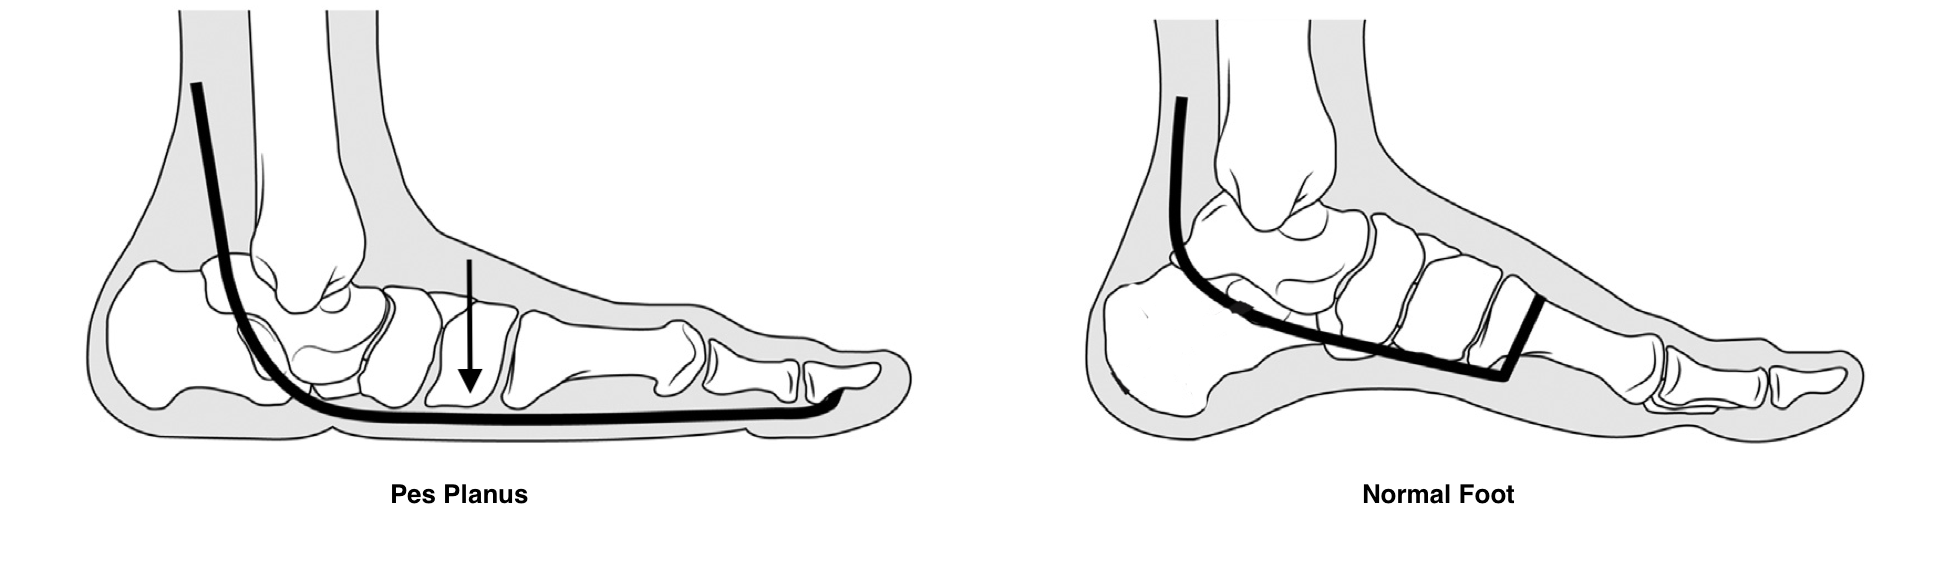
\includegraphics[width=.8\columnwidth]{KaanEksenMSc/figures/BackgroundPesPlanus.png}}
\caption{Pes Planus \cite{kim2021dynamic}}
\label{fig:BackgroundPesPlanus}
\end{figure}

Pes planus is caused by a variety of reasons that might be acquired or congenital. By the age of six, the majority of congenital pes planus abnormalities have vanished, and this is a normal aspect of human body development \cite{Mickle2006TheFO}. However, some congenital conditions can persist throughout adulthood, particularly those associated with obesity \cite{Woniacka2013BodyWA}. Pes planus can, however, develop as a result of various malformations in the extremities. One of the most prevalent causes of pes planus is functional issues with the posterior tibial tendon, which sustains the arch of the foot and allows for inversion and plantarflexion. Females over forty who have diabetes or are overweight are more likely to have posterior tibial tendon damage \cite{KohlsGatzoulis2009ThePO}. In addition, pes planus can be developed more commonly in patients with congenital ligamentous laxity secondary to Down syndrome, Ehlers Danos or Marfan. Pes planus is also common among patients who have had midfoot or hindfoot trauma, such as a navicular, first metatarsal, or calcaneal fracture, or a Lisfranc ligament complex injury.

\begin{figure}[htbp]
\centering
\fbox{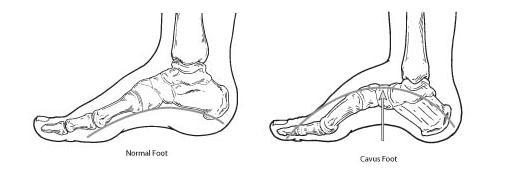
\includegraphics[width=.8\columnwidth]{KaanEksenMSc/figures/BackgroundPesCavus.jpg}}
\caption{Pes planus \cite{physiopediapescavus}}
\label{fig:BackgroundPesCavus}
\end{figure}

Pes cavus,  on the other side, is foot deformity distinguished by an elevation of the plantar longitudinal arch (see Figure \ref{fig:BackgroundPesCavus}). Clawing of the toes, posterior hindfoot deformity, plantar fascia contracture, and defects in the great toe are all common deformities associated with pes cavus. Furthermore, a common symptom of an underlying neurological disorder is pes cavus \cite{Brewerton1963IDIOPATHICPC}.

\section{MEDICAL DETECTION SOLUTIONS}

Pes planus and pes cavus have been diagnosed using ultrasonographic reviews, radiological evaluation, somatometric measurement, and clinical examination. In addition, indirect (or non-anthropometric) measurements are also utilized in the literature to detect pes planus and pes cavus, such as Inked or digital footprints (pressure measurements) and photographic \cite{gun2012pes, yalccin2010medial}. However, radiological evaluations \cite{Smith1997PrevalenceOR, Winfeld2019ManagementOP} are the most well-accepted and used approach for detecting pes planus and pes cavus in a wide range of solutions.

Chung et al. \cite{Chen2010FootprintAO} used the well-accepted radiographic detection technique to evaluate radiological data of 103 subjects' navicular and talar heights and the arch index. According to their findings, the Staheli arch index, Chippaux-Smirak index, and Clarke's angle have 85.43 percent, 90.54 percent, and 83.89 percent prediction probability in preschool-aged children correspondingly. In another research, Pauk et al. \cite{Pauk2014AssessingPP} evaluate Clarke angle and radiography data of sixty kids. Correlation between radiography and the footprints discovered in the research. Correspondingly, many research have been conducted to examine the relationship between footprint and radiography methodologies \cite{Kanatl2001FootprintAR, Yaln2010EvaluationOT, menz2005validity}.

Aside from the comparisons research presented above, several studies in the literature only use non-anthropometric methods to detect pes planus or pes cavus, such as planimeter \cite{Didia1987TheUO} or arch index \cite{Cavanagh1987TheAI, Igbigbi2002TheFR}. Aside from the comparisons research presented above, several studies in the literature only use non-anthropometric methods to detect pes planus or pes cavus, such as planimeter \cite{Didia1987TheUO} or arch index \cite{Cavanagh1987TheAI, Igbigbi2002TheFR}. Consequently, the non-anthropometric methods' applicability has been demonstrated to be viable.

On 305 Maldivians between the ages of 13 and 17, Igbigbi et al. \cite{Igbigbi2002TheFR} used an arch index (footprint ratio) to identify arc type and pes planus ratio. Subjects' foot data is obtained in this study by making an imprint of the participant's sole with ink and a piece of paper. According to the authors, the technique employed is cost-effective, resilient, and more efficient.

However, Kanatli et al. \cite{Kanatl2001FootprintAR} used 38 pre-schoolers and school-aged children with an average age of 6.4 (ages range from 3.7–11.7) to compare radiologic measures and footprint methodologies in order to determine the association between the two approaches. According to the data, there is a strong link between arch index, talo–horizontal angle, and talo-first metatarsal angle. On the other side, they discovered no link between arch index, lateral talocalcaneal angles, and calcaneal pitch.

A study that compared footprint and radiographic measures on 338 people found a decent association between the Staheli index, the Grivas Classification System, and the Chippaux-Smirak index with a similar impression \cite{gun2012correlation}. The authors emphasize, however, that there is a limited association between the radiological measurement methods calcaneal pitch angles and talo-first metatarsal angle and all three footprint measurement methods as a result of the findings. However, the authors highlight a limited association between the radiological measurement methods, the talo-first metatarsal angle and calcaneal pitch angles, and all three footprint measurement methods as a result of the findings. Furthermore, the findings show that the footprint measurement methods and talo-horizontal angle have no meaningful correlation.

\section{PES PLANUS AND PES CAVUS DETECTION TOOLS}

There are a variety of produced systems for detecting foot abnormalities, ranging from simple solutions like planimeter \cite{Didia1987TheUO} to far more advanced systems like gait analysis \cite{Buldt2015FootPI}.

Gait analysis \cite{sennotech_2021,alfoots_2021} is used by the majority of commercially available devices to detect a variety of foot abnormalities. Optical motion capture systems (OMCS) \cite{vicon_2021} are also used by some of these systems to detect foot abnormalities. Nevertheless, having this extra equipment for greater accuracy increases the required budget.

Moreover, some businesses like Sennotech's Senno Gait are designing low-cost solutions to address the market gap by reducing sensitivity. For example, Sennotech \cite{sennotech_2021} analyzes gait using low-cost sensors and AI models. As a result, these devices are less expensive and easier to use, and they provide information such as injury concerns and irregular movement.

\begin{figure}[htbp]
\centering
\fbox{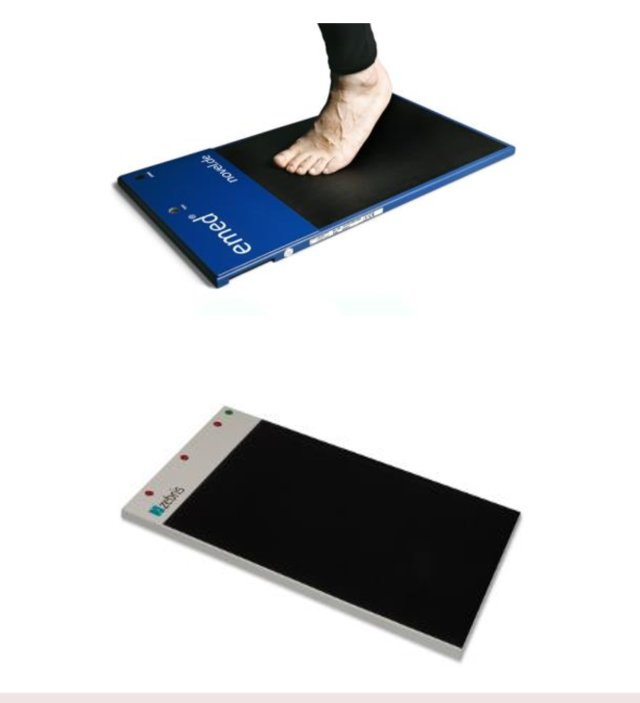
\includegraphics[width=.4\columnwidth]{KaanEksenMSc/figures/BackgroundExampleEmed.jpg}}
\caption{EMED \cite{articleFootPressure}}
\label{fig:BackgroundExampleEmed}
\end{figure}

Many research \cite{Buldt2018FootPI, articleKeukenkampDiabeticMedicine, BOSCH2010564} have employed pressure detection devices \cite{novel_2021, medilogic_2021}. These devices are far more widely available than OMCS equipment. However, they provide fewer data. Buldt et al. \cite{Buldt2018FootPI}, for example, employed EMED, a pressure sensing device, to assess pes planus and pes cavus in their research.

\chapter{METHODOLOGY}\label{chp:Methodology}

This chapter discusses and details the methodologies in the literature that are used to detect pes cavus and pes planus, and as well as deep learning.

\section{FOOT DEFORMITY DETECTION} \label{sec:MethodologyFootDeformityDetection}

One of the most efficient techniques to detect pes planus and pes cavus is using radiological scans. On the other hand, Pes planus and pes cavus may only be seen when the feet are pressed on the sole. Thereby, lateral radiographs are taken laterally or from the top of the knee and downwards for arch measures, while pushing the foot on the ground.

Many approaches for determining the state of the foot using radiological imaging have been documented in the literature. The use of calcaneal inclination angle, first metatarsal declination angle, lateral talocalcaneal angle, and Meary's angle are the most well-known of them all.

\begin{figure}[htbp]
\centering
\fbox{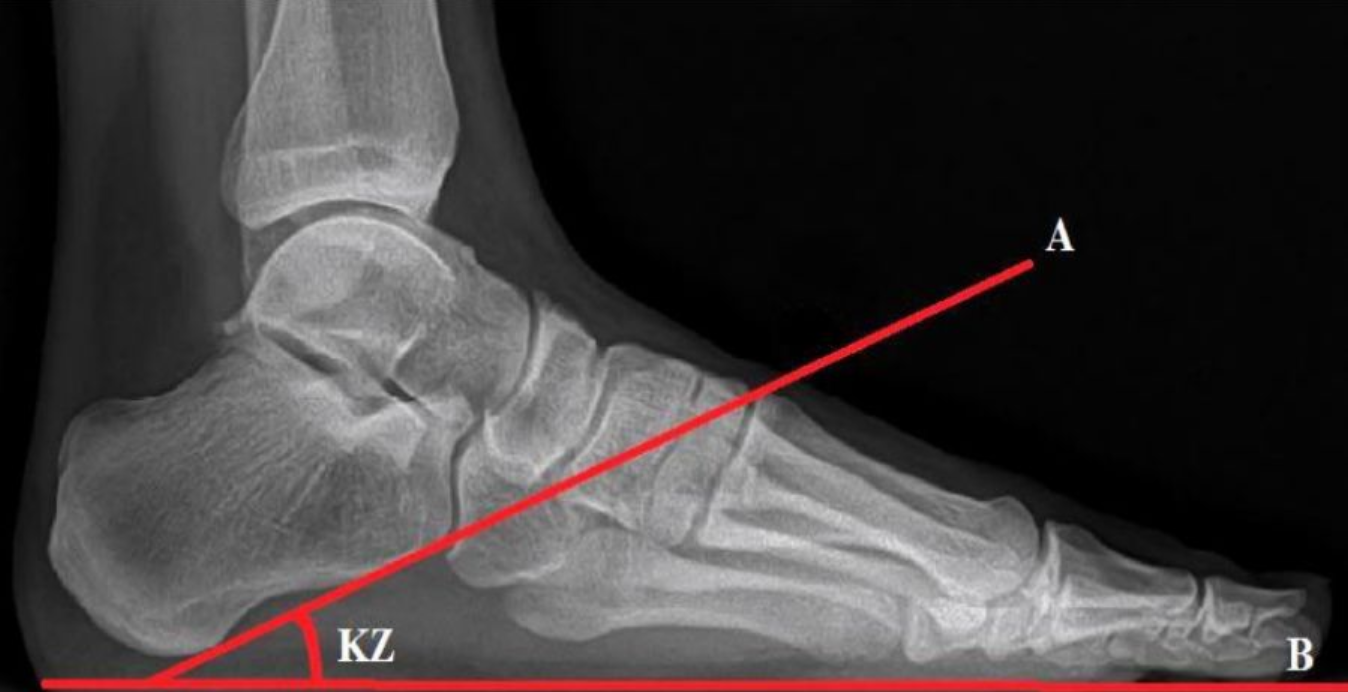
\includegraphics[width=.6\columnwidth]{KaanEksenMSc/figures/MethodologyCalcaneusInclinationAngle.png}}
\caption{Calcaneus inclination angle \cite{deniz2014ccocuklardaki}}
\label{fig:MethodologyCalcaneusInclinationAngle}
\end{figure}

The angle formed by a tangent line drawn between the lower face of the calcaneus to the ground is known as the calcaneus inclination angle (see Figure \ref{fig:MethodologyCalcaneusInclinationAngle}) \cite{deniz2014ccocuklardaki}. If the calcaneal inclination angle is between 20 and 25 degrees, the foot is considered healthy. Pes planus, on the other hand, is defined as an angle of fewer than 15 degrees \cite{flores2019adult}. However, if the angle is more than 30 degrees, it is considered pes cavus \cite{yates2009merriman}.

\begin{figure}[htbp]
\centering
\fbox{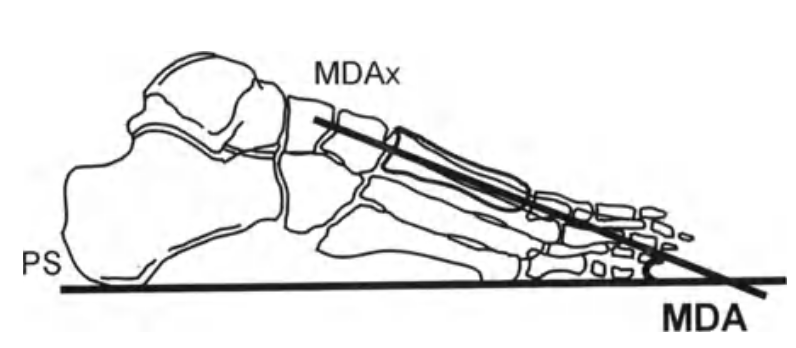
\includegraphics[width=.6\columnwidth]{KaanEksenMSc/figures/MethodologyMetatarsalDeclinationAngle.png}}
\caption{Metatarsal declination angle \cite{davies2012imaging}}
\label{fig:MethodologyMetatarsalDeclinationAngle}
\end{figure}

The metatarsal declination angle is measured by considering the horizontal surface under the sole and the calcaneal inclination axis and using a weight-bearing lateral foot radiograph (see Figure \ref{fig:MethodologyMetatarsalDeclinationAngle}). The metatarsal declination angle in the general population is predicted to be around 21 degrees [33]. In any situation, the metatarsal declination angle is greater than 30 degrees, defined as pes planus [33].

\begin{figure}[htbp]
\centering
\fbox{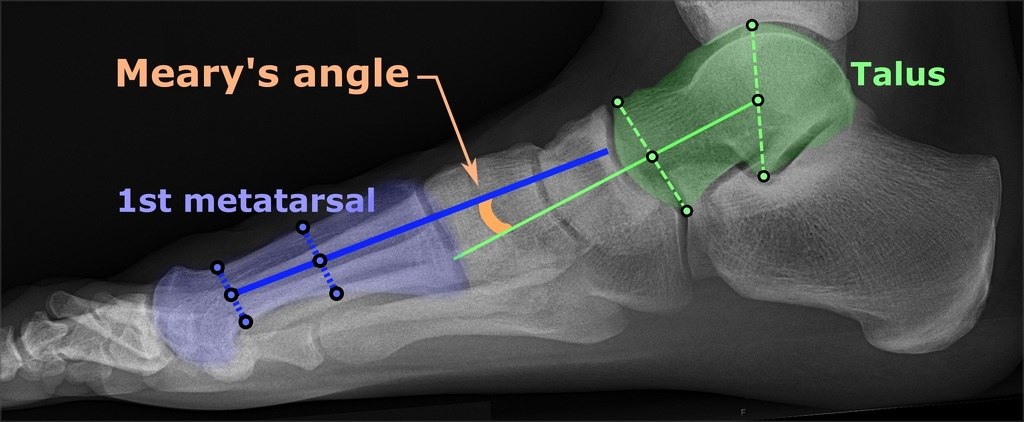
\includegraphics[width=.6\columnwidth]{KaanEksenMSc/figures/MethodologyMearysAngle.jpg}}
\caption{Meary's angle \cite{radiopaediamearysangle}}
\label{fig:MethodologyMearysAngle}
\end{figure}

Meary's angle \cite{deniz2014ccocuklardaki} is calculated by drawing a line through the centers of the longitudinal axes of the talus and first metatarsal (see Figure \ref{fig:MethodologyMearysAngle}). The foot is accepted to be pes planus if the resulting angle is more than 4 degrees (convex downward) \cite{vanderwilde1988measurements}. If the computed angle is less than -4 degrees (convex upward), the foot is classified as pes cavus \cite{banks2001mcglamry}.

\begin{figure}[htbp]
\centering
\fbox{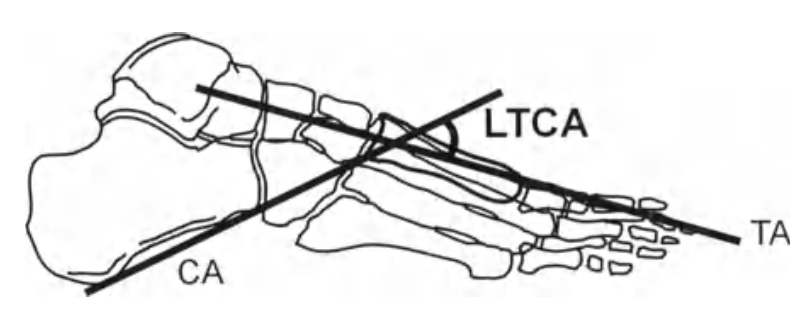
\includegraphics[width=.6\columnwidth]{KaanEksenMSc/figures/MethodologyLateralTalocalcanealAngle.png}}
\caption{Lateral talocalcaneal angle \cite{radiopaediamearysangle}}
\label{fig:MethodologyLateralTalocalcanealAngle}
\end{figure}

The calcaneal axis and the collum lateral axis form the lateral talocalcaneal angle (see Figure \ref{fig:MethodologyLateralTalocalcanealAngle}) in a weight-bearing lateral foot radiograph.  If the angle is less than 35 degrees, it is considered to be pes cavus.  In contrast, if the angle is more than 50 degrees, it is diagnosed as pes cavus.

Compared to the anthropometric pes planus and cavus detection procedures stated above, non-anthropometric measurements, while less accurate, are significantly more readily available, less expensive to do, and less harmful - i.e. do not require people to expose themselves to radiation. Therefore, Non-anthropometric procedures can be performed in large groups and in advance due to their ease of access.

The footprint approach, which involves sinking the foot into ink and then pressing it onto graph paper, is one of the most common non-anthropometric methods used in the literature. Many indexes, such as the Staheli arch and the Chippaux-Smirak indices, use graph paper to identify pes planus and pes cavus.

\begin{figure}[htbp]
\centering
\fbox{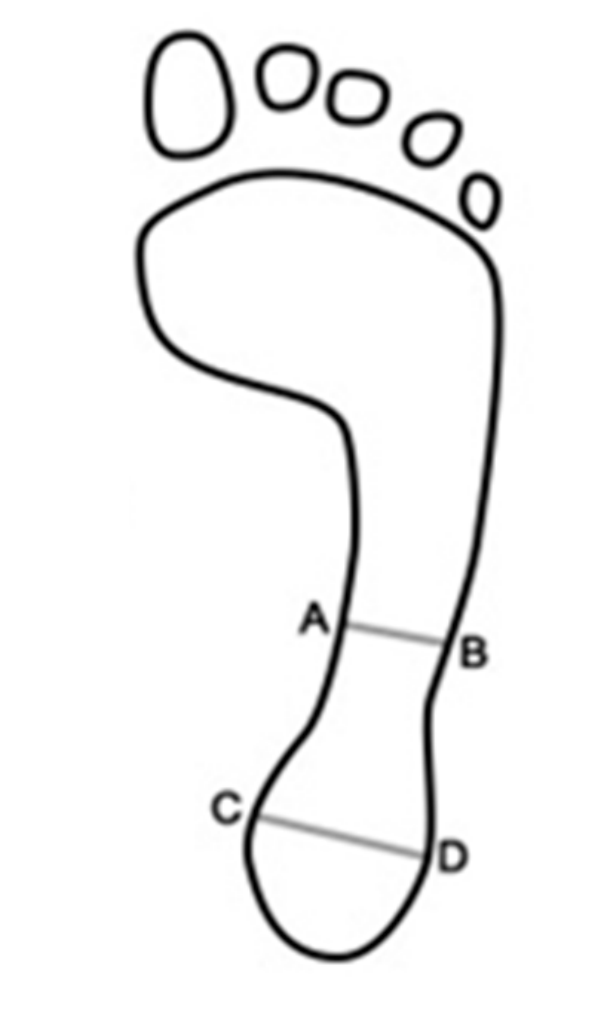
\includegraphics[width=.2\columnwidth]{KaanEksenMSc/figures/MethodologyStaheliIndex.png}}
\caption{Staheli index AB/CD \cite{radiopaediamearysangle}}
\label{fig:MethodologyStaheliIndex}
\end{figure}

By dividing the width of a foot's center part by the width of the heel region, the Staheli index is determined (see Figure \ref{fig:MethodologyStaheliIndex}). The foot is considered to be pes planus if the determined ratio (index) is more than 0.8. However, if the estimated ratio is less than 0.4, it is classified as pes cavus \cite{almaawi2019flatfoot}.

\begin{figure}[htbp]
\centering
\fbox{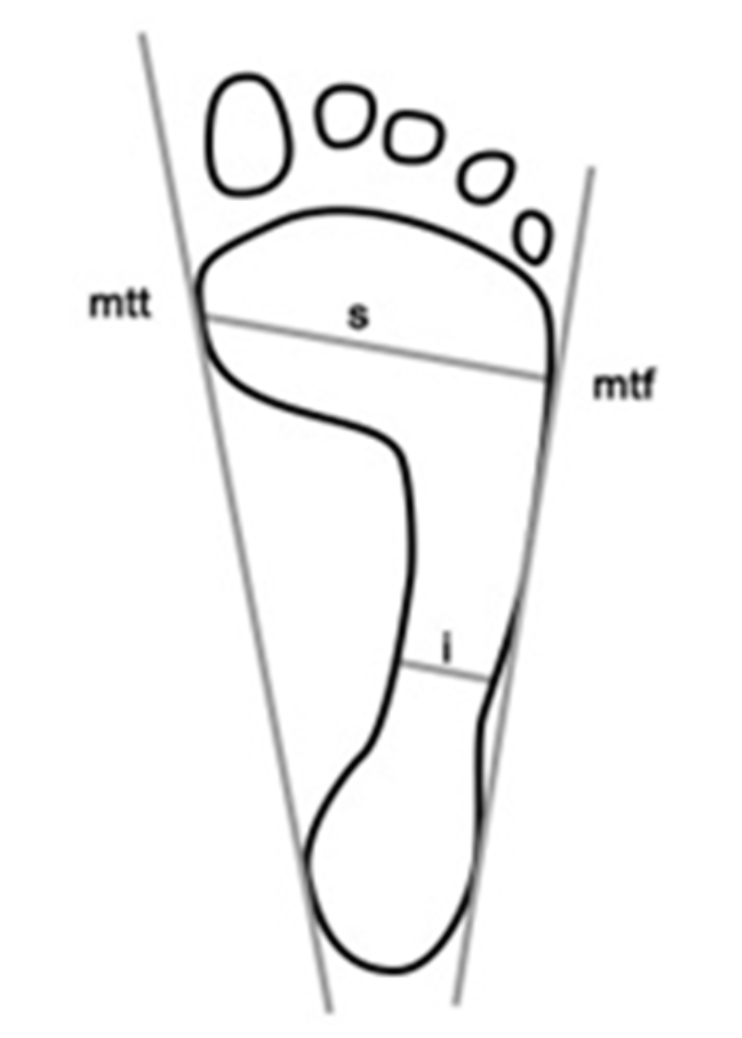
\includegraphics[width=.25\columnwidth]{KaanEksenMSc/figures/MethodologyChippauxSmirakaIndex.png}}
\caption{Chippaux-Smiraka index i/s \cite{radiopaediamearysangle}}
\label{fig:MethodologyChippauxSmirakaIndex}
\end{figure}

On the other hand, the Chippaux-Smirak Index (see Figure \ref{fig:MethodologyChippauxSmirakaIndex}) is calculated by taking into account the ratio of the midfoot's narrowest and widest regions. If the  resulting proportion greater than 0.45 in the Chippaux-Smirak Index is defined as Pes planus. On the other hand, it is considered pes cavus\cite{almaawi2019flatfoot} if the proportion is less than 0.25.

\begin{figure}[htbp]
\centering
\fbox{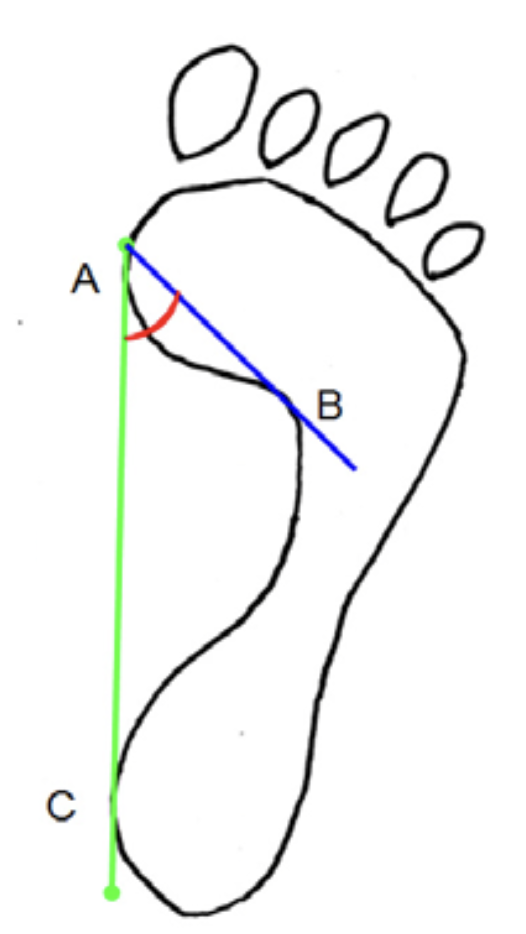
\includegraphics[width=.25\columnwidth]{KaanEksenMSc/figures/MethodologyClarkesAngle.png}}
\caption{Clarke's angle \cite{ozer2012evaluation}}
\label{fig:MethodologyClarkesAngle}
\end{figure}

The Clarke angle is formed by a line joining the tangent at the medial edge (A-C line in Figure \ref{fig:MethodologyClarkesAngle}) of the footprint and the longest vertical distance from the medial border of the foot to the point where the medial tangent intersects the edge of the forefoot(A-B line in Figure \ref{fig:MethodologyClarkesAngle}). Based on the size of the A and B lines’ angle a foot is classified as, Normal (42°–54°), mild flatfoot (35°–41°), moderate flatfoot (30°–34.9°), severe flatfoot (30°), and high arched foot ($>$ 54°) using the Clarke's angle approach \cite{hegazy2021comparing}.

\begin{figure}[htbp]
\centering
\fbox{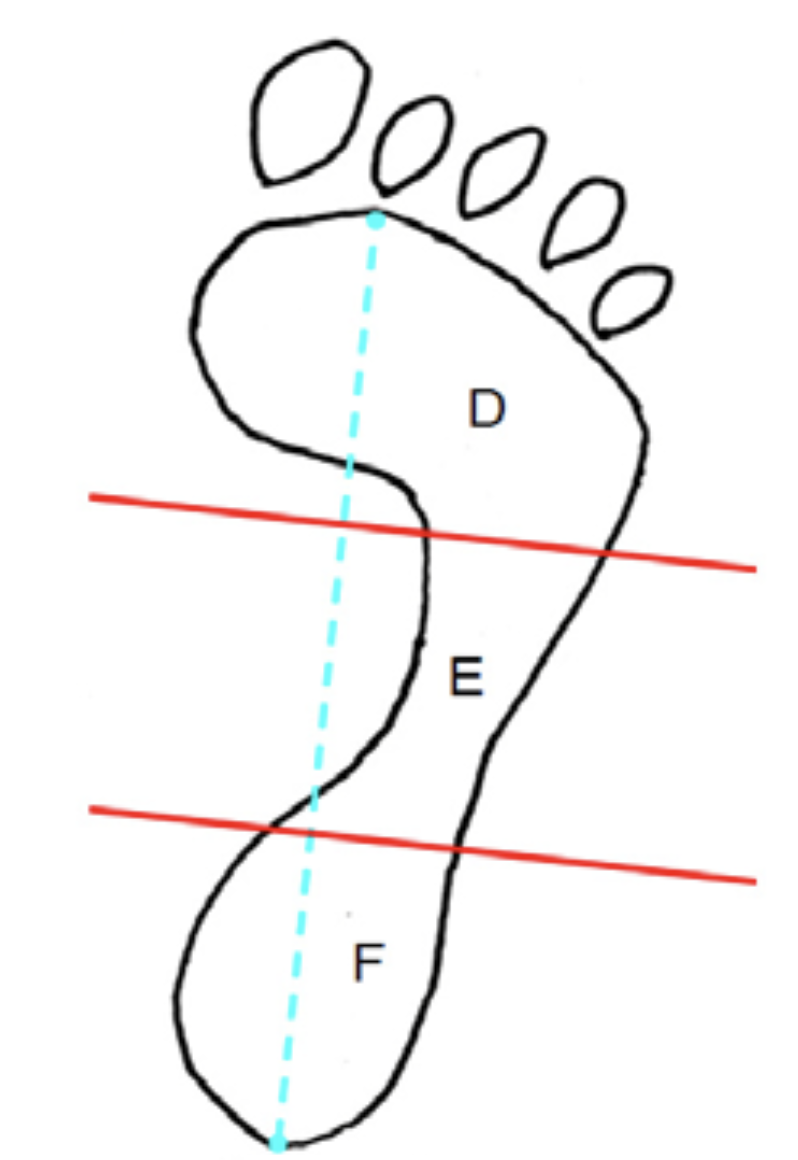
\includegraphics[width=.25\columnwidth]{KaanEksenMSc/figures/MethodologyArchIndex.png}}
\caption{Arch index E/D+E+F \cite{ozer2012evaluation}}
\label{fig:MethodologyArchIndex}
\end{figure}

The arch index is calculated by the midfoot area (E in Figure \ref{fig:MethodologyArchIndex}) in ratio to the sum of the hindfoot (F in Figure \ref{fig:MethodologyArchIndex}), midfoot, and forefoot (D in Figure \ref{fig:MethodologyArchIndex}) areas. If the ratio of the arch index is equal to or larger than 0.26, the foot is considered to be flat. If it is less than 0.21, it is considered pes cavus. Otherwise, it is a normal arch \cite{igbigbi2005arch}. 

\begin{figure}[htbp]
\centering
\fbox{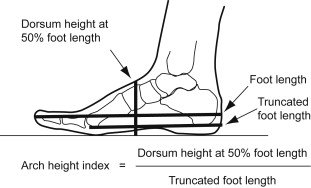
\includegraphics[width=.50\columnwidth]{KaanEksenMSc/figures/MethodologyArchHeightIndex.png}}
\caption{Arch height index E/D+E+F \cite{miller2014effect}}
\label{fig:MethodologyArchHeightIndex}
\end{figure}

There are other non-anthropometric procedures that do not require a footprint, such as arch height and rearfoot angle. Instead, these use intermediate results such as pictures to make measurements.

The arch height at 50\% of the entire foot length is divided by the truncated foot length to calculate the arch height index (see Figure \ref{fig:MethodologyArchHeightIndex}). In the arch height index average pes planus foot’s ratio is expected to be 0.35 ± 0.03 and average pes cavus foot’s ratio is expected to be 0.40 ± 0.03 \cite{hillstrom2013foot}.

\begin{figure}[htbp]
\centering
\fbox{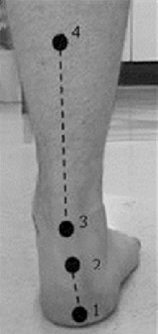
\includegraphics[width=.40\columnwidth]{KaanEksenMSc/figures/MethodologyRearfootAngle.jpg}}
\caption{Rearfoot angle critical points \cite{langley2016clinical}}
\label{fig:MethodologyRearfootAngle}
\end{figure}

Rearfoot angle is calculated using the angle between two lines, As illustrated in the figure \ref{fig:MethodologyRearfootAngle}. The lines contracted by the four points are the Achilles tendon center at the height of medial malleoli, the center of the shank posterior, 15 cm above the Achilles tendon center, and the base of the calcaneus \cite{huerta2008relationship}. If the calculated angle is between -4 and 4 degrees, the foot is classified as normal. On the other hand, If the computed angle is larger than 5 degrees and valgus, it is considered pes planus. If it is then 5 degrees and varus, it is classified as pes cavus \cite{jonson1997intraexaminer}.

\section{DEEP LEARNING}

Deep learning is a prominent object identification approach, a subset of machine learning that can be supervised (such as classification) or unsupervised. As a result, deep learning employs a large number of non-linear processing unit layers for feature extraction and conversion. Hence, each subsequent layer uses the output of the preceding layer as input and produces a classification \cite{goodfellow2016deep}.

One of the most influential aspects of deep learning is feature extraction. Low and high level (i.e. features extracted from low-level features)
can be automatically extracted from data in deep learning. Therefore, manual feature extraction has become obsolete in deep learning. However, deep learning algorithms require comprehensive data and high-performance hardware to process this data compared to other machine learning algorithms \cite{lecun2015deep}.

Deep learning is a very effective method that provides the ability to train and learn systems with large and complex probabilistic models. In order to achieve this, it uses different layers in a data representation. Therefore this provides the ability to pre-trained those layers separately. As a result, recent research shows that it provides more successful results than traditional approaches \cite{chen2015net2net, huang2013cross}.

The data's size and complexity are significant factors in deep learning training. Therefore, increased complexity and size affect the training time. Transfer learning can be used to reduce training time by using deep learning algorithms trained in similar fields \cite{goodfellow2016deep}. 

There are many deep learning architectures. Some of the significant architectures will be discussed in the following paragraphs starting with artificial neural networks then, recurrent neural networks, convolutional neural networks. 

Artificial neural networks are a building block of deep learning that perform functions such as remembering, learning, generalizing, and producing new information by mimicking the human brain. Artificial neural networks are used in many fields and applications such as fingerprint recognition \cite{baldi1993neural}, autonomous vehicles \cite{tian2018deeptest}, voice recognition \cite{melin2006voice}, meteorological interpretation \cite{hsieh1998applying}, handwriting recognition\cite{oh2002class}.

\begin{figure}[htbp]
\centering
\fbox{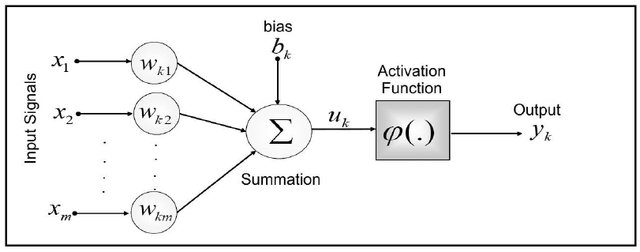
\includegraphics[width=.60\columnwidth]{KaanEksenMSc/figures/MethodologyArtificialNeural.jpg}}
\caption{Artificial neural \cite{veronez2011regional}}
\label{fig:MethodologyArtificialNeural}
\end{figure}

Artificial neurons have a straightforward structure. They consist of input, weights, bias, activation function, and output (see Figure 6). Inputs are the data coming into neurons from another artificial neuron or the initial input. The input is multiplied by a weight value and summed with the bias, which is optional. After calculating the summation, the output is produced with the help of the activation function. In addtion, each input effect can be adjusted with bias.

\begin{figure}[htbp]
\centering
\fbox{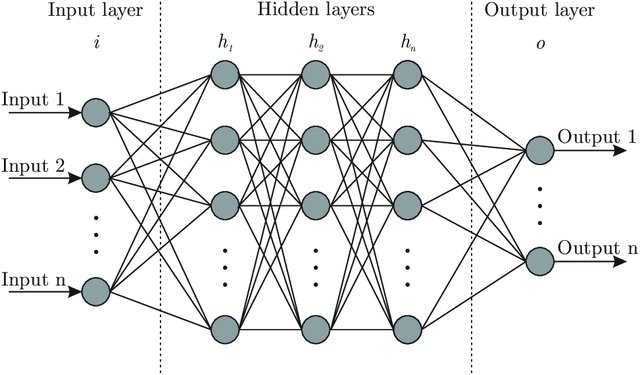
\includegraphics[width=.60\columnwidth]{KaanEksenMSc/figures/MethodologyArtificialNeuralNetwork.jpg}}
\caption{Artificial neural network\cite{bre2018prediction}}
\label{fig:MethodologyArtificialNeuralNetwork}
\end{figure}

The combination of artificial neuron cells form an artificial Neural Network. An Artificial Neural Network is made of three main layers. These are the input layer, hidden layer, and output layer (see Figure \ref{fig:MethodologyArtificialNeuralNetwork}). The input layer brings the initial data into the system, which does not undertake any processing and relays that data directly to the lower layers. Next, the data is transferred into the hidden layer for further processing. Depending on the structure of artificial neural networks, the number of hidden layers may vary. Finally, after the processing, the output layer receives that processed data and offers the final results. 

The calculated output and expected output values are processed according to the error function. Therefore, the error value is the difference between the calculated output and expected values. Finally, the calculated error value is updated using the optimization function. Various parameters, such as the number of data, the number of layers in the neural network, the activation function, and the learning rate \cite{goodfellow2016deep}, directly affect the success of artificial neural networks.

Recurrent neural networks (RNN) are another essential architecture with an internal memory structure. Their internal structure provides input history so that it correctly predicts the future. Whereas in conventional neural networks, all input data are assumed to be independent of each other, the basic idea of recurrent neural networks is to use sequential information \cite{medsker1999recurrent}. Although RNNs are considered to be able to use information in very long sequences, in theory, it is known that returning to information is very limited in practice \cite{medsker1999recurrent}.

\begin{figure}[htbp]
\centering
\fbox{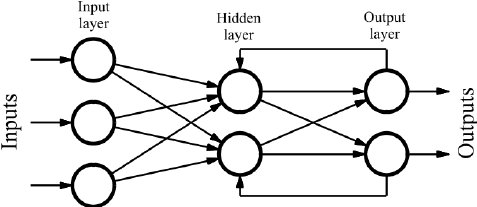
\includegraphics[width=.60\columnwidth]{KaanEksenMSc/figures/MethodologyRecurrentNeuralNetwork.jpg}}
\caption{Recurrent neural network \cite{quiza2009computational}}
\label{fig:MethodologyRecurrentNeuralNetwork}
\end{figure}

RNNs create a loop and use past data, which can be seen in Figure \ref{fig:MethodologyRecurrentNeuralNetwork}. RNNs are used in language modeling \cite{mikolov2011extensions}, machine translation \cite{cho2014learning}, speech recognition\cite{miao2015eesen}, image description creation \cite{mao2014deep}, and video tagging \cite{garg2021video}. 

\begin{figure}[htbp]
\centering
\fbox{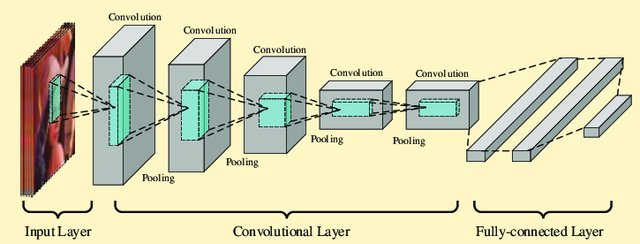
\includegraphics[width=.60\columnwidth]{KaanEksenMSc/figures/MethodologyConvolutionalNeuralNetworkExample.jpg}}
\caption{Convolutional neural network example \cite{ferracuti2019business}}
\label{fig:MethodologyConvolutionalNeuralNetworkExample}
\end{figure}

Convolutional neural networks, which are created by taking as a model the human vision system, have achieved significant success in computer vision \cite{gu2018recent, bouvrie2006notes, lavin2016fast}. They are used in many areas such as object recognition, object classification, object tracking, sentence modeling. CNN may contain many layers: the input layer, convolution layer, ReLu, pooling layer, fully connected layer, dropout layer, classification layer, and output layer (see Figure \ref{fig:MethodologyConvolutionalNeuralNetworkExample}).

The convolution layer, also known as the transform layer, is based on circulating a filter over all the input data. Filter sizes can be in different sizes such as 2x2, 3x3. The filters take the output data from the previous layer, apply the convolution operation and generate a feature map. Feature maps are regions where features specific to each filter are discovered. Edge information can also be found in this feature map \cite{goodfellow2016deep}

The convolution layer, also known as the transform layer, circulates a filter over all the input data. Filters can be in different sizes, such as 2x2, 2x3. These filters take the output data from the previous layer, apply the convolution operation and generate a feature map. Feature maps are regions where features specific to each filter are discovered. For example, edge information can also be found in this feature map \cite{goodfellow2016deep}.

The primary purpose of the pooling layer is to reduce the size of the input data. As the data leaves this layer, size reduction and information loss occur. This loss benefits the neural network as it reduces the computational load and prevents the system from memorizing \cite{goodfellow2016deep}. Another layer that causes information loss is the dropout layer. Using this layer, some of the data is not transmitted to the next layer


The fully connected layer is linked to all areas of the previous layers used in many network designs. Also, multidimensional data is converted to one dimension in the classification layer using the flattening method. As a result, classification is performed on one-dimensional data \cite{goodfellow2016deep}.

There are many object detection applications that have been created for the purposes such as people counting \cite{nogueira2019retailnet}, autonomous vehicles \cite{rausch2017learning}, and face detection \cite{yang2015facial}. The general principle of object detection is to recognize a previously defined object class in a new image and define the positions of each object it detects in this image using a rectangle that encloses the entire object \cite{goodfellow2016deep}.

Many accurate and fast algorithms are available for object detection and tracking. However, the most straightforward deep learning approach for object detection and object tracking in deep learning is convolution neural networks.  One of the disadvantages of this approach is that it does not recognize objects of different sizes. This requires each of them to be processed separately and requires a lot of computation time. Nevertheless, many neural networks are available for object detection, such as Fast R-CNN \cite{girshick2015fast}, Faster R-CNN \cite{ren2016faster}, YOLO\cite{redmon2018yolov3}.

Semantic segmentation, one of the challenging problems in image classification, is defined as the labeling of raw pixels in an image with an object category. Deep learning approaches such as FCN and DeepLabV3 have been developed for semantic segmentation. For instance, an image is acquired using the Fully Convolutional Network (FCN) approach. Then, a segmented image of the same size as the input is produced. In this way, different probability values can be obtained for each pixel in the input image \cite{long2015fully}. DeepLabv3 is an approach built on top of the ResNet-101 \cite{deepResidualLearning2016} architecture by adding Atous Spatial Pyramid Pooling (ASPP). ASPP applies convolution filters with different void ratios on the ResNet output to obtain feature maps with different details according to the void ratios of the filters \cite{chen2017rethinking}.
\chapter{STUDY I - FOOT DETECTION AND PRIMARY DIAGNOSIS}\label{chp:Foot Detection & Primary Diagnosis}

This chapter provides an overview of the primary system. Unlike other example solutions, the proposed approach will contain progressive updates with collected data over time. That is why the initial study contains fundamental structures to conduct the research. Accordingly, in Section \ref{sec:StudyIAnalysisAndDesign}, discusses general system analysis and design decisions. Section \ref{sec:StudyIImplementation} covers detailed implementation of the prototype system, and lastly, Section \ref{sec:StudyITestAndEvaluation} presents evaluation phase and initial test results.

\section{ANALYSIS AND DESIGN}\label{sec:StudyIAnalysisAndDesign}

The system, when used by patients, calculates a preliminary detection of potential pes planus and pes cavus. Therefore, end-user interface, healthcare interface, back-end services, and database are needed. Each structure contains its own development life-cycle to provide the best results. The proposed structure of the system can be seen in Figure \ref{fig:GeneralArchitectureDiagram}.

\begin{figure}[htbp]
\centering
\fbox{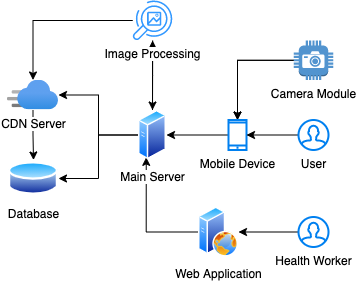
\includegraphics[width=.6\columnwidth]{figures/GeneralArchitectureDiagram.png}}
\caption{Architecture diagram}
\label{fig:GeneralArchitectureDiagram}
\end{figure}

The goal of the study is to assist the medical staff in detecting pes planus and pes cavus and reduce the workload of medical staff. The system to be formed at the end of the study should provide basic functional requirements and as well as non-functional requirements, which are detailed below;
\begin{itemize}
  \item Detection of pes planus and pes cavus with at most accuracy in provided images.
  \item Detects predefined extreme health cases and redirects users to healthcare professionals.
  \item Verify the results manually with an interface for experts
  \item View detection results
  \item Provide statistical reports about pes planus and pes cavus
  \item Provide the functionality to a wide range of users on multiple mobile platforms.
  \item Store all confidential information securely
  \item Store all essential information in non-volatile storage
  \item Design scalable system for large scale usage
\end{itemize}

\begin{figure}[htbp]
\centering
\fbox{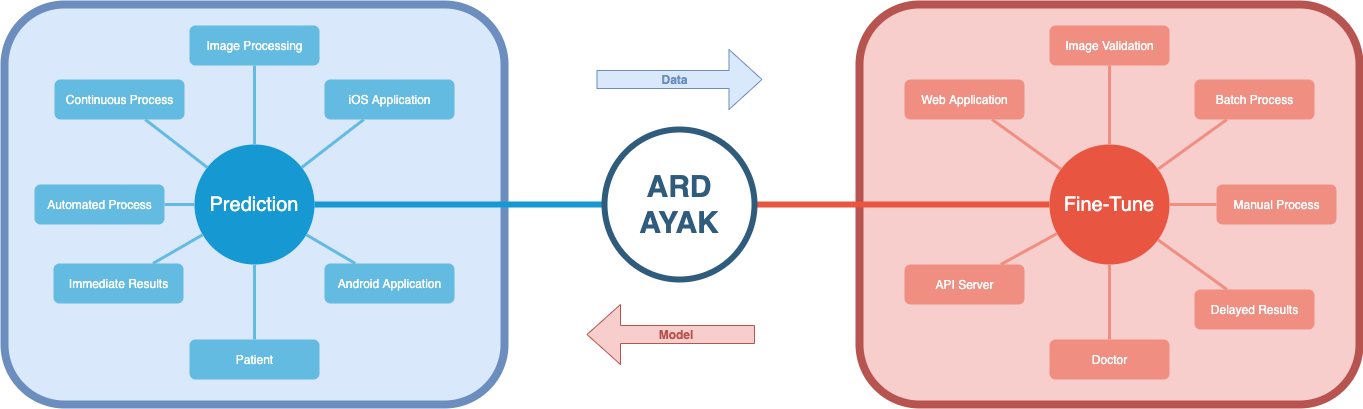
\includegraphics[width=.9\columnwidth]{figures/PredictionAndFinetuneModules.png}}
\caption{Prediction and fine-tune modules}
\label{fig:PredictionAndFinetuneModules}
\end{figure}

Furthermore, all the services should not be accessible by unauthorized users since the system contains confidential information. Therefore, the same authorization process should be used in all information access. In addition, for research purposes, user data will be purified from user-identifying information when calculating measurement methods imposed by KVKK and GDPR, such as phone numbers.

The system should contain two essential components in order to provide a stable service: the prediction and fine-tune modules. In addition, modules should support each other and improve the process, as shown in Figure \ref{fig:PredictionAndFinetuneModules}.

\subsection{ Prediction Module }

The prediction module should essentially consist of two parts, namely end-user and pre-diagnosis application. The end-user application will provide remote access, which is one of the priorities of the system, to the user. Thus, patients will be provided with healthcare services without going to the hospital. To this end, mobile applications should provide services to 95 percent of the mobile operating systems in the market, which are mainly made of iOS and Android operating systems. After user information is collected through the end-user application, pre-diagnosis application will be used to diagnose the user and provide results.

In the prediction module, user information collection is one of the fundamental parts. Information collection should be divided into three fundamental headings: essential, health, and foot information. 

The essential information collection part focuses on differentiating end-users. Therefore, unique properties such as users' phone numbers or email addresses should be collected as part of this heading. Furthermore, gender, birth date, weight, and height should also be collected to analyze the population variance. Even if it is not related, the terms and conditions document that asks the user to confirm data usage and storage permission also should be viewed and agreed upon under this heading.

The second part is the health information collection which focus on detecting health issues related to pes planus and pes cavus. However, this part also requires the system to detect the evaluation requirement of health professionals for critical health issues. Therefore, the system should propose a direct call or appointment for the face-to-face examination between the user and health professional in such conditions. Furthermore, discovering critical health issues should be based on a rule-based system to reduce errors. However this is expected to be very limited to specified cases such as extreme pain levels.

Finally, the foot information collection part should focus on detecting pes planus and pes cavus. Therefore, the degree of pain in physical activities, the degree of pain at night, and most importantly, pictures of the foot should be collected. In Figure \ref{fig:PredictionModuleSequenceDiagram}, the sequence diagram of the prediction module can be seen.

\begin{figure}[htbp]
\centering
\fbox{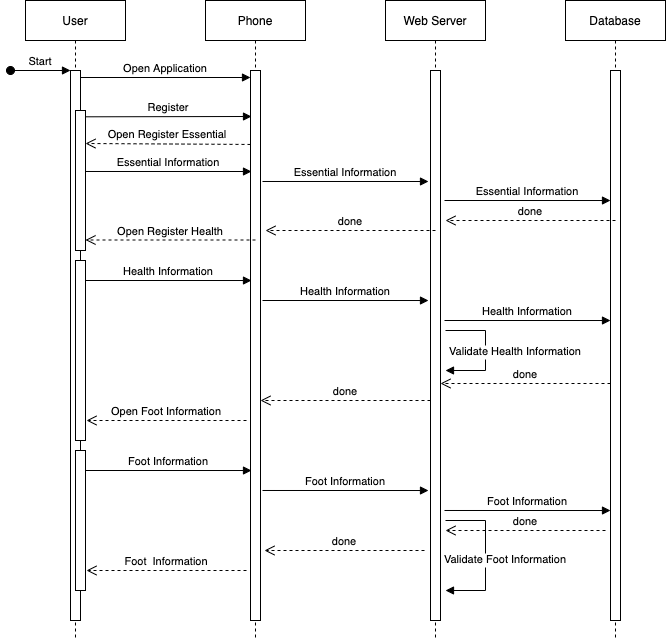
\includegraphics[width=.9\columnwidth]{KaanEksenMSc/figures/PredictionModuleSequenceDiagram.png}}
\caption{Prediction module sequence diagram}
\label{fig:PredictionModuleSequenceDiagram}
\end{figure}

In the prediction module, the collected information should also inform health professionals in order to reduce examination time. Besides that, in Section \ref{sec:FineTuneModule}, Fine Tune Module, the system performance improvement step, which is formed by adding new data to be obtained from health professionals, will be discussed.

In addition, all end-user applications should be user-friendly and provide sufficient feedback information for users. This feedback will improve user satisfaction and reduce the overall process's time consumption, such as application usage instructions.

Last but not least, the prediction module collects statistical data as part of the survey. Conducting surveys through the end-user applications will allow the system to reduce UI shortcomings. Apart from these, the same surveys will also enable healthcare professionals to receive feedback on actively performed healing procedures. Some procedures require users to perform actions on a daily or weekly basis. Therefore surveying these actions to improve users' overall experience on digital healthcare is of utmost importance for the system to be more user friendly.

\subsection{ Fine-Tune Module }\label{sec:FineTuneModule}

The fine-tuning module, which is the integral part, should include background procedures and healthcare professionals' interface. In order to achieve this, the module should implement two functionality namely system enhancement and user interface. Accordingly, in order to provide workflow, healthcare professionals, also known as system managers, should review and analyze user-provided data, which should be used to refine system diagnoses process. Eventually, the system should actively enhance the pre-diagnosis process by using the data doctored and adjusted by the system managers.

\begin{figure}[htbp]
\centering
\fbox{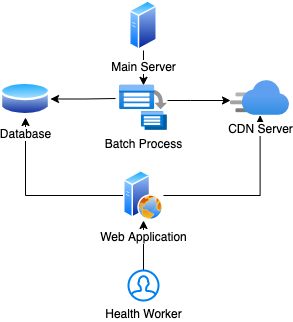
\includegraphics[width=.5\columnwidth]{figures/FineTuneModuleDiagram.png}}
\caption{Fine-tune module diagram}
\label{fig:FineTuneModuleDiagram}
\end{figure}

As can be seen in Figure \ref{fig:FineTuneModuleDiagram}, a web application should be implemented for system managers to display and review the user input, such as foot images, previous diseases. In the web application, system managers should be able to calculate foot types with objective measurement methods such as the Staheli arch index with provided images from the user. As a result of this calculation, there will be two results, one provided from the doctor, and one generated by the system which can be later compared.


System managers supply data in an orderly fashion in dual circles; provide, validate (see Figure \ref{fig:FineTuneModuleWebApplicationActivityDiagram}). Healthcare professionals view patient information in the provided cycle and contribute foot type detection inputs. Information viewing involves primary data (BMI, Shoe Size), patient complaints (pain level, pain duration), health history (surgeries and chronic diseases), and foot pictures. Afterward, foot type detection inputs are provided by health workers. As a result of detection inputs, the system should be able to calculate multiple foot indexes. In Figure \ref{fig:FineTuneModuleWebApplicationSequenceDiagram}, the sequence diagram of the fine-tune module can be seen.

\begin{figure}[htbp]
\centering
\fbox{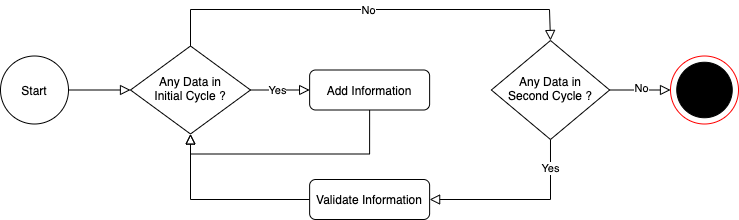
\includegraphics[width=.8\columnwidth]{figures/FineTuneModuleWebApplicationActivityDiagram.png}}
\caption{Fine-Tune Module - Web Application - Activity Diagram}
\label{fig:FineTuneModuleWebApplicationActivityDiagram}
\end{figure}

At the end of the initial cycle, the system should calculate well known accepted foot indexes using key points obtained from healthcare professionals. These indexes should be pre-defined such as Chippaux-Smirak Index, Arch Height Index.

\begin{figure}[htbp]
\centering
\fbox{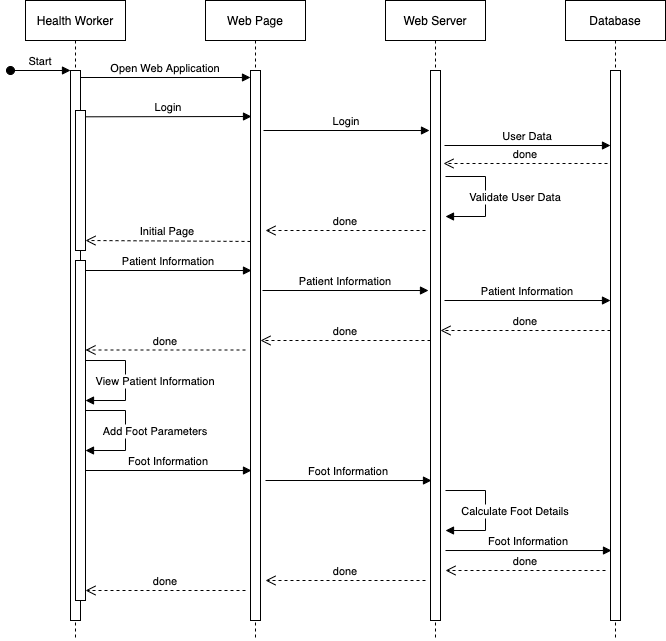
\includegraphics[width=.9\columnwidth]{figures/FineTuneModuleWebApplicationSequenceDiagram.png}}
\caption{Fine-tune module web application activity diagram}
\label{fig:FineTuneModuleWebApplicationSequenceDiagram}
\end{figure}

The second cycle should provide the calculated data to healthcare officials to validate the results. The system user should see how the results are calculated, related user data, and other meaningful information in this second cycle. At this stage healthcare professionals can respond to each of the results as move to initial cycle, unusable or approved. Accordingly, the approved results should be used to improve batch process performance

Furthermore, the second cycle should also focus on preventing any user-related errors. Therefore, multiple calculation results, formulas, and corresponding result statuses (pes planus and pes cavus) should be displayed to reduce the errors. In addition, the system should be able to rewind the cycle to the initial state is based on healthcare professionals' decisions.

\subsection{ Batch Process }

The batch process should be designed to improve the pre-diagnosis with the data provided from the prediction and fine-tune module. In addition, the batch process should be automated for continuous learning. Therefore, this will provide the system to improve itself over time through the data provided by the modules (doctors and patients). 

\begin{figure}[htbp]
\centering
\fbox{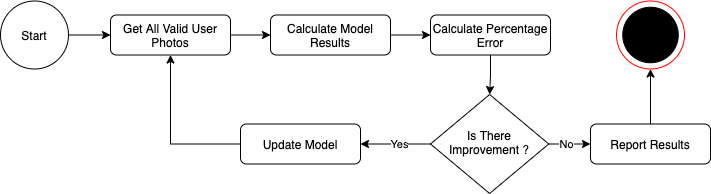
\includegraphics[width=.9\columnwidth]{figures/BatchProcessActivityDiagram.png}}
\caption{Batch process activity diagram}
\label{fig:BatchProcessActivityDiagram}
\end{figure}

The batch process should consist of four basic steps. Firstly, the batch process should get all the valid user-provided photos from the prediction module. Then, the system should process all the images on the current model and calculate the results. After the calculation, the batch process should calculate percentage errors with provided data from healthcare professionals. Then, based on results improvements, the model is updated or not. Finally, all the calculations should be redone when the model is updated until the best results are obtained. In Figure \ref{fig:BatchProcessActivityDiagram}, the activity diagram of the batch process can be seen.

In addition, the batch process should provide reports about the system's detailed and overview progress, which contains calculated multiple errors. The overview results are a comparison of patients' diagnoses. As a result, this error calculation should provide how successful the system is as a product. Moreover, the detailed error results should be used to improve the system in short cycles. The detailed error calculation should use sub-findings of the system and the calculation points provided by health workers, such as points on the pictures used to identify foot structure. 

\subsection{ Foot Index Calculations }

The system should use multiple methods to find the best approach and assist healthcare professionals in diagnosing patients successfully. Therefore, a fine-tune module system should provide foot indexes, calculation methods used in the examination such as Arch Height Index, Chippaux-Smirak Index, Staheli Index, Clarkes Angle Calculation, Rearfoot Angle Calculation. 

Each calculation type requires its specialty to diagnose accurately, such as the calculation of specific angles of the foot structure. Therefore, the system focuses on a specific type of index calculation, the Arch Height Index, in an automated process to reduce errors.

The arch height index should be calculated using a single foot image. Thus single image usage reduces user workload and improves user experience. In addition, the arch height index requires an image of the foot containing the side of the foot to calculate the index type correctly. This image should be used to detect reference points on the side of the foot. 

Other index calculations are not used for the automated process. They were used only with the data provided by healthcare professionals, which details are explained in the offline phase part. Instead, other index methods are used as reference methods for our calculations. This will allow us to compare different types of measurements. Consequently, the best method for the mobile approach will be selected. The calculation details can be seen in Chapter \ref{chp:Methodology}.

\section{IMPLEMENTATION}\label{sec:StudyIImplementation}

This section discusses the implementation details and decisions of the study. The study contains multiple applications. Each application is divided into its implementation section. In addition, this section starts with the development process subsection, which explains applied development processes for each application.

\subsection{Development Process}

Software engineering is one of the fastest-growing fields in computer science. Over the years, it has had some milestones in development processes. However, in general, iterative development in its core has never changed. The most significant difference in software development processes is the reaction to changes in requirements. Therefore,  a hybrid model of software development processes is applied, which are different in each application. This section will provide information regarding this decision and the reasons for it.

Client applications follow the prototype development process since collecting the data was crucial at the start of the development process. In addition, client applications contain dynamic composition where requirements change based on feedback. For example, only the iOS operating system was supported at the beginning of the project, but the Android prototype was also introduced due to the diverse mobile market and the users' need for Android applications.

On the other hand, batch processes, which used by the other application in Study I, were less prone to change and had no different types. Therefore, the waterfall development process is adopted. In addition, the server APIs for rapid response to client application changes have continuously improved throughout its lifetime as it fundamentally embraces Agile development.

\subsection{End-User Application}

The end-user system contains two distinct clients, which are iOS and Android. Client applications developed in mind usability, accessibility, inclusion, updated and improved during the application lifecycle. Consequently, this will improve the user experience and be satisfactory for all user groups.

The iOS client is compatible with iOS 11 and forward, making it accessible for 99,7 percent of the market share. Furthermore, mainly Swift programming language is used for the development of the client. Therefore, this makes it easy to support feature updates and compatibility for all the iOS ecosystems. 

\begin{figure}[htbp]
\centering
\fbox{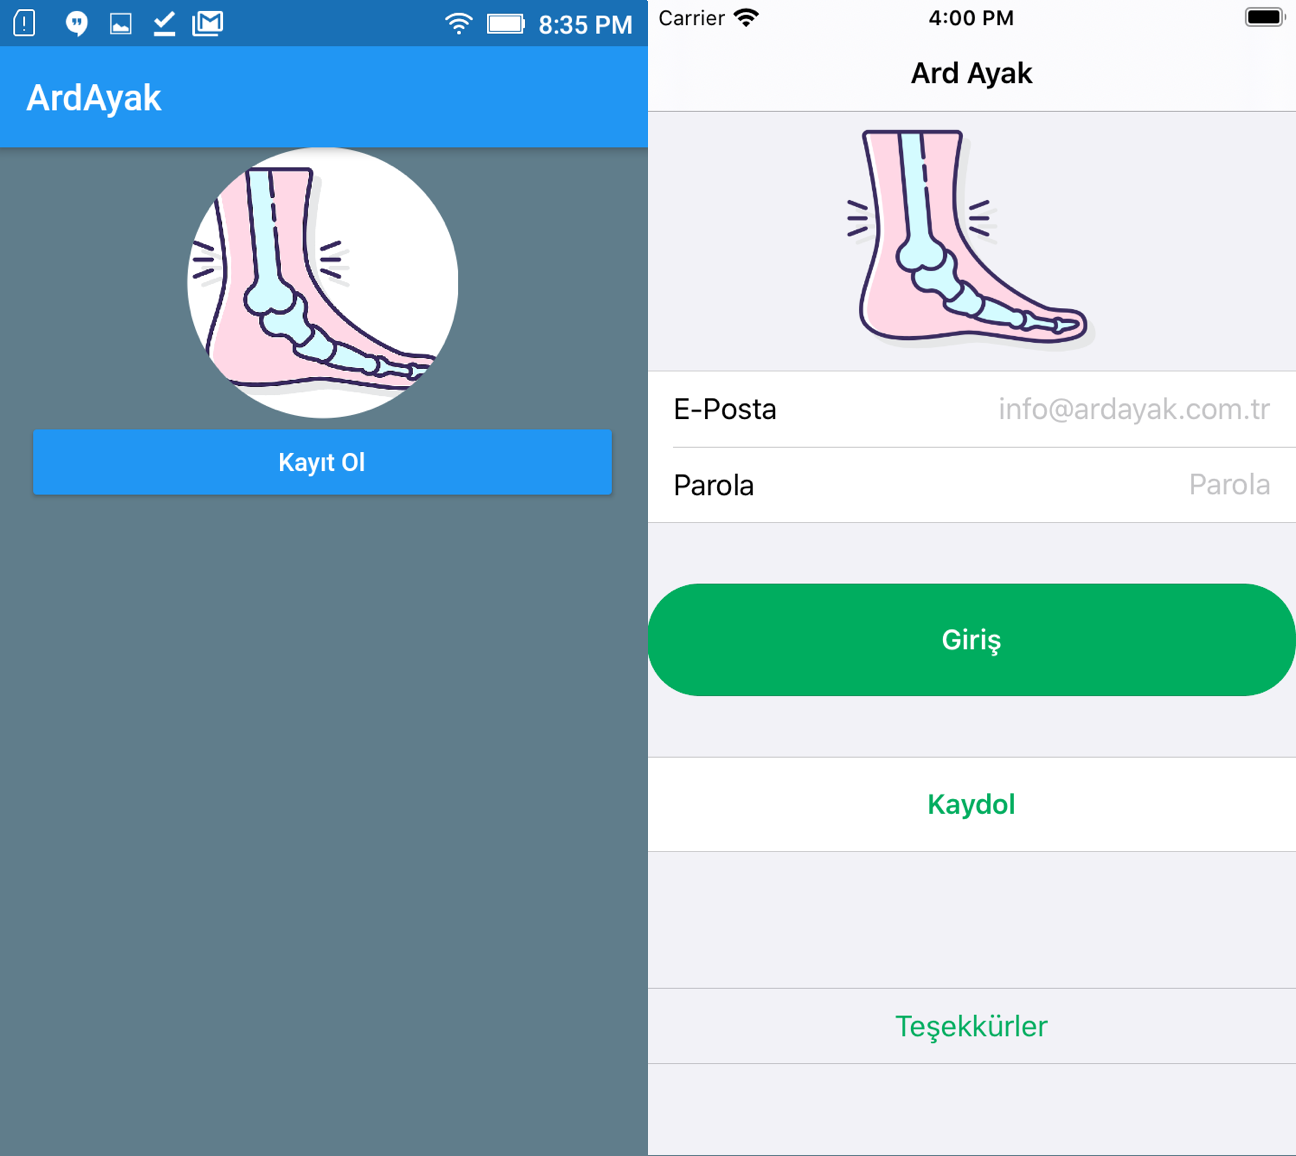
\includegraphics[width=.7\columnwidth]{figures/UserApplicationUI.png}}
\caption{Android (left) and iOS (right) application UI}
\label{fig:UserApplicationUI}
\end{figure}

The Android client is compatible with API level 16 and forward, making it accessible for 99,8 percent of the market share. Furthermore, the Flutter software development kit is used in the development process, which requires Dart programming language. Therefore, this makes the software compatible with iOS and Android publishing. On the other hand, the Flutter application is only used for Android clients as this process requires additional development. However, this feature can also be used in the future development process to reduce development costs.

Both end-user applications use the same user flow with corresponding platform UI specifications. Therefore this will enable users to complete their operations more comfortably with the UI they frequently use, shown in Figure \ref{fig:UserApplicationUI}. Furthermore, user documentation is also created to help smooth the user experience. This document contains all the information, from how to use it to the download links of the application. 

\begin{figure}[htbp]
\centering
\fbox{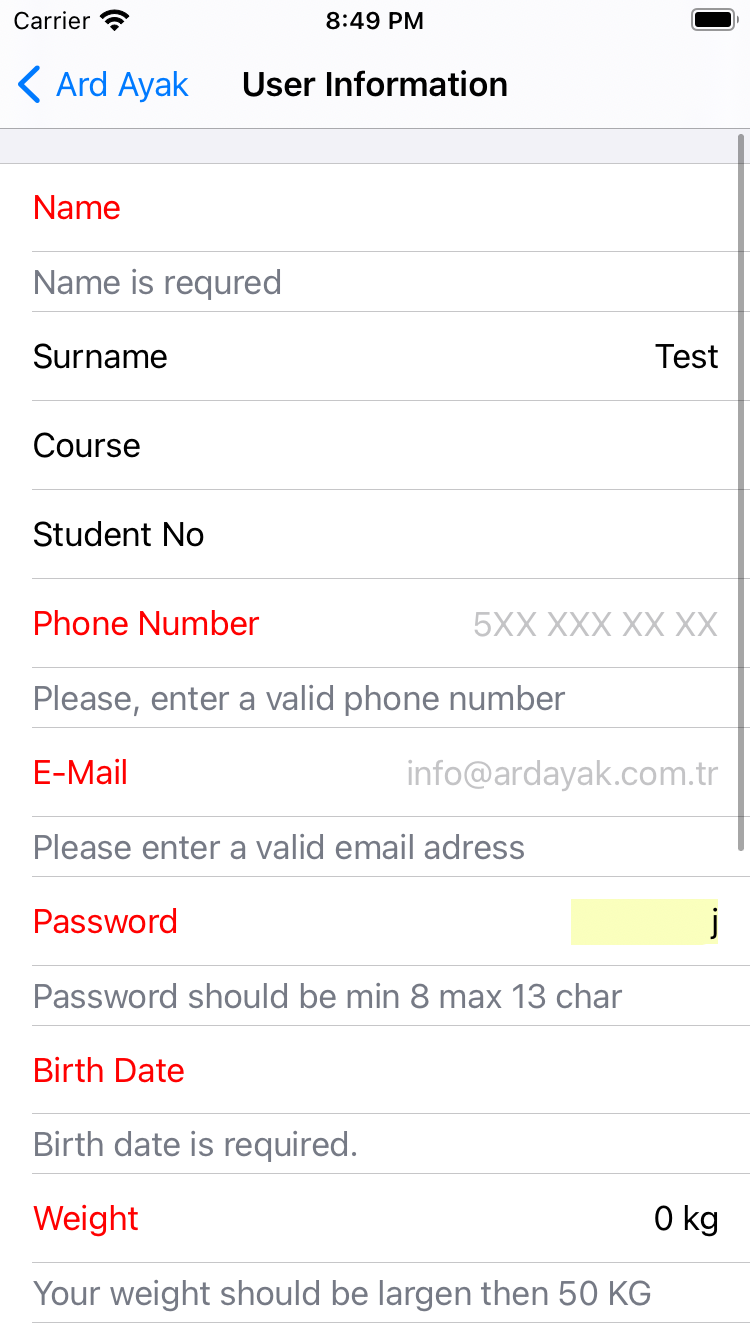
\includegraphics[width=.4\columnwidth]{KaanEksenMSc/figures/UserApplicationValidations.png}}
\caption{User application validations (iOS)}
\label{fig:UserApplicationValidations}
\end{figure}

Even though end-user documentation is created, client applications always consider user mistakes and misunderstandings. Therefore, input validation and feedback are implemented through the application. These validations include input type, max-min character, logical validations, and many more, shown in Figure \ref{fig:UserApplicationValidations}, to improve users' experience. In addition, user tutorials are also added to guide the user, which is shown in Figure \ref{fig:UserApplicationOnboarding}.

The image collection is a fundamentally similar process for both clients. This process includes taking a photo or taking it from the gallery. After that, since image sizes would be different in different hardware, iOS and Android prototype applications resizes the image and transfer it in base64 format. Furthermore, file compression is used to reduce the traffic when transmitting the images from client to server. Deflate, a lossless compression format, is selected for compassion since it is a widely used open-source compression algorithm available in major operating systems. In addition, there is a file format validation on clients for gallery-selected images. 

\begin{figure}[htbp]
\centering
\fbox{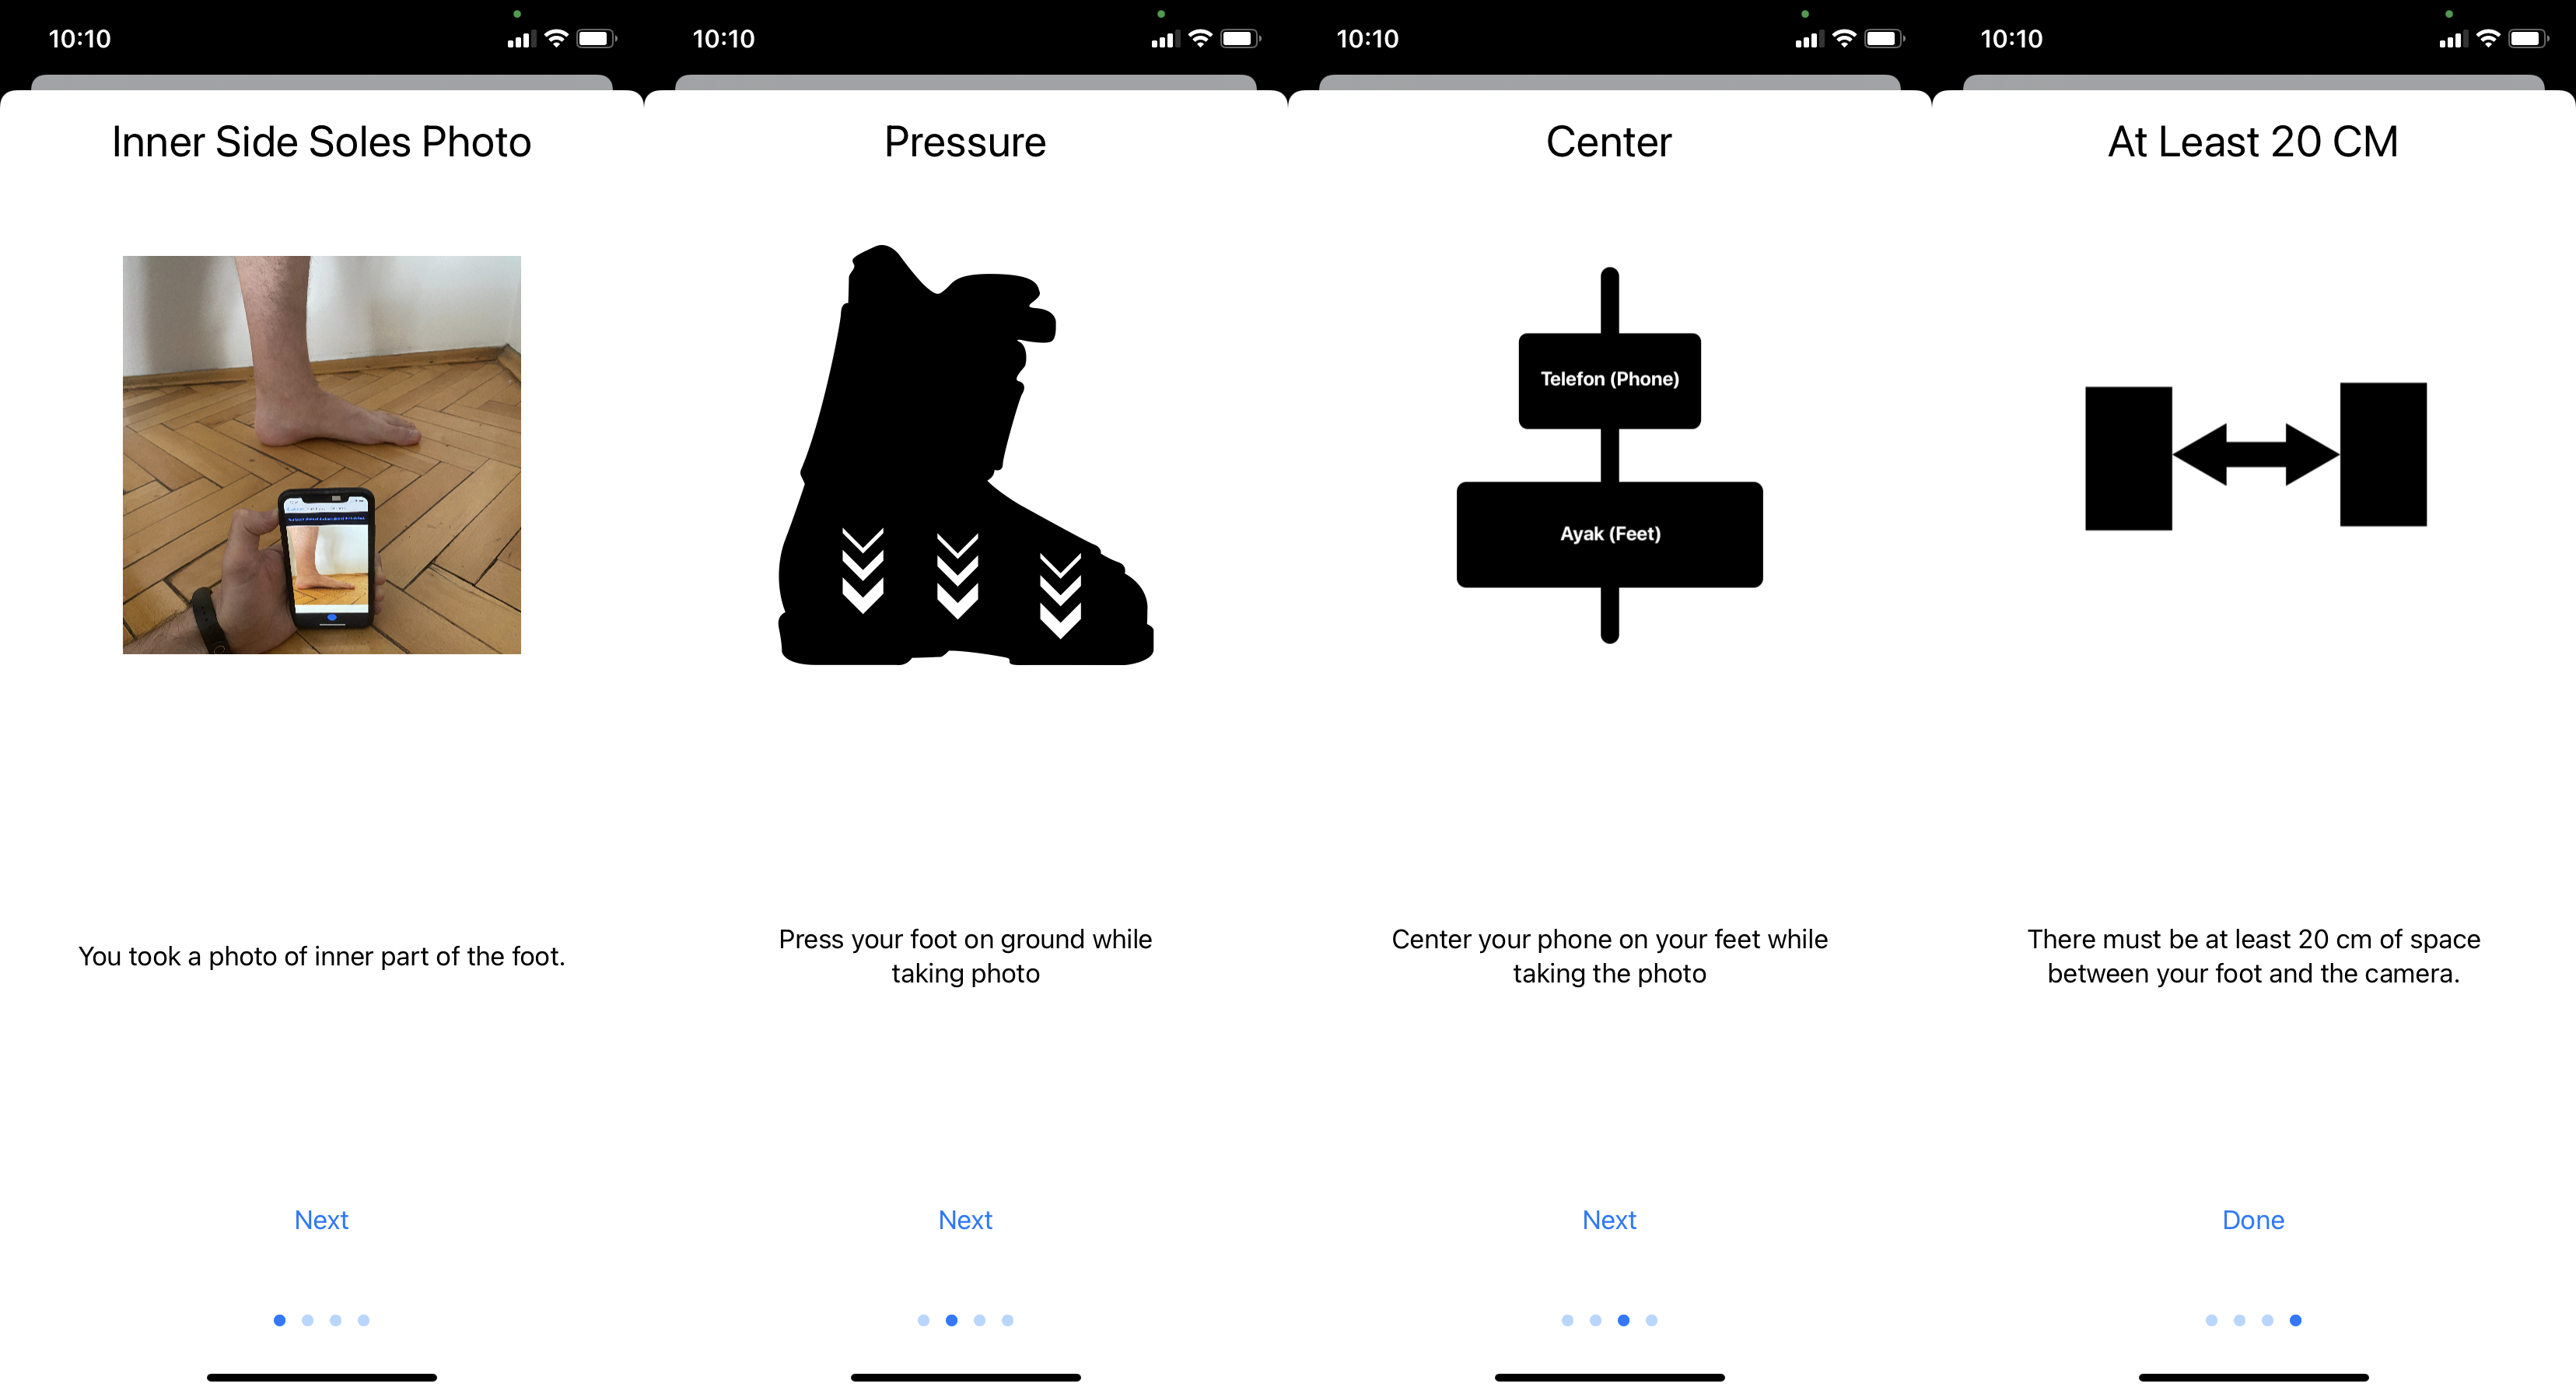
\includegraphics[width=.9\columnwidth]{KaanEksenMSc/figures/UserApplicationOnboarding.png}}
\caption{User application onboarding (iOS)}
\label{fig:UserApplicationOnboarding}
\end{figure}

The shooting angle and feet pressuring the ground during the photos shooting are essential for pes planus and pes cavus detection. Therefore onboarding is displayed (see Figure \ref{fig:UserApplicationOnboarding}) before each shooting. This onboarding shows a preview of how shooting should be and the state of the foot. As a result, this will reduce human-related errors furthermore. 

\begin{figure}[htbp]
\centering
\fbox{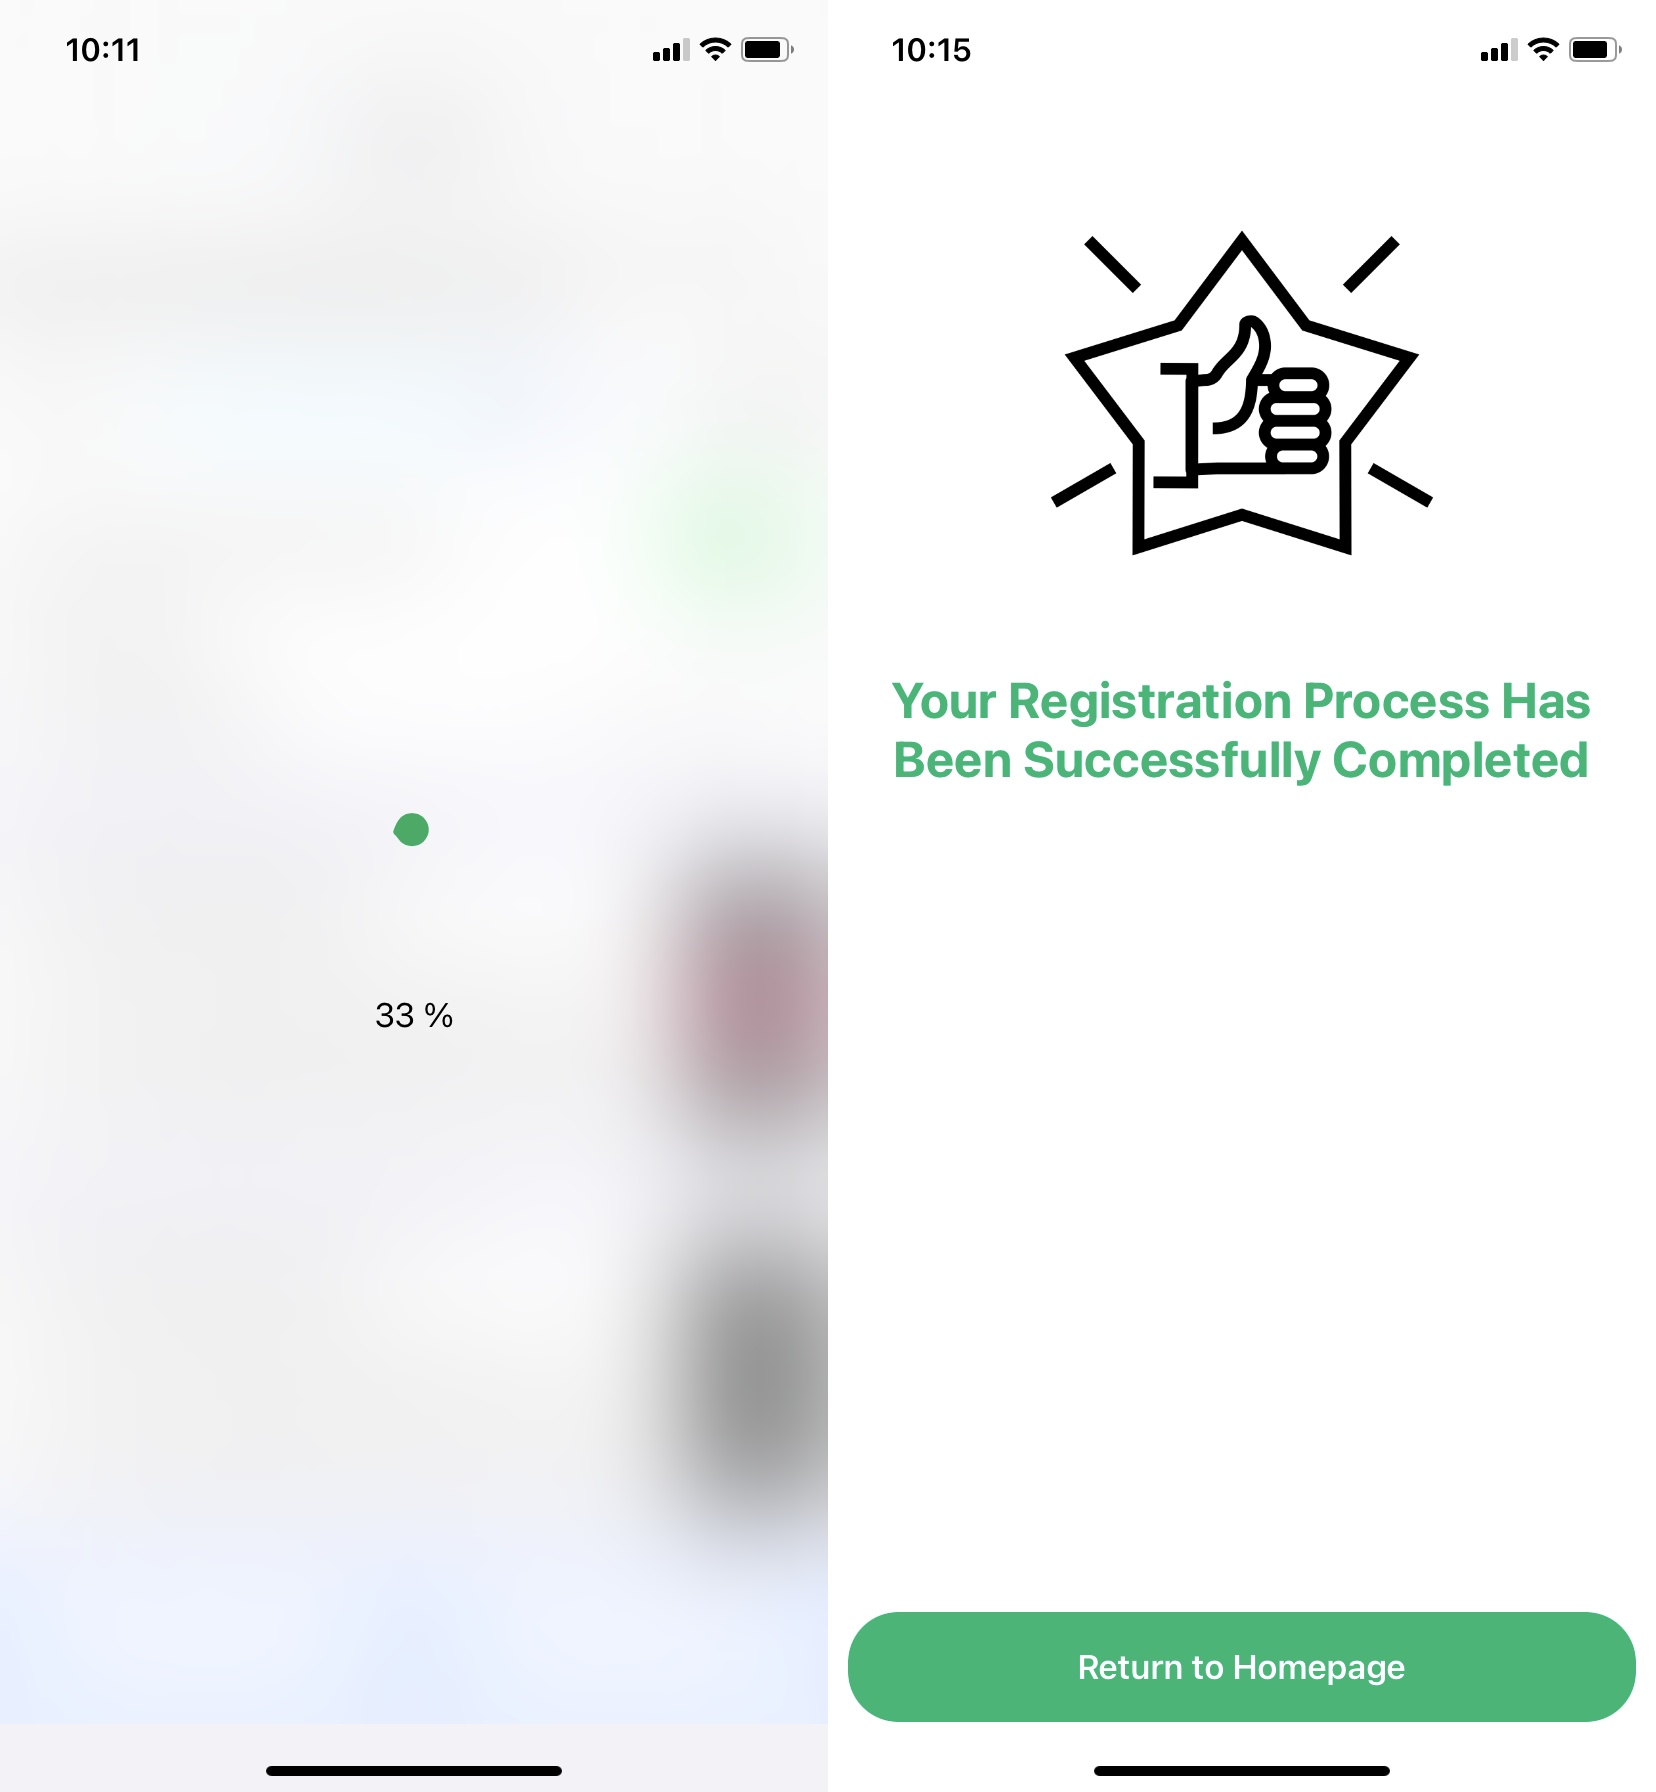
\includegraphics[width=.6\columnwidth]{figures/UserApplicationFeedback.png}}
\caption{User application feedback (iOS)}
\label{fig:UserApplicationFeedback}
\end{figure}

Feedbacks are one of the most critical aspects of the user experience. Therefore, multiple feedback mechanisms are developed in client applications to reduce communication errors. For example, since image uploading relatively takes more time than the other operations in the application, a progress bar with percentages is developed (see Figure \ref{fig:UserApplicationFeedback}). In addition, success screens are developed to indicate to users that the process is completed (see Figure \ref{fig:UserApplicationFeedback}).

The most important difference between iOS and Android processors is that some mobile phone models provide information other than raw image data during photo capture. For example, some of the Apple hardware contains LIDAR sensors. Therefore, the iOS client uses this hardware advantage and sends extra information to the service, which is the depth data. This depth information could be used to increase the accuracy of pre-diagnosis. In addition, depth data is converted to Point Cloud Data format before being transferred to the server for future updates for other systems.

Lastly, localization is one of the features of the client applications. Applications support multiple languages to increase usability in multiple regions in the world. In addition, supporting other languages would be straightforward as adding a new file to the application language file base. Furthermore, the client applications use operating system APIs to open the application in users' preferred language.

\subsection{Specialist Interface} \label{sec:SpecialistInterface}

The specialist interface is a web application whose primary purpose is to enable healthcare professionals to view patient data and diagnosis the patient based on the provided data. In the background, this process also improves the system by providing data to improve pre-diagnosis, which will be detailly discussed in the batch process. 

\begin{figure}[htbp]
\centering
\fbox{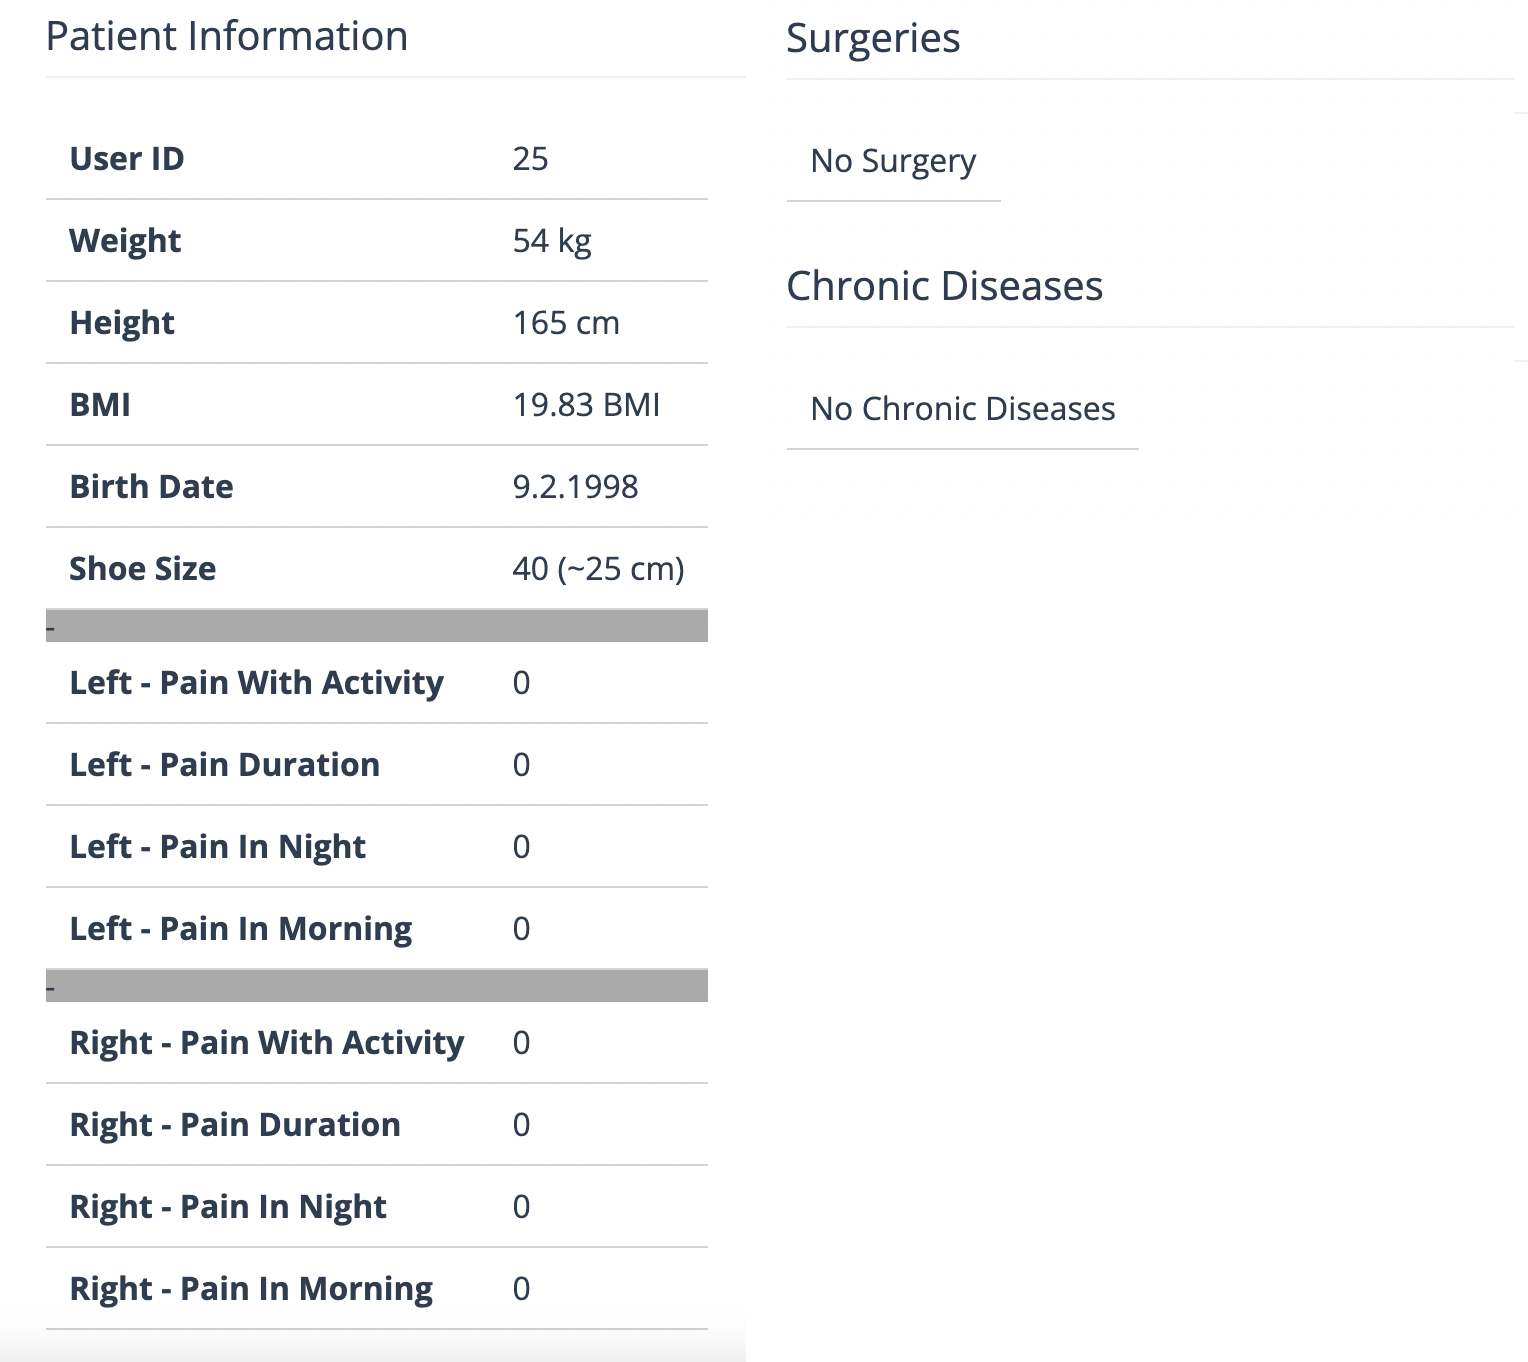
\includegraphics[width=.8\columnwidth]{figures/WebApplicationPatientInfo.png}}
\caption{Web application patient information}
\label{fig:WebApplicationPatientInfo}
\end{figure}

The specialist interface is designed to work in two cycles. In the first cycle, the system provides essential patient information such as age, foot size, surgeries, and chronic disease, shown in Figure \ref{fig:WebApplicationPatientInfo}. After validating initial information, healthcare professionals can set key decision-making points in images provided by patients, which will be used to calculate novel-approved foot indexes. 

\begin{figure}[htbp]
\centering
\fbox{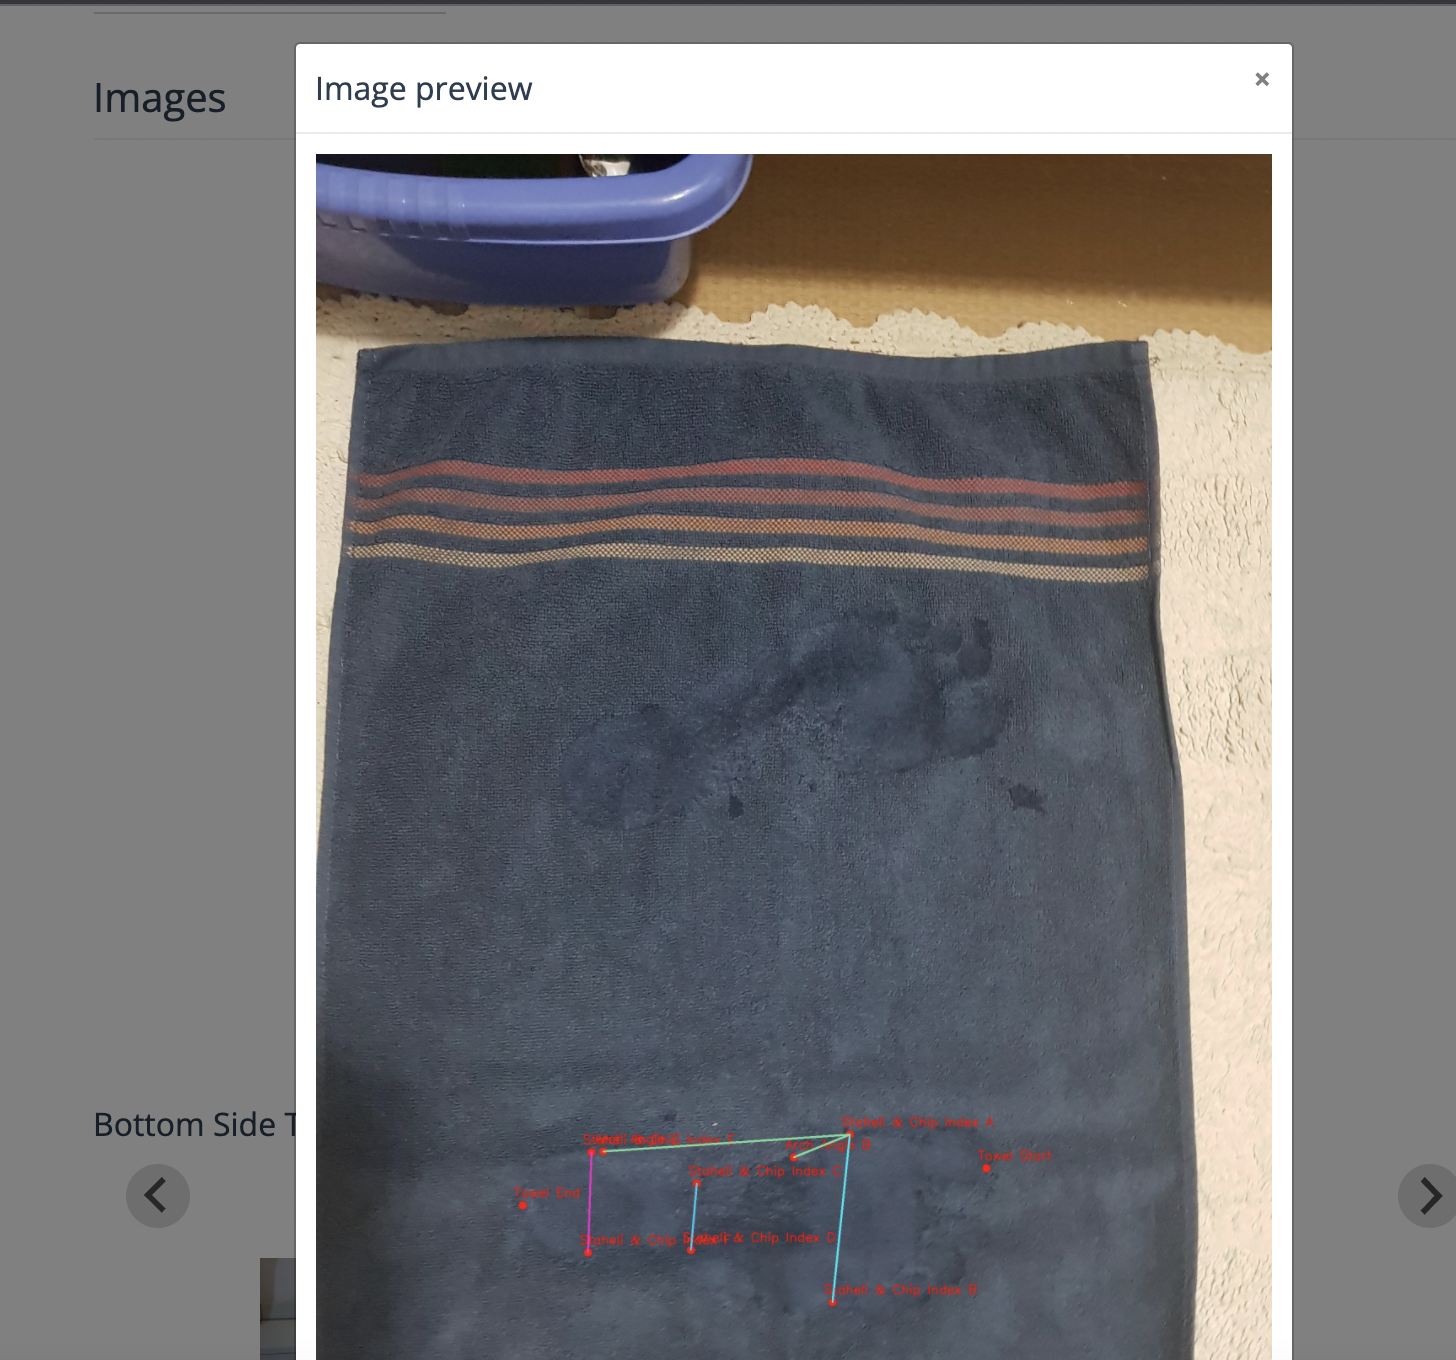
\includegraphics[width=.8\columnwidth]{KaanEksenMSc/figures/WebApplicationFootPoints.png}}
\caption{Web application critical foot points on image}
\label{fig:WebApplicationFootPoints}
\end{figure}

\begin{figure}[htbp]
\centering
\fbox{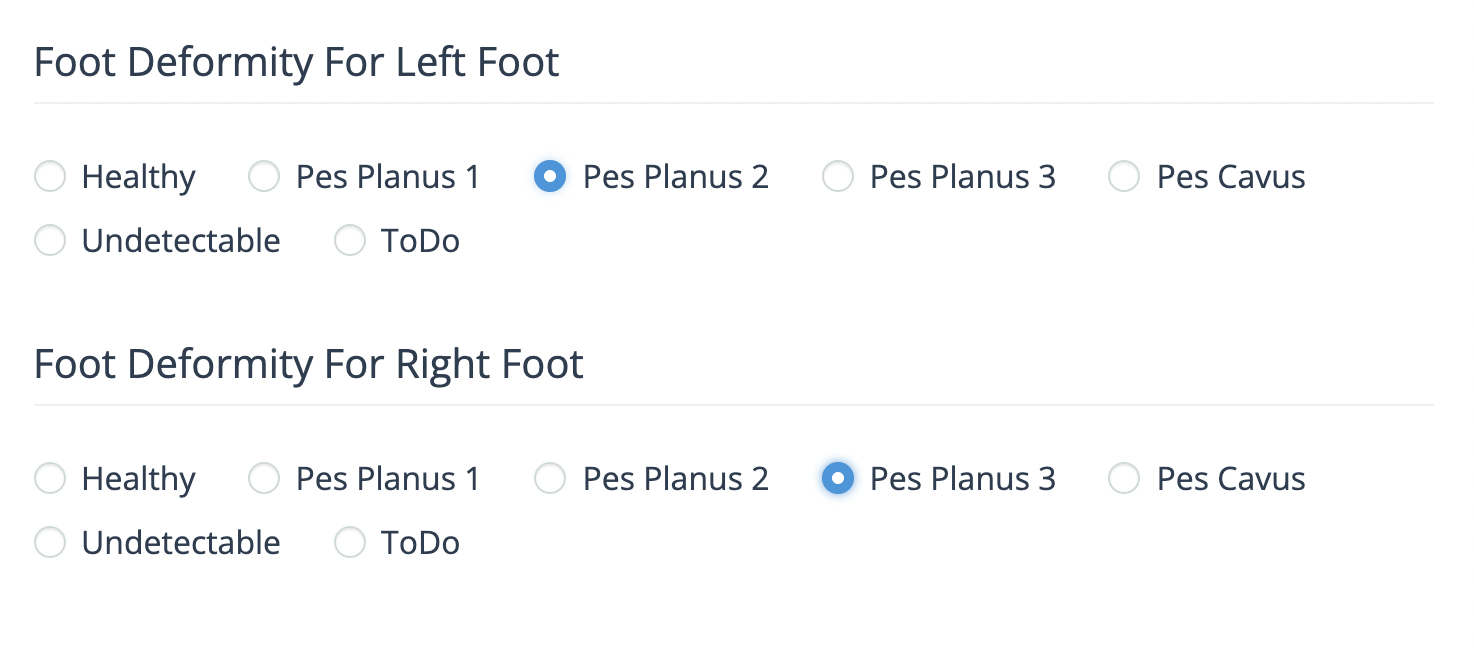
\includegraphics[width=.9\columnwidth]{KaanEksenMSc/figures/WebApplicationSetFootDeformity.png}}
\caption{Web application foot deformity options}
\label{fig:WebApplicationSetFootDeformity}
\end{figure}

The second cycle provides calculated results so that healthcare officials can make the final diagnosis of the patient's condition. Therefore, applications provide an overview of the patient information and display decision-making points in images to ensure they are correct (see Figure \ref{fig:WebApplicationFootPoints}). Healthcare officials can redo the point set or diagnose the patient (see Figure \ref{fig:WebApplicationSetFootDeformity}). In addition, in case of unusable images, there is an option that asks the user to re-upload foot pictures.

\begin{figure}[htbp]
\centering
\fbox{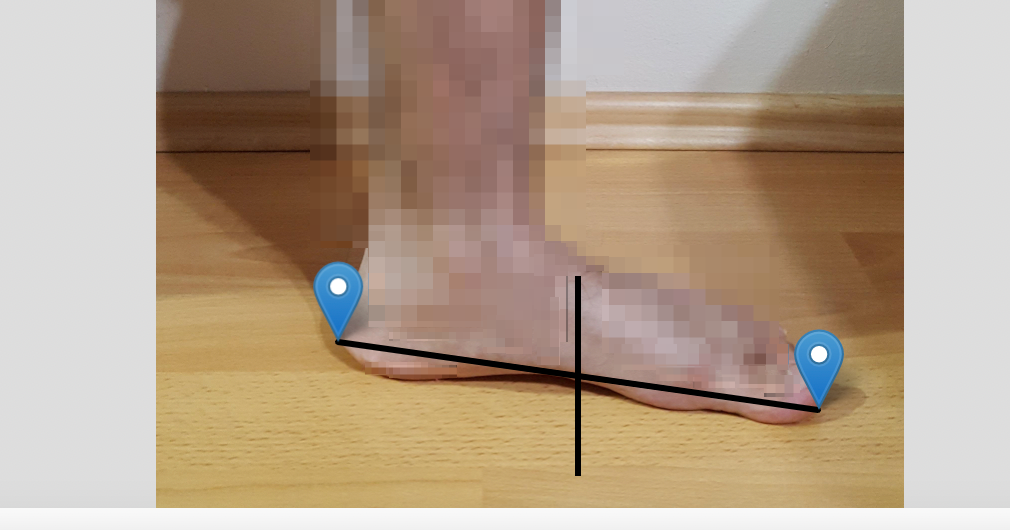
\includegraphics[width=.6\columnwidth]{KaanEksenMSc/figures/WebApplicationCriticalPointAssistance.png}}
\caption{Web application critical point assistance}
\label{fig:WebApplicationCriticalPointAssistance}
\end{figure}

The web application contains validations to ensure current diagnosis. Thus, the system ensures that all the critical points are set in the initial cycle. The second cycle provides that human-related errors are eliminated, such as wrongly placed points. 

\begin{figure}[htbp]
\centering
\fbox{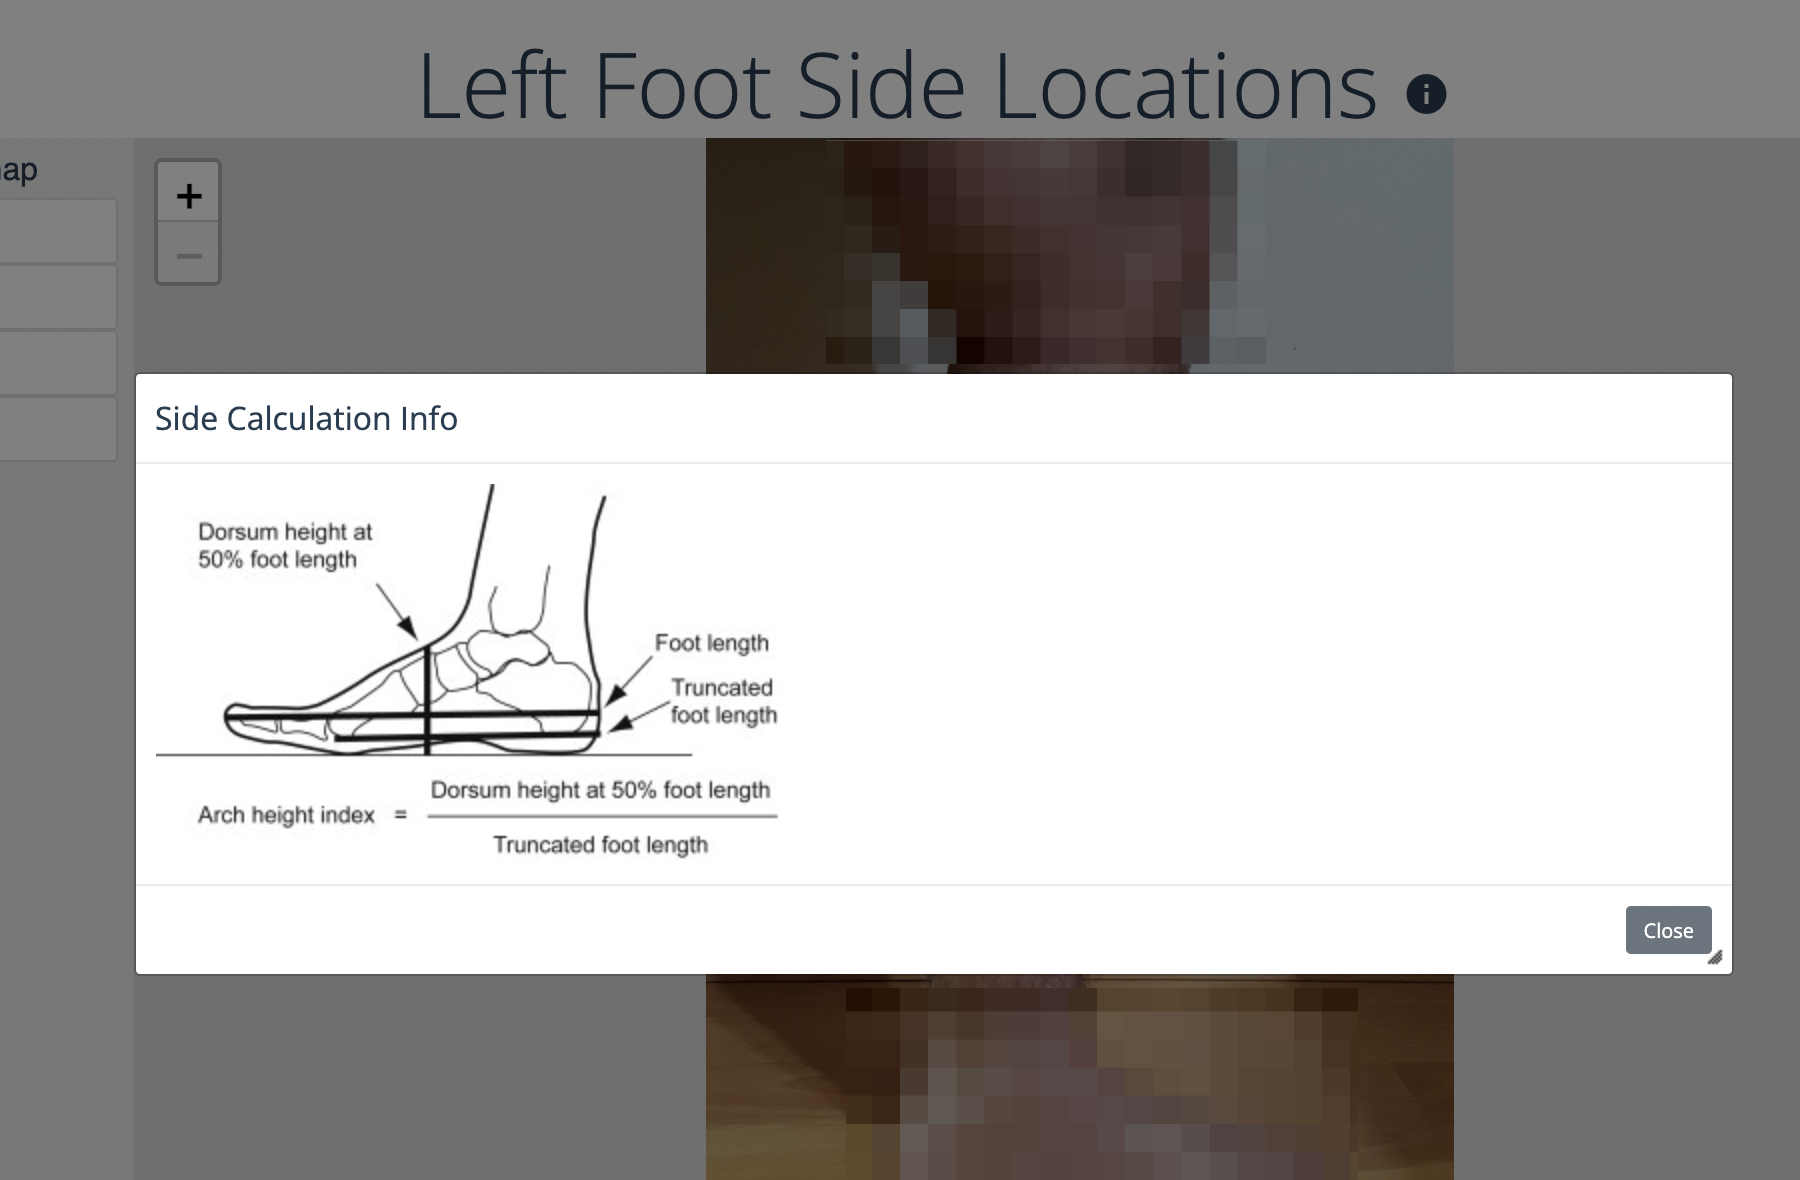
\includegraphics[width=.6\columnwidth]{KaanEksenMSc/figures/WebApplicationInformationBoxes.png}}
\caption{Web application information boxes}
\label{fig:WebApplicationInformationBoxes}
\end{figure}

In addition, The web application also provides helper functionalities to healthcare workers such as critical point assistance and information boxes. For example, the arch height index requires finding the center of the points therefore the critical point assistance displays (see Figure \ref{fig:WebApplicationCriticalPointAssistance}) the center of the points provided by the health professionals. Another example is that information boxes provide simple reminders about indexes (see Figure \ref{fig:WebApplicationInformationBoxes}).

\subsection{Services And Batch Process} \label{sec:StudyIServicesAndBatchProcess}
The application consists of two services: web and client application service. This structure provides scalability and security. Therefore, one service deals with end-user interactions and data transmission. At the same time, web service provides healthcare professionals and batch processes. With this separation, each service is placed in different layers. Therefore, this makes it possible that only client application services have internet access, increasing the web application security by limiting internet access. In addition, this will provide more hardware-intensive operations (image processing, deep learning) to other physical servers. 

Client application services adopt the microservice architecture for scalability and respond quickly to requirements. Furthermore, to prevent unauthorized access JWT (RFC 7519) is used. Lastly, all communications have been done by HTTP protocol with an SSL (RFC 6101). 

The batch process is the system's core, where the pre-diagnosis is done. The pre-diagnosis computation has three main steps: finding the region of interest, image pre-processing, and detection. Afterward, results are shared with the appropriate application and recorded in the database. In the following paragraphs, each step is detailly explained.

The initial step requires finding the foot in the image, also called the region of interest (ROI). Since all the data is collected unsupervised, the foot can be anywhere in the image. Therefore, roughly locating the foot for detail processing is essential. Deep learning algorithms are excellent in object recognition, but they require a vast amount of data to achieve this type of accuracy, so using deep learning algorithms for pre-diagnosis is close to impossible with the current dataset. As a result, the study uses pre-trained deep learning human detection algorithms to get a rough location of the foot.

\begin{figure}[htbp]
\centering
\fbox{\includegraphics[width=.7\columnwidth]{KaanEksenMSc/figures/DeepLearningTest.jpeg}}
\caption{Deep learning test - DeepLab, FCN, YOLO, Skin, MIDAS (left to right)}
\label{fig:DeepLearningTest}
\end{figure}

The foot detection rate of the algorithms might not be as accredited as the announced results because most public datasets contain an entire human body other than a barefoot. Therefore, multiple deep learning networks such as YOLO, MIDAS, FCN Resnet 101, DeepLabV3 have been tested in small datasets for best results (see Figure \ref{fig:DeepLearningTest}).

\begin{figure}[htbp]
\centering
\fbox{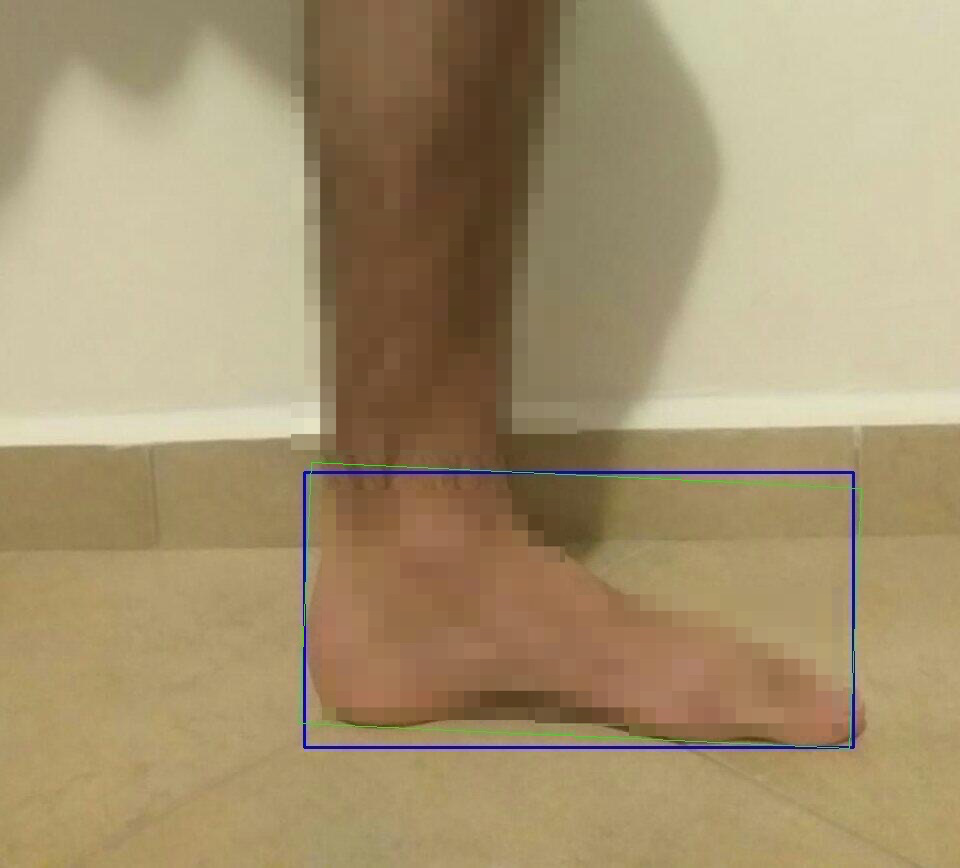
\includegraphics[width=.6\columnwidth]{KaanEksenMSc/figures/BatchProcessMinimumBoundingBox.png}}
\caption{Batch process minimum bounding box (green line)}
\label{fig:BatchProcessMinimumBoundingBox}
\end{figure}

In addition, skin detection algorithms are also tested. Initially, the YCbCr color space-based skin detection algorithm was applied, but detection results have been unsuccessful in some lighting conditions. Therefore, the zero-sum game-based skin detection algorithm proposed by Dahmani et al. \cite{dahmani2020zero} is also tested (see Figure \ref{fig:DeepLearningTest}). Overall, the best performance is achieved by DeepLabV3.

The second step deals with image preparation. After potential barefoot is detected, a minimum area rectangle is calculated because the foot's location and angle might not be as accurate as demonstrated in the usage document. Therefore, perspective transformation is applied with the minimum area rectangle, eliminating potential angle problems (see Figure \ref{fig:BatchProcessMinimumBoundingBox}). In addition, this will move any foot on the image to the left corner of the image, which will ease the calculations.

\begin{figure}[htbp]
\centering
\fbox{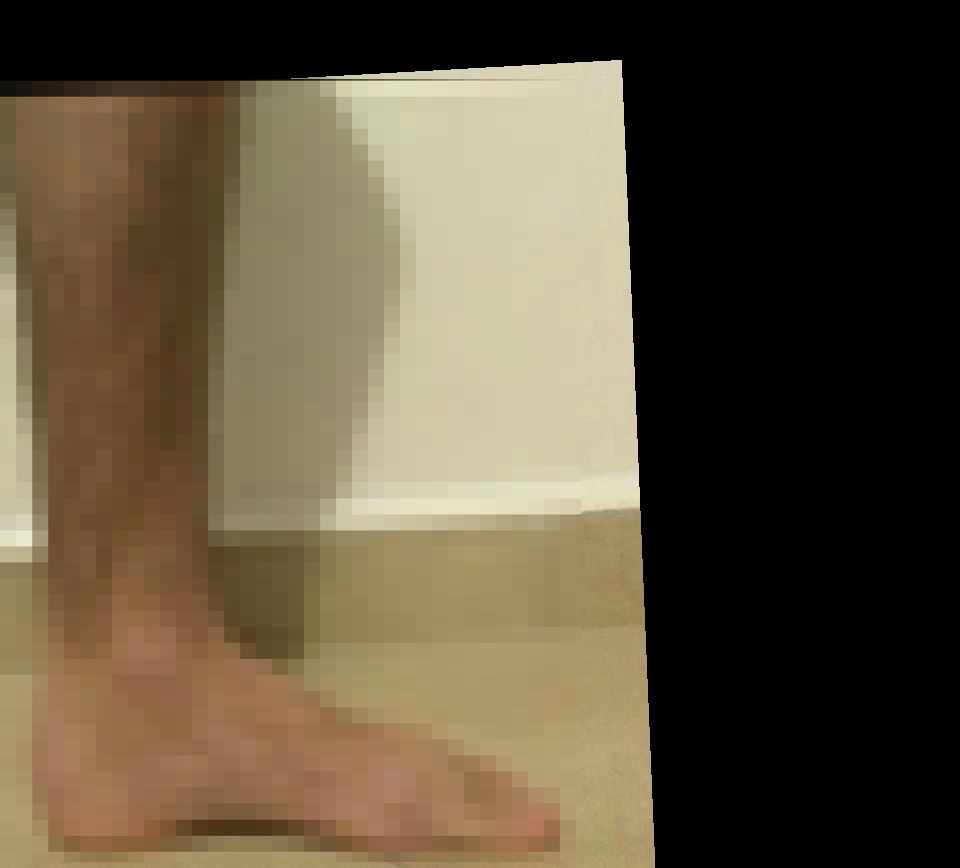
\includegraphics[width=.6\columnwidth]{KaanEksenMSc/figures/BatchProcessPerspectiveTransformation.png}}
\caption{Batch process perspective transformation}
\label{fig:BatchProcessPerspectiveTransformation}
\end{figure}

After the perspective transformation (see Figure \ref{fig:BatchProcessPerspectiveTransformation}), grayscale is required for edge detection algorithms. Therefore, RGB color space is converted to HSL because HSL has a separate lightness channel that can be eliminated. After all, lightness is unrelated to foot detection. The S channel was selected for the grayscale conversation since S performed better than H in the small dataset.

\begin{figure}[htbp]
\centering
\fbox{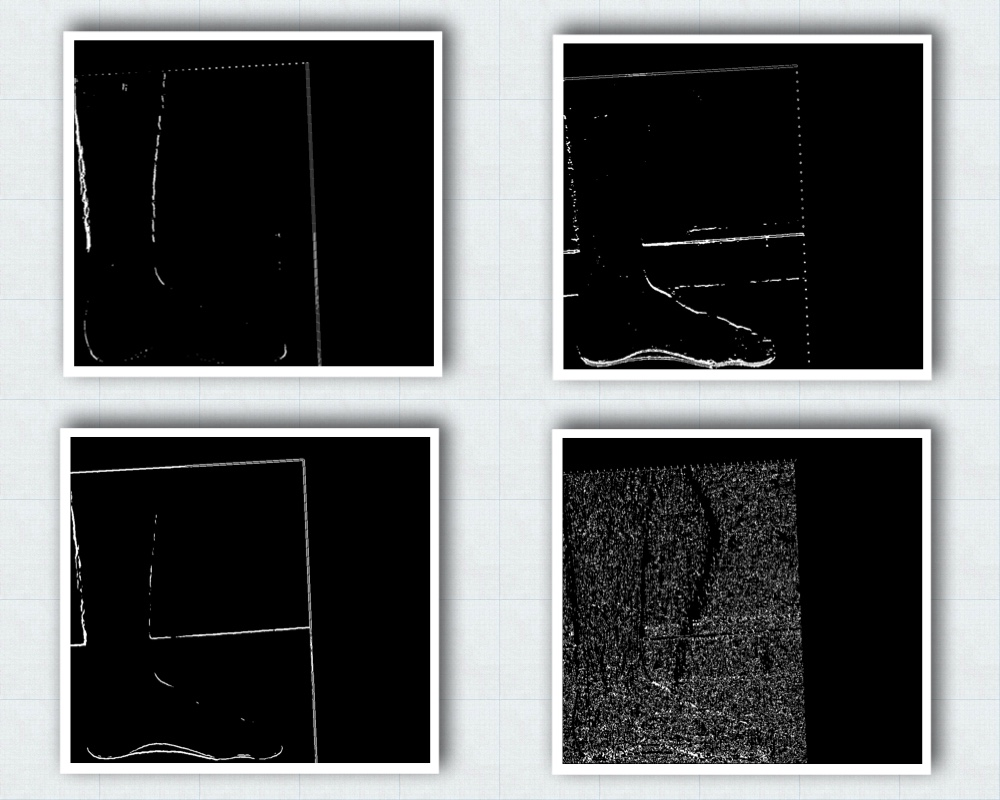
\includegraphics[width=.6\columnwidth]{KaanEksenMSc/figures/BatchProcessSobelOutput.jpg}}
\caption{Batch Process - Sobel - Absolute Gradient X, Absolute Gradient Y, Magnitude Gradient, Directional Gradient - Left To Right}
\label{fig:BatchProcessSobelOutput}
\end{figure}

The final stage includes edge detection and functionalization of the sole. The sobel algorithm is selected for edge detection with four different approaches with threshold values (see Figure \ref{fig:BatchProcessSobelOutput});

\begin{itemize}
  \item Applying an absolute gradient with the X direction
  \item Applying an absolute gradient with the Y direction
  \item Applying a magnitude gradient
  \item Applying a directional gradient with an angle threshold 
\end{itemize}

\begin{figure}[htbp]
\centering
\fbox{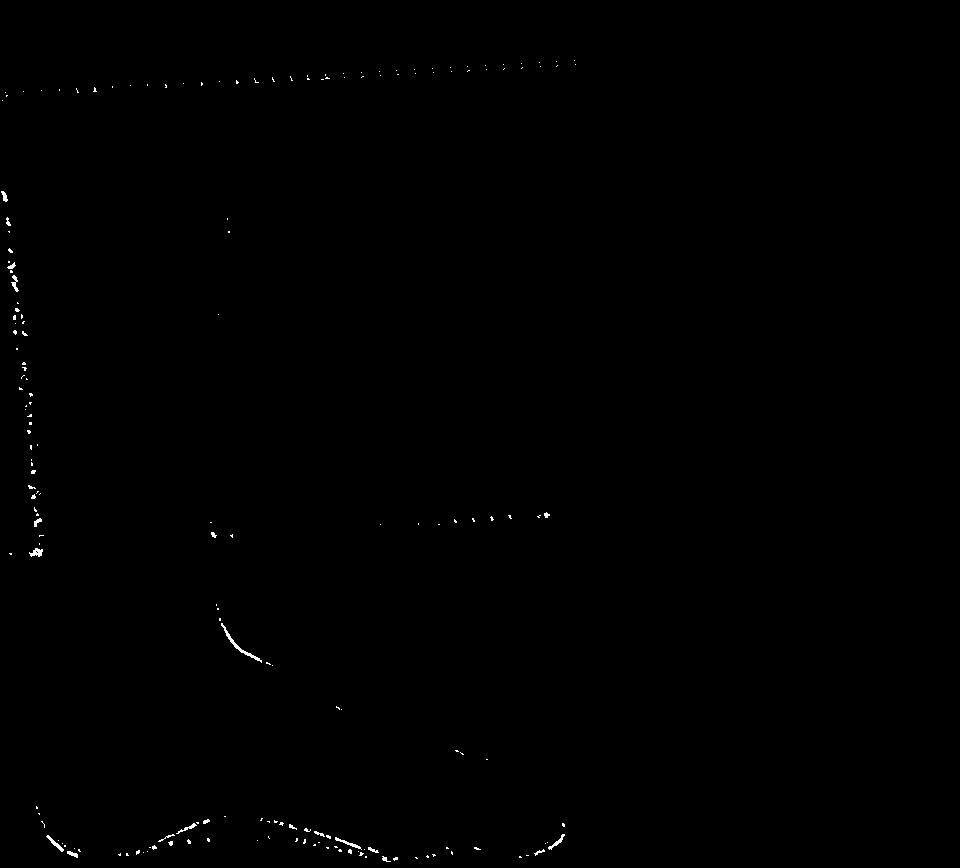
\includegraphics[width=.6\columnwidth]{KaanEksenMSc/figures/BatchProcessEdge.jpeg}}
\caption{Batch process Sobel combined}
\label{fig:BatchProcessEdge}
\end{figure}

After applying each configuration to the transformed image, results are merged into one with the algorithm \ref{alg:CombinedSobelResults}, which reduces unwanted pixels (see Figure \ref{fig:BatchProcessEdge}). 

\begin{figure}[htbp]
\centering
\fbox{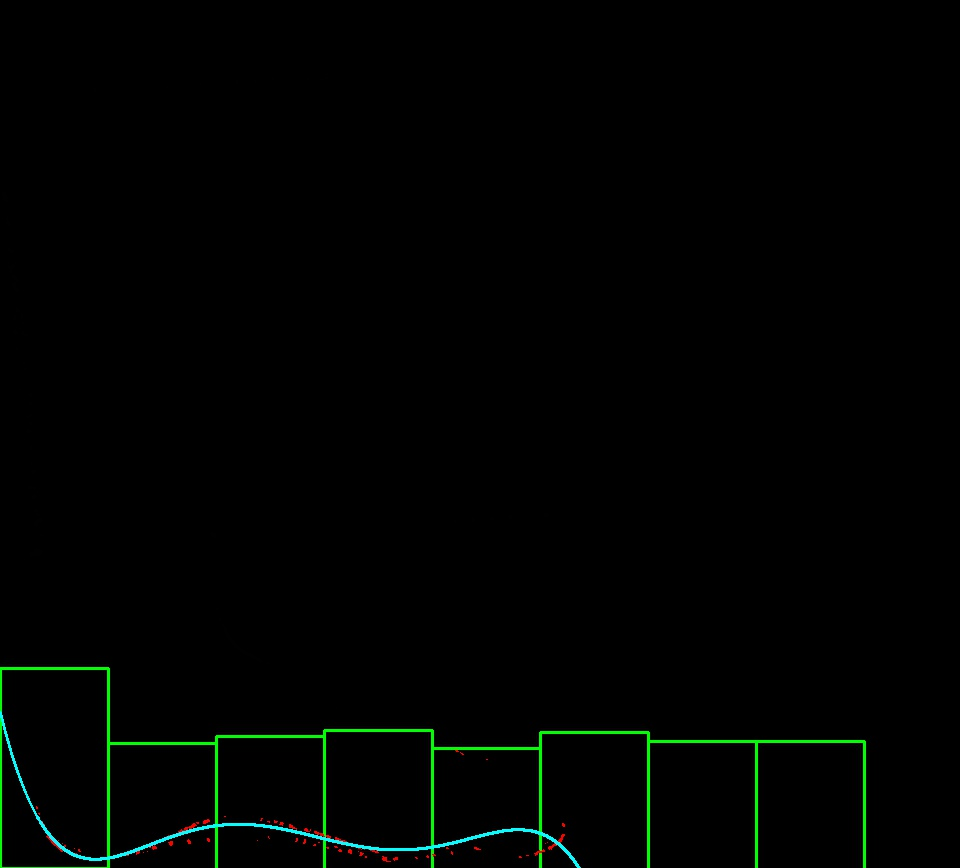
\includegraphics[width=.6\columnwidth]{KaanEksenMSc/figures/BatchProcessLine.jpeg}}
\caption{Batch process polynomial function}
\label{fig:BatchProcessLine}
\end{figure}

After the edges are extracted, polynomial regression is applied to generate the polynomial function of the solo. In addition, the fifth-order (quintic) polynomial function is selected to get matching curves of the solo. Furthermore, polynomial regression is applied with predefined windows(see Figure \ref{fig:BatchProcessLine}) because curve transitions will become smoother.

\begin{algorithm}
\caption{Merging Sobel results}\label{alg:CombinedSobelResults}
\begin{algorithmic}

\STATE $ABS_X \gets Absolute Gradient X$
\STATE $ABS_Y \gets Absolute Gradient Y$
\STATE $MAG \gets Magnitude Gradient$
\STATE $DIR \gets Directional Gradient$

\FORALL{$pixcel\in image$}
    \STATE $pixcel \gets (ABS_X \AND ABS_Y) \OR (MAG \AND DIR)$
\ENDFOR

\end{algorithmic}
\end{algorithm}

Critical locations on the foot will be located based on the solo function. For example, the metatarsal point is based on the solo function's second increase. In addition, The bottom-left and bottom-right positions of the foot will be located with the solo function and minimum bounding box.

\subsection{Database} \label{sec:StudyIDatabase}

MySQL was selected for the primary database because it provides a high degree of data integrity. In addition, the following reasons were also considered in selection: the data structure is not changing frequently, a relatively contains a small amount of data (a small percentage of users), and most importantly, data require a high degree of data integrity and security.

The database design (see Figure \ref{fig:DatabaseGeneralView}) was carried out within the drafts revealed due to the requirement analysis. In this process, tables were created based on the Normal forms, which were created to minimize errors and improve designs. Initially, three Normal forms were considered in the design: the first, second, and third normal forms. After that, fourth and fifth normal forms (Fifth Normal Form, 5NF) were also considered, based on the concepts of multivalued and join dependencies, respectively. Finally, all the de-normalization forms were taken into consideration during the database design.

The database was divided into eight major table groups based on usage and connections: ScanFileInfo, FootScan, File, Training, DiseaseHistory, User, Survey, and Diagnosis. Those groups help us understand the concept more clearly (see Figure \ref{fig:DatabaseGeneralView}). 

\begin{figure}[htbp]
\centering
\fbox{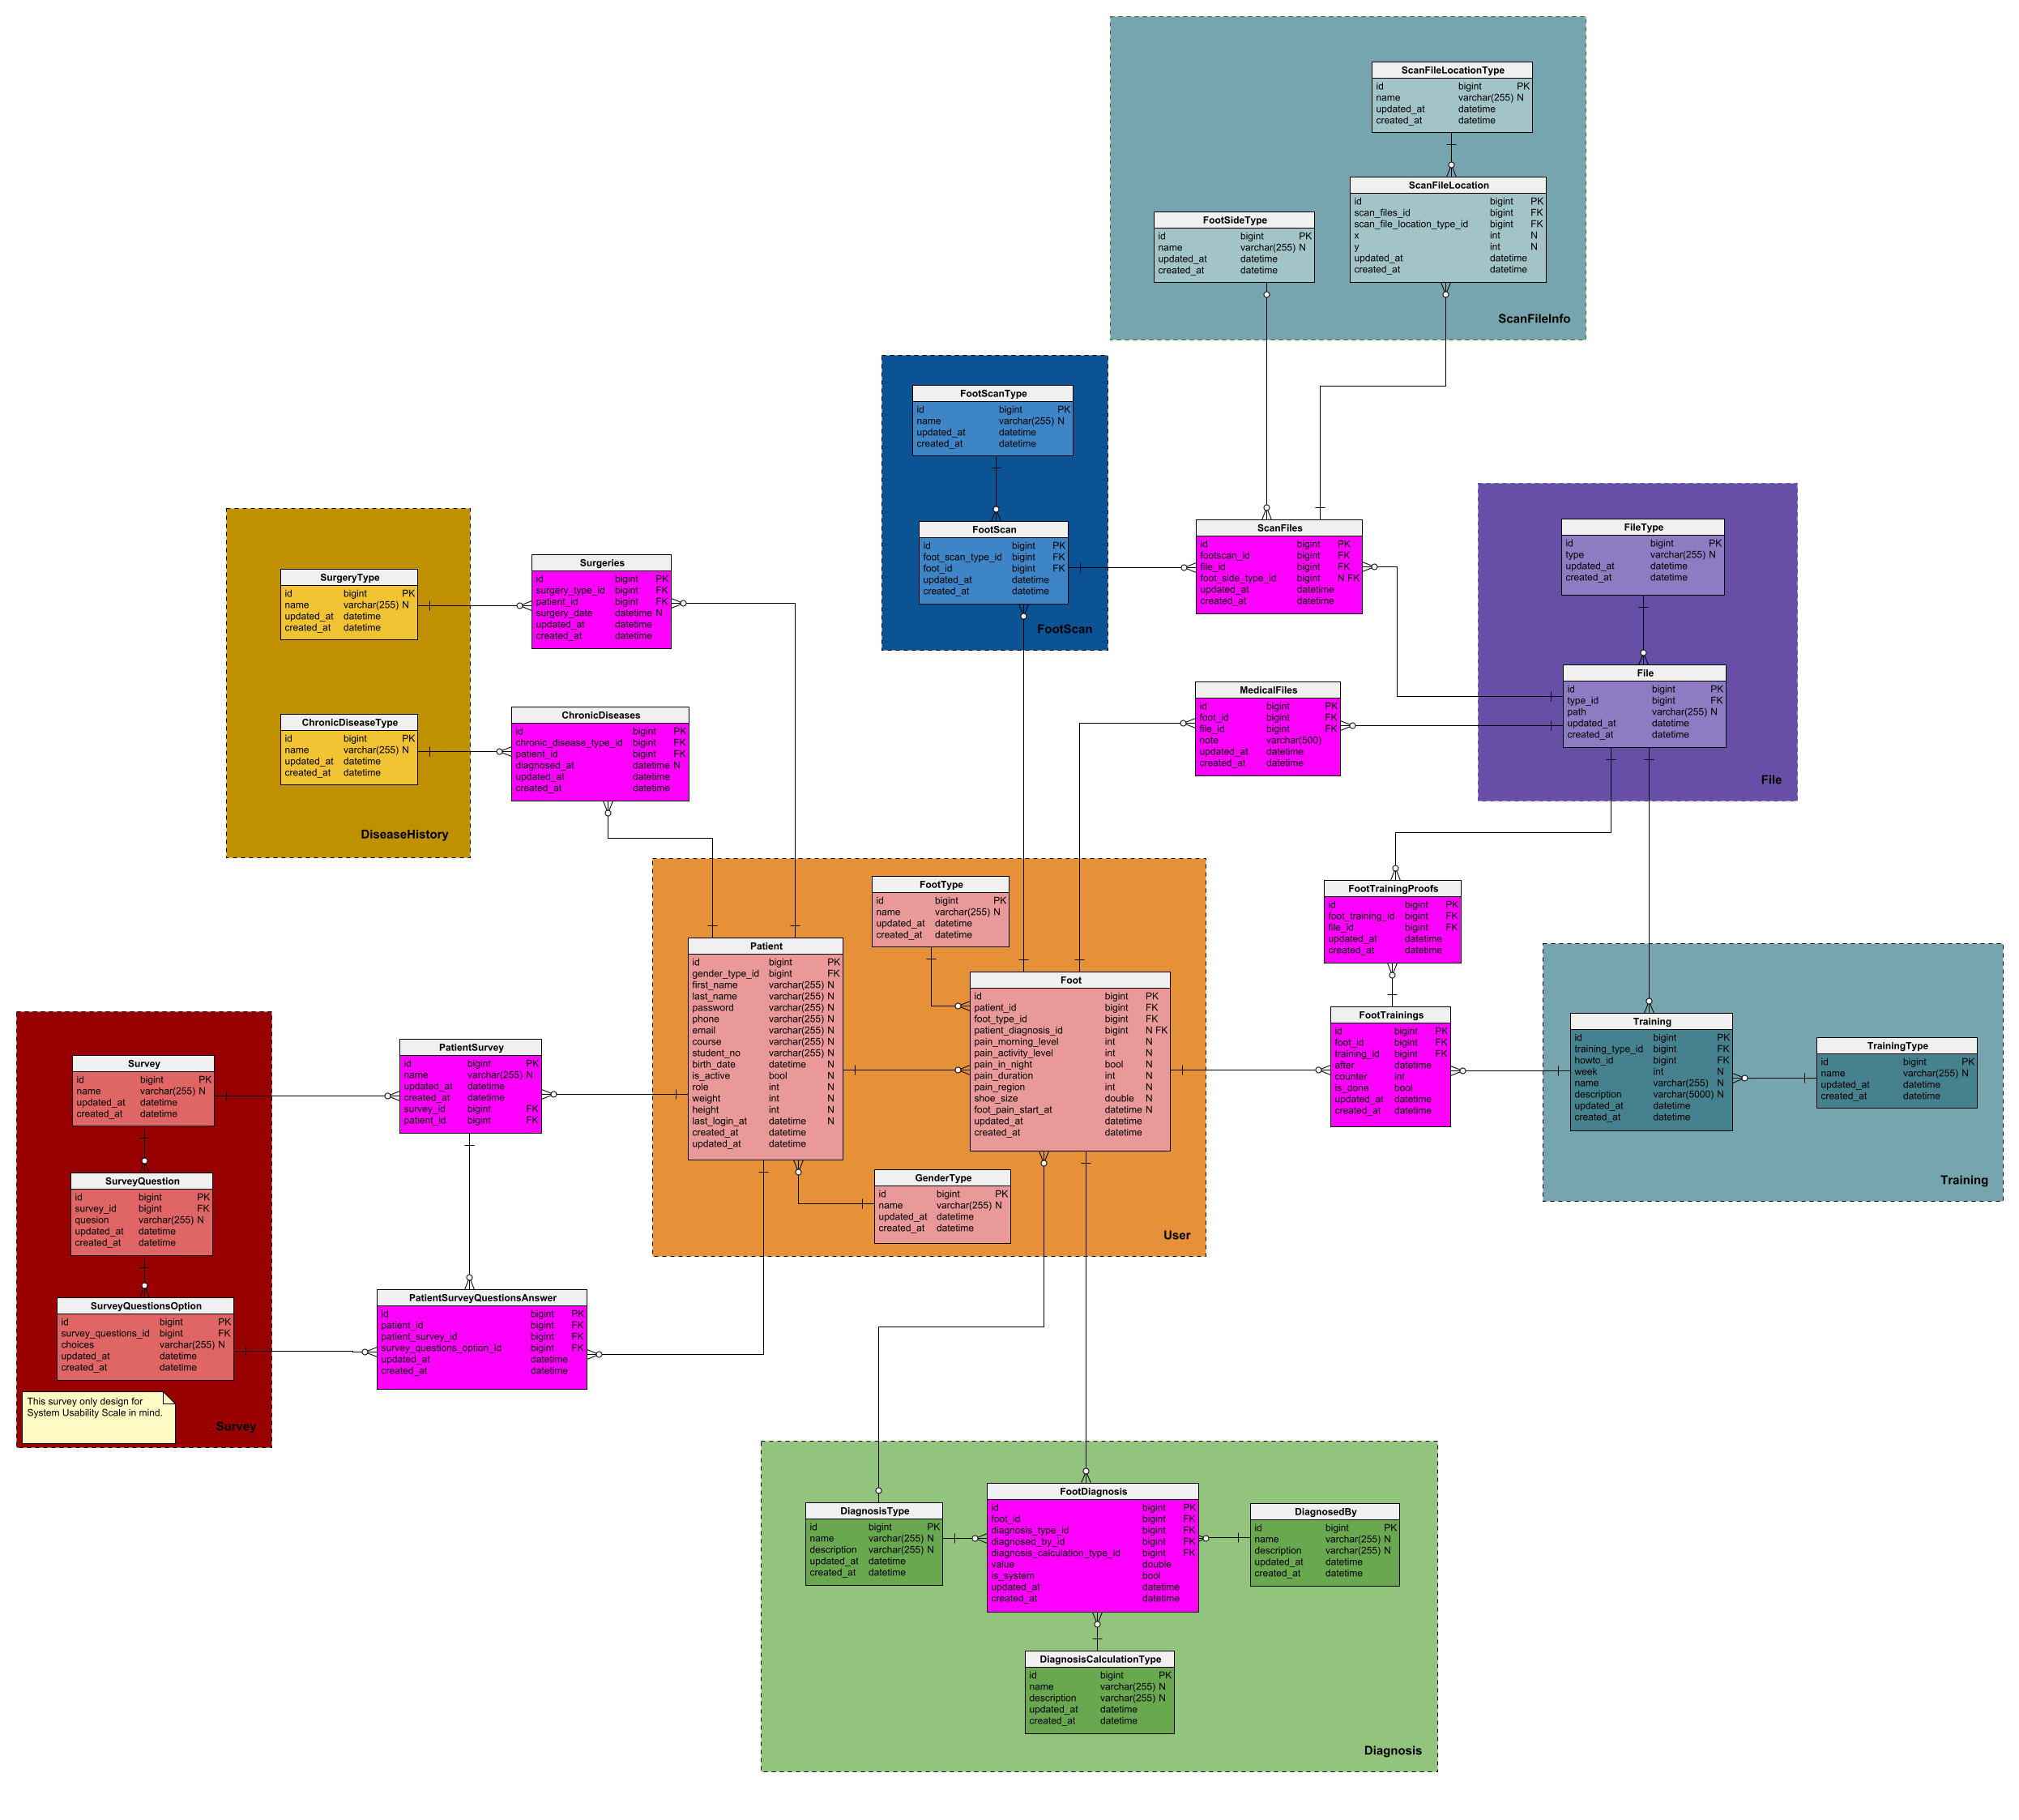
\includegraphics[width=1.0\columnwidth]{KaanEksenMSc/figures/DatabaseGeneralView.png}}
\caption{General view of database}
\label{fig:DatabaseGeneralView}
\end{figure}

User table group were explicitly designed for all application users, which includes end-users, healthcare professionals and admins. Its components consist of patient, foot, foot type, and gender (see Figure \ref{fig:DatabaseUser}). In addition, users have had roles that help generalize the table, such as healthcare specialists or patients. Furthermore, foot type was added for patients with different conditions, such as a prosthetic foot.

\begin{figure}[htbp]
\centering
\fbox{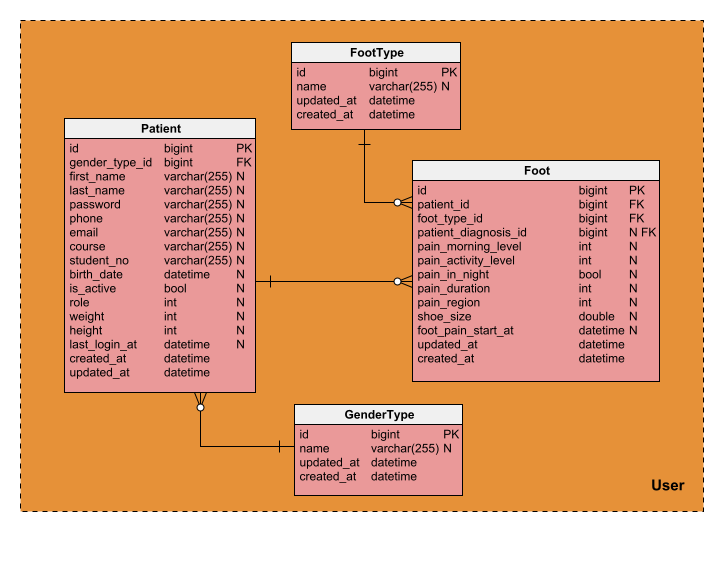
\includegraphics[width=.7\columnwidth]{KaanEksenMSc/figures/DatabaseUser.png}}
\caption{Database user group table}
\label{fig:DatabaseUser}
\end{figure}

The diagnosis table group focuses on foot diagnosis and detailed calculations methods (see Figure \ref{fig:DatabaseDiagnosis}). The foot may have multiple diagnoses from multiple healthcare specialists or the system. In addition, diagnoses calculation details can be recorded, such as the Staheli arch index.

\begin{figure}[htbp]
\centering
\fbox{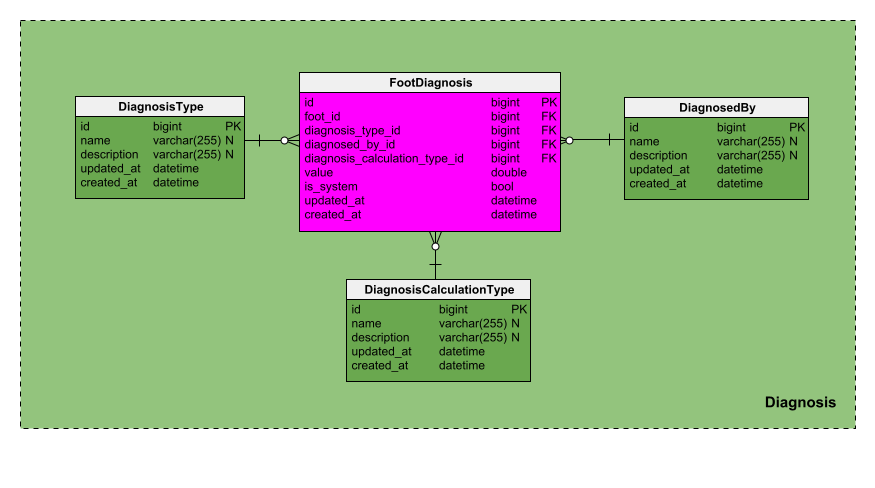
\includegraphics[width=.9\columnwidth]{KaanEksenMSc/figures/DatabaseDiagnosis.png}}
\caption{Database diagnosis group table}
\label{fig:DatabaseDiagnosis}
\end{figure}

The ScanFileInfo, FootScan, File table groups were designed to record patient assets according to the examination type (see Figure \ref{fig:DatabaseFiles}). FootScan records examination type such as Foot Deformity or Rom Measurement. Each examination can have unlimited images recorded in the ScanFiles table with a type such as Bottom, Back Side. Each image might have essential locations recorded in the ScanFileLocation table, such as the side thumb. In addition, file information such as file system locations is recorded in the File table, and each file contains a file type for processing.

\begin{figure}[htbp]
\centering
\fbox{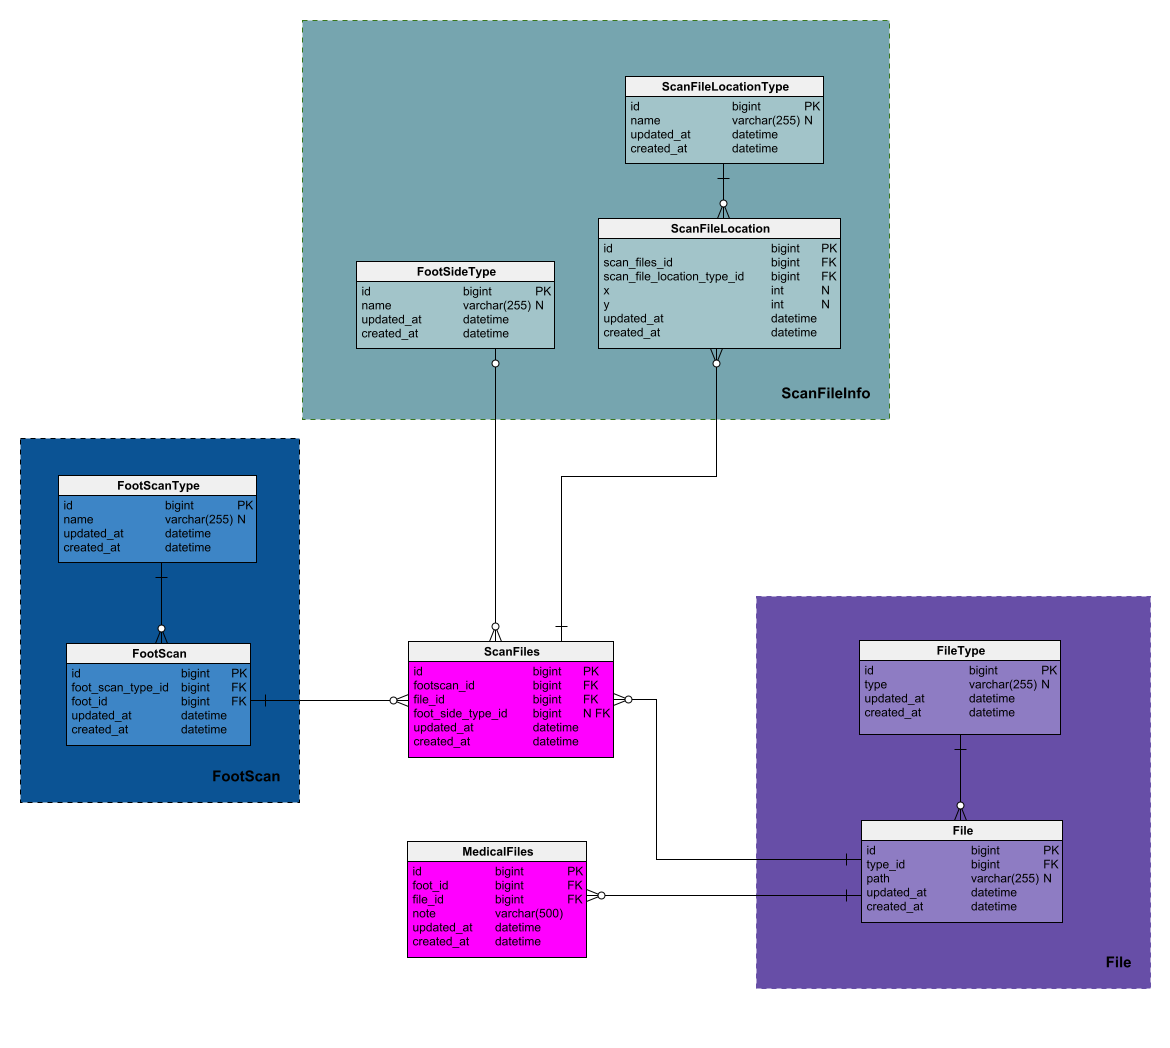
\includegraphics[width=.7\columnwidth]{KaanEksenMSc/figures/DatabaseFiles.png}}
\caption{Database files group}
\label{fig:DatabaseFiles}
\end{figure}

Survey and Training table groups are used for the feedback and healing after deformities are detected. Those tables help the healthcare professionals track the patients' activities. In addition, the DiseaseHistory table group is used to record the previous diseases and surgeries of the patients.

\section{TEST AND EVALUATION} \label{sec:StudyITestAndEvaluation}

In this section, the test and evaluation process of the prototype system, which was explained in detail in the previous sections, will be discussed.

In the first study, the test data were collected through mobile applications without any supervision. Therefore some of the data collected were not usable in the test and evaluation process. In addition, the data was mainly collected on the Yeditepe university students, which is a diverse population, and participants were provided with the how-to-use document.

\begin{table}[htbp]
\begin{center}
\caption{Participant statistics in study I}
\vspace{23pt}
      \begin{tabular}{|c|c|c|c|c|} \hline
          & \textbf{Age} & \textbf{Weight} & \textbf{Height} & \textbf{BMI} \\ \hline
        \textbf{Avarage} & 24.06 & 75.15 & 173.18 & 24.91 \\ \hline
        \textbf{Max} & 48 & 120 & 186 & 37.04 \\ \hline
        \textbf{Min} & 21 & 50 & 160 & 18.14 \\ \hline
    \end{tabular}
\label{tab:StudyIParticipantStatistics}
\end{center}
\end{table}

The prototype was used by 34 participants, where 12 (35.29 percent) of them were female, and the remaining 22 (64,71 percent) were male, with an average age of 24 (see Table \ref{tab:StudyIParticipantStatistics} for details). Data that were provided by participants were stored in an online database which is described in section \ref{sec:StudyIAnalysisAndDesign}. 

\begin{figure}[htbp]
\centering
\fbox{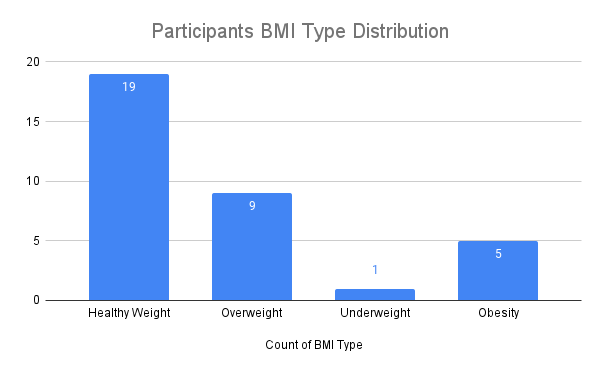
\includegraphics[width=.65\columnwidth]{KaanEksenMSc/figures/StudyIParticipantsBMITypeDistribution.png}}
\caption{Participants BMI type distribution based on CDC in study I}
\label{fig:StudyIParticipantsBMITypeDistribution}
\end{figure}

The average BMI in the population was calculated as 24.9. As seen in Figure \ref{fig:StudyIParticipantsBMITypeDistribution}, at least one person from each BMI category participated in the study. Therefore, this will provide sufficient data for projection.

The data collected from the users included 68 photos, 61 of them were used, but 7 of them were unusable because they were taken incorrectly. In addition, data collection was done in an unsupervised manner which caused seven unusable photos. All the data provided by the participants were shared with a physician through the specialist interface, which is described in sub-section \ref{sec:SpecialistInterface}. The physician went through all the system data and recorded critical points to the system.

\begin{figure}[htbp]
\centering
\fbox{\includegraphics[width=.65\columnwidth]{KaanEksenMSc/figures/StudyICriticalPointResult.png}}
\caption{Critical point results on study I}
\label{fig:StudyICriticalPointResult}
\end{figure}

After the physician results were collected, index calculations were conducted (see Figure \ref{fig:StudyICriticalPointResult}). Even with specialists' critical points, the results vary based on the index type. However, even if the reference points vary, approaching specialists' results will reveal the system's usability. Therefore, the initial study has been investigating the system set critical points, and the specialist set critical point differences.

\begin{figure}[htbp]
\centering
\fbox{\includegraphics[width=.65\columnwidth]{KaanEksenMSc/figures/StudyIIndexErrorNormalDists.png}}
\caption{Index error normal distribution in study I}
\label{fig:StudyIIndexErrorNormalDists}
\end{figure}

Initial results showed that the findings of the specialist and the system were 91.80 percent matched. Even though these results showed great promise, this comparison was based on the class of the foot. Therefore, a more quantitative approach was necessary to asset the conducted test was accurate. Since automated algorithm critical points are not directly comparable with the specialist critical points (the pre-diagnosis algorithm transforms the images), point intermediate and resulting findings were compared.

Therefore, the system index errors were calculated, and normal distribution was piloted (see Figure \ref{fig:StudyIIndexErrorNormalDists}). The results showed that most of the normal distribution of the index error was within a small error range. On the other hand, it has been observed that there are also outliers with significant error rates. These errors were primarily due to human errors, such as misplaced critical points or photos taken from the wrong angle. 

\begin{figure}[htbp]
\centering
\fbox{\includegraphics[width=.65\columnwidth]{KaanEksenMSc/figures/StudyILenghtErrorNormalDists.png}}
\caption{Length error normal distribution in study I}
\label{fig:StudyILenghtErrorNormalDists}
\end{figure}

In addition, length error was also calculated to see the effect of the perspective transformation in error calculation (see Figure \ref{fig:StudyILenghtErrorNormalDists}). Even though those results showed similar results to index error, outliers were increased. This error increase was partially due to a perspective transformation of the images.

\chapter{STUDY II - BACK SIDE DIAGNOSIS}\label{chp:Back Side Diagnosis}

In this chapter, an overview of the new pre-diagnosis (i.e., diagnosis based on back side of the foot) will be discussed—this system is based on achilles tendon. Accordingly, general system analysis and design decisions will be addressed in Section \ref{sec:StudyIIAnalysisAndDesign}. Then, specifics of implementation will be reviewed in Section \ref{sec:StudyIIImplementation}, and finally, the initial test results and evaluation phase will be discussed in Section \ref{sec:StudyIITestAndEvaluation}

\section{ANALYSIS AND DESIGN} \label{sec:StudyIIAnalysisAndDesign}

In this section, the basic structures of the system discussed in Chapter \ref{chp:Foot Detection & Primary Diagnosis} have not been changed while analyzing and designing. In addition, this chapter was profoundly focused on the small changes made to the system. Changes in requirements and design decisions will be discussed in this section.

As discussed in Section \ref{sec:StudyITestAndEvaluation}, a lack of supervision causes data to be unusable and unstable test environments. Therefore, the system should be used by healthcare officials or supervised while used by participants.

\begin{figure}[htbp]
\centering
\fbox{\includegraphics[width=.6\columnwidth]{KaanEksenMSc/figures/SystemOverviewStudyII.png}}
\caption{Architecture diagram of the updated system}
\label{fig:GeneralArchitectureDiagramPartI}
\end{figure}

Index results of healthcare professionals may conflict with each other due to remote image evaluations, which are discussed in Section \ref{sec:StudyITestAndEvaluation}. Therefore, healthcare professionals’ diagnosis results should be added after examinations to assess the diagnosis correctly. The general structure of the converted system can be seen in Figure \ref{fig:GeneralArchitectureDiagramPartI}.

\subsection{ Prediction And Fine Tune Module }

The prediction module consists of end-user interactions and pre-diagnosis. However, for improving results and getting more accurate test results, pre-diagnosis should be disabled since healthcare professionals will guide the participants. 

Another module, the fine-tune module, consists of background procedures and healthcare professionals' interactions. Also, the healthcare interaction module will not be used in this module since all deformities should be diagnosed on examination. In the following paragraphs, details of the changes will be discussed.

End-user interactions on the prediction module should be updated to be usable by the healthcare professionals for supervised data collection. The same application flow should be protected except for minor modifications. For example, healthcare professionals should be able to enter the diagnosis results of the patients into the application.

In the needs analysis, the importance of the Achilles tendon in the diagnosis process was discussed with the health professionals, and therefore it was decided to base the Achilles tendon in the automated index calculation process.

\subsection{ Index Calculation }

The pre-diagnosis, the system's underlying structure, which reduces the workload of healthcare professionals, should be updated to improve the results. Based on the importance of the Achilles tendon, the rearfoot angle is the best index calculation method for this calculation. 

Therefore, photographs of the back of the foot should be taken, and the rearfoot angle calculations should be made. These photos must include the calf and up to the foot's heel. In addition, legs should be centered for more accurate calculations.

\section{IMPLEMENTATION}\label{sec:StudyIIImplementation}

Implementation details of the changed modules will be discussed in this section. A more detailed explanation is provided by dividing it into subsections. 

\subsection{End-User Application}

In this section, there was no significant change in the end-user application, only minor changes have been made to improve usability. Since users are not directly using the application, some user identification options are removed, such as phone numbers. In addition, some of the optional fields for students are also removed, such as student numbers (see Figure \ref{fig:UserApplicationStudyIChanges}).

\begin{figure}[htbp]
\centering
\fbox{\includegraphics[width=.41\columnwidth]{KaanEksenMSc/figures/UserApplicationStudyIChanges.jpeg}}
\caption{Minor changes in end-user application in study I}
\label{fig:UserApplicationStudyIChanges}
\end{figure}

In addition to compliance with requirements analysis, some minor bugs such as default values and crashes have been fixed, and diagnostic results have been collected as if healthcare professionals had entered them, not as if they were taken from the patient.

\subsection{Services And Batch Process}

Except for minor adjustments and bug fixes, no significant changes in services have been made. Most of the changes were conducted in the batch process for different index calculations in the automated process. Therefore in this subsection, all the changes will be discussed. 

One of the most significant service adjustments is made in the API. Diagnosis by option is added, which were recorded in different fields in the database (see Section \ref{sec:StudyIDatabase} for details). In addition, user type control is added to prevent misconfiguration.

\begin{figure}[htbp]
\centering
\fbox{\includegraphics[width=.55\columnwidth]{KaanEksenMSc/figures/BatchProcessRioStudyII.jpeg}}
\caption{Region of interest results in study II}
\label{fig:BatchProcessRioStudyII}
\end{figure}

The batch process calculation is redesigned from the start. Initially, the image types are differentiated for processing the correct images with correct index types. Therefore, the foot side type (see Section \ref{sec:StudyIDatabase} for details) is used for differentiation in the scan file (i.e., image).

After the correct image selection, detecting the foot and leg is crucial. Therefore, deep learning algorithms are applied to extract the region of interest. Finally, DeepLabV3 is used based on the experiences obtained in Section \ref{sec:StudyIServicesAndBatchProcess} to detect the region of interest (see Figure \ref{fig:BatchProcessRioStudyII}).

Fallowing the region of interest detection, critical points are detected. There are four critical points in rearfoot angle calculation (see Section for details \ref{sec:MethodologyFootDeformityDetection}). Each point requires specific points to be detected in the leg. In addition, each point is very close to the midpoint of the leg (see Figure \ref{fig:BatchProcessDotsStudyII}).

\begin{figure}[htbp]
\centering
\fbox{\includegraphics[width=.55\columnwidth]{KaanEksenMSc/figures/BatchProcessDotsStudyII.png}}
\caption{Calculated critical points for rearfoot angle (red dots)}
\label{fig:BatchProcessDotsStudyII}
\end{figure}

The first point base of the calcaneus is calculated based on the region of interest. Processing starts from the bottom of the image, where the initial region is detected wideness of the area is recorded. In case of the region of interest errors, the processing is continued until 30 percent of the image width from the initial region detection. If new wideness is more significant than 50 percent of the initial detection, new area wideness is considered the calcaneus's base.

The second point determination is based on the assumption that the ankle is the thinnest area in the leg. Therefore, the narrowing of the leg is sought, following the first point discovery. After this region is found, it is considered the second broken point, which is 5 percent down by the region of interest. In addition, the third point has a similar discovery process. The only difference is that the third point is 5 percent up by the region of interest

The fourth point corresponds to the narrowing point of the calf. Therefore, after the third point is found, narrowing is sought in the region.

\section{TEST AND EVALUATION}\label{sec:StudyIITestAndEvaluation}

This section will provide the test end evaluation process of the prototype system described in detail in previous sections. 

\begin{table}[htbp]
\begin{center}
\caption{Participant statistics in study II}
\vspace{23pt}
      \begin{tabular}{|c|c|c|c|c|} \hline
          & \textbf{Age} & \textbf{Weight} & \textbf{Height} & \textbf{BMI} \\ \hline
        \textbf{Avarage} & 22.67 & 70.89 & 173.11 & 23.24 \\ \hline
        \textbf{Max} & 29 & 100 & 190 & 30.19 \\ \hline
        \textbf{Min} & 21 & 50 & 159 & 19.05 \\ \hline
    \end{tabular}
\label{tab:StudyIIParticipantStatistics}
\end{center}
\end{table}

In the second study, the test data were collected through mobile applications though healthcare officials supervision. Therefore collected data were evaluated before the process. In addition, healthcare officials were provided with the how-to-use document, which explains how to use the application. 

The prototype was used by 9 participants, where 3 (33.33 percent) of them were female, and the remaining 6 (66,67 percent) were male, with an average age of 22.6 (see Table \ref{tab:StudyIIParticipantStatistics} for details). Data is stored in an online database which is described in section \ref{sec:StudyIAnalysisAndDesign}. 

\begin{figure}[htbp]
\centering
\fbox{\includegraphics[width=.65\columnwidth]{KaanEksenMSc/figures/StudyIIParticipantsBMITypeDistribution.png}}
\caption{Participants BMI type distribution based on CDC in study II}
\label{fig:StudyIIParticipantsBMITypeDistribution}
\end{figure}

BMI is critical since most of the index calculations are based on the ratio to remove the effects of the weight. Population's average BMI is 23.2 (healthy weight), ( see Figure \ref{fig:StudyIIParticipantsBMITypeDistribution}). Therefore, this might not provide sufficient data for projection in different wight scales.

\begin{figure}[htbp]
\centering
\fbox{\includegraphics[width=.60\columnwidth]{KaanEksenMSc/figures/StudyIIFootDeformityTypeDistribution.png}}
\caption{Foot deformity type distribution in study II}
\label{fig:StudyIIFootDeformityTypeDistribution}
\end{figure} 

There were 18 foot photos out of 18 foot pictures for processing since all data were supervised. The healthcare specialists approved all the data provided to the system. Therefore participants' deformities are validated in the examination (see Figure  \ref{fig:StudyIIFootDeformityTypeDistribution}).

\begin{figure}[htbp]
\centering
\fbox{\includegraphics[width=.60\columnwidth]{KaanEksenMSc/figures/StudyIIFootDeformityAutomatedDegreesAndDeformityResults.png}}
\caption{Rear foot angle vs foot deformity in automated process results}
\label{fig:StudyIIFootDeformityAutomatedDegreesAndDeformityResults}
\end{figure} 

After the data collection, automated index calculations were conducted. Initial results showed that the findings of the healthcare officials and the system were 27,7 percent matched. This low performance may be caused by multiple factors such as image angle, color disorientation, assumptions in point location determination. However, the primary factor is sensitivity to rear foot angle calculation error, in which was the angle between the two lines was limited to five degrees (see Figure \ref{fig:StudyIIFootDeformityAutomatedDegreesAndDeformityResults}). 

\chapter{STUDY III - INNER SIDE DIAGNOSIS IMPROVEMENT }\label{chp:Inner Side Diagnosis Improvement}

This chapter focuses on arch high index calculation improvements with the data provided in Chapter \ref{chp:Back Side Diagnosis}. Accordingly, Section \ref{sec:StudyIIIAnalysisAndDesign} will cover analysis and design decisions. Then, in Section \ref{sec:StudyIIIImplementation}, delves into the specifics of implementation. Finally, the initial test findings and evaluation phase will be discussed in Section \ref{sec:StudyIIITestAndEvaluation}.

\section{ANALYSIS AND DESIGN}\label{sec:StudyIIIAnalysisAndDesign}

Preliminary detection of potential pes planus and pes cavus patients will be provided based on the inner side photographs of the foot. This system will be based on the initial implementation of the arch height index calculation discussed in Chapter \ref{chp:Foot Detection & Primary Diagnosis}. However, this chapter profoundly focuses on improving the batch process on pre-diagnosis.

Tree major fallbacks of the initial design were discovered in the test end evaluation of the process. All the fallbacks and potential solutions will be discussed in the following paragraphs.  

The first fallback is the differences between the line of the sole and the symmetry of the sole function. These differences should be reduced, and the foot function's sole should be more accurate.

The second fallback is that the bottom of the images contains a lot of noise in edge detection. By eliminating these noises, the accuracy of the sole foot function should be increased. The greedy approach could be used to improve accuracy with a relatively less computational resource.

The third fallback is that there is no error detection mechanism to reduce the error. Therefore, the sole function should not only be used for point detection but also for detecting the slope of the foot. As a result, this feature extraction should be used for detecting anomalies so that the results can be corrected.

\section{IMPLEMENTATION}\label{sec:StudyIIIImplementation}

Implementation details of the changes in the batch process will be discussed in this section. Each change will be separately discussed for a detailed explanation.

\begin{figure}[htbp]
\centering
\fbox{\includegraphics[width=.60\columnwidth]{KaanEksenMSc/figures/StudyIIIPredefinedWindows.jpeg}}
\caption{Accuracy improvement with polynomial regression window in study III}
\label{fig:StudyIIIPredefinedWindows}
\end{figure}

The first fallback is the accuracy of the sole function. The sole function generation was designed to reduce the sudden slope changes to the function because there might be an error in edge detection. Increasing the predefined windows, where polynomial regression is applied, will improve the function's response to changes (see Figure \ref{fig:StudyIIIPredefinedWindows}).

\begin{figure}[htbp]
\centering
\fbox{\includegraphics[width=.80\columnwidth]{KaanEksenMSc/figures/StudyIIINoiseReduce.jpg}}
\caption{Greedy noise reduce improvement in study III}
\label{fig:StudyIIINoiseReduce}
\end{figure}

The second fallback is that the edge images contain noise. Since the bottom of the images is changing based on the floor decoration,  removing the remaining edges on the floor will significantly improve the sole function accuracy. Since the foot has not contained edges in the bottom, actively removing the remaining edge 80 percent of points in the bottom should boost the accuracy (see Figure \ref{fig:StudyIIINoiseReduce}).

\begin{figure}[htbp]
\centering
\fbox{\includegraphics[width=.80\columnwidth]{KaanEksenMSc/figures/StudyIIISlopeCalculation.jpg}}
\caption{Slope calculation for error detection mechanism  in study III}
\label{fig:StudyIIISlopeCalculation}
\end{figure}

The last fallback is the absence of an error detection mechanism. With improved sole function, this can be achieved by calculating the function's slope in certain positions. The fact that the slope is higher than a specific rate is an indicator of pes cavus. Likewise, the same assumption can be made for the lack of slope. This error can be detected by taking two points in the foot; as the heel's peak and the foot space in the center (see Figure \ref{fig:StudyIIISlopeCalculation}).

\section{TEST AND EVALUATION}\label{sec:StudyIIITestAndEvaluation}

This section will provide the test end evaluation process of the prototype system described in detail in previous sections. In addition, thee were no data collection part. The third study uses the same data discussed in Section \ref{sec:StudyIITestAndEvaluation}. Therefore, the data collection and data details will be skipped.

\begin{figure}[htbp]
\centering
\fbox{\includegraphics[width=.60\columnwidth]{KaanEksenMSc/figures/StudyIIIFootDeformityAutomatedProcessResults.png}}
\caption{Foot deformity distribution in automated process results in study III}
\label{fig:StudyIIIFootDeformityAutomatedProcessResults}
\end{figure} 

Initial results showed that the findings of the healthcare officials and the system were 83,3\% matched. There were one pes planus two pes cavus mismatch detection recorded. Improved inner side test results are promising. However, the population was not diverse. Therefore system should be tested on larger population to get more accurate results.

\begin{figure}[htbp]
\centering
\fbox{\includegraphics[width=.60\columnwidth]{KaanEksenMSc/figures/StudyIIISlopeResults.png}}
\caption{Foot deformity distribution in automated process results in study III}
\label{fig:StudyIIISlopeResults}
\end{figure} 


\chapter{CONCLUSIONS AND FUTURE WORK}\label{chp:ConclusionsAndFutureWork}

This research aims to develop a mobile pre-diagnostic platform that will assists healthcare professionals in remotely classifying and evaluating possible patients with foot deformities that is namely pes cavus and pes planus. For this purpose, three studies were conducted to accurately detect pes planus and pes cavus. The first of these studis, unlike other studies, was conducted remotely and unsupervised, so the data are not used together with other studies.

The first study focused on the general flow and requirements of the system, and the detection of foot deformation was tested by remotely receiving and processing data throughout the study. Foot deformity determination was made according to the arch height index. Study results have been verified with data provided remotely by the expert. Although the initial research results were positive and resulted in high accuracy, it cannot be said that a guaranteed conclusion was reached about the first study results since the physician made the control with the data provided by the users and did not detect the foot deformation through physical examination. This study showed that pes planus and pes cavus detection is possible using mobile applications. Therefore, second study was conducted to verify the first study’s results by performing deformity detection under the supervision of healthcare professionals.

The second study focused on the acquisition of examination data and results of rearfoot angle based foot deformity detection algorithm. In this study, mobile applications were used by healthcare professionals and not by end users, to obtain supervised data. Some infrastructure changes were made to enable healthcare professionals to use the system as end-user, and as a result, more accurate data was collected. The second study shows that using a rearfoot angle based foot deformity detection algorithm was not possible for mobile based detection because the pre-diagnosis algorithm was susceptible to degree changes in the critical points lines (5 degrees). Therefore, third study was conducted to verify and improve the  arch height index algorithm

The third study focused on improving foot deformity detection. Throughout this study, the data collected by the healthcare professionals in the second study and the detection method in the first study were used. In this study, the results are significantly improved compared to the second study, while reducing the shortcomings of the arch height index introduced in the first study. The third study showed that pre-diagnose pes planus and pes cavus through a mobile phone application using image processing and deep neural networks is possible.

When the results of 3 studies are examined, the first study gives the best result with a success rate of 91.80 percent, but since the first study data were not obtained in a supervised manner, it cannot be compared with other studies. The success rates of the second and third studies are 27.7 percent and 83.3 percent, respectively. Accordingly, the results of the second study reveal the importance of selecting the correct index method for pre-diagnosis.

Although test trials were conducted in various populations, tests were carried out with limited participants, especially in the second and third studies. Therefore, the results in larger populations may be different.

Many different adaptations, experiments and studies could be done in the future. These are, first, that better results can be achieved by collecting more data and moving manual feature extraction to deep learning exercises, and secondly, problems in data collection can be eliminated by placing various controls in end-user applications and finally, the development of detection algorithms based on other pes planus and pes cavus diagnostic methods accepted in the literature.





%\bibliography{Main}


\bibliographystyle{packagesDonotChange/vancouver}
\bibliography{chapters/bibtexFile}


\setcounter{equation}{0}

\appendix
%\addcontentsline{toc}{chapter}{\numberline{}Appendix}


%% this part is used to remove table and figure in the appendix from the list of tables and figure so don't delete it
\let\svaddcontentsline\addcontentsline
\renewcommand\addcontentsline[3]{%
  \ifthenelse{\equal{#1}{lof}}{}%
  {\ifthenelse{\equal{#1}{lot}}{}{\svaddcontentsline{#1}{#2}{#3}}}}
  
%%  you can make change after this line %%
  





%%\begin{figure}[htbp]
%%\centering
%%\fbox{\includegraphics[width=.8\columnwidth]{figures/DNAhelical.eps}}
%%\caption{Structure of DNA, single stand and double helix.}
%%\label{fig:DNAhelical2}
%%\end{figure}


\end{document}

